%Chinh dong 380 tu 50 --> 10 o file extreport
\documentclass[13pt,a4paper]{extreport}
\usepackage[utf8]{inputenc}
\usepackage[utf8]{vietnam} %Bien dich duoc tieng Viet
\usepackage{amsmath,amsfonts,amssymb} %Font toan
\usepackage{type1cm}
\usepackage{graphicx}
\usepackage{subfigure}
\usepackage{caption}
\usepackage{longtable}
\usepackage{comment}
\usepackage{multirow}
\usepackage[unicode]{hyperref} %Tu dong tao bookmark
\hypersetup{colorlinks = false}
\usepackage{indentfirst} %Thut vao dau dong o tat ca cac doan
\usepackage{listings} %Dinh dang code
\usepackage{color} %Mau sac
\usepackage[left=3cm,right=2cm,top=3cm,bottom=3cm]{geometry} %Canh lề trái - phải - trên - dưới cho tài liệu
\definecolor{dkgreen}{rgb}{0,0.6,0}
\definecolor{gray}{rgb}{0.5,0.5,0.5}
\definecolor{mauve}{rgb}{0.58,0,0.82}

\lstset{frame=tb,
	language=C,
	aboveskip=3mm,
	belowskip=3mm,
	showstringspaces=false,
	columns=flexible,
	basicstyle={\small\ttfamily},
	numbers=left,
	numberstyle=\tiny\color{gray},
	keywordstyle=\color{blue},
	commentstyle=\color{dkgreen},
	stringstyle=\color{mauve},
	%numberstyle=\tiny\color{black},
	%keywordstyle=\color{black},
	%commentstyle=\color{black},
	%stringstyle=\color{black},
	breaklines=true,
	captionpos=t,
	breakatwhitespace=true,
	tabsize=2
}

\newcommand{\nocontentsline}[3]{}
\newcommand{\tocless}[2]{\bgroup\let\addcontentsline=\nocontentsline#1{#2}\egroup} 
\renewcommand{\arraystretch}{1.3}
\begin{document}
\begin{titlepage}
	\centering
	\begin{small}
\bfseries{TRƯỜNG ĐẠI HỌC KỸ THUẬT -- CÔNG NGHỆ CẦN THƠ\\KHOA ĐIỆN TỬ -- VIỄN THÔNG\\ \vspace{1cm}}
   \end{small}
	
\includegraphics[width=.3\textwidth]{CTUT_logo}\par\vspace{1cm}
	{\Large\bfseries ĐỒ ÁN MÔN HỌC VI ĐIỀU KHIỂN\vspace{.5cm}\par}
	{\Large\bfseries ĐỀ TÀI\vspace{.5cm}\par}
	{\Large\bfseries ĐỌC GIÁ TRỊ NHIỆT ĐỘ ĐIỀU KHIỂN\\ BƠM NƯỚC CỨU HỎA\par}
	\vspace{2cm}
	
	\begin{tabular}{ll}
	{\Large\itshape Giảng viên hướng dẫn:} & {\Large\itshape Thầy Đường Khánh Sơn}\vspace{.3cm}\\
	{\Large\itshape Nhóm sinh viên thực hiện:} &{\Large\itshape Nhóm 7}\vspace{.2cm}\\
		{\Large\itshape \hspace{1.5cm}1. Nguyễn Văn Đình}& {\Large\itshape -- MSSV: 1350353}\vspace{.2cm}\\
	{\Large\itshape \hspace{1.5cm}2. Thi Minh Nhựt}& {\Large\itshape -- MSSV: 1350366}\vspace{.2cm}\\
	{\Large\itshape \hspace{1.5cm}3. Phạm Thanh Quý}& {\Large\itshape -- MSSV: 1350222}\vspace{.2cm}\\
		{\Large\itshape \hspace{1.5cm}4. Liên Thái Trường}& {\Large\itshape -- MSSV: 1350358}\vspace{.2cm}\\
		{\Large\itshape \hspace{1.5cm}5. Lư Anh Tuấn}& {\Large\itshape -- MSSV: 1350240}\vspace{.2cm}\\
	\end{tabular}
	
	\vfill
	
	
	\vfill
	
% Bottom of the page
	{\large \textit{Cần Thơ\\ \today}\par}
\end{titlepage}
\pagenumbering{roman}
\tableofcontents

\listoffigures

\listoftables

\newpage
\pagenumbering{arabic}
\chapter*{Mở đầu}
\addcontentsline{toc}{chapter}{Mở đầu}
\vspace{-1cm}Trước hết, em xin chân thành cảm ơn thầy đã tạo điều kiện cho chúng em có cơ hội thực hành trên board mạch thực tế, ứng dụng lý thuyết về vi điều khiển PIC 16F887 vào lập trình điều khiển một số thiết bị ngoài vi, khai thác các chức năng của vi điều khiển, từ đó làm cơ sở để giải quyết các bài toán trong thực tế cần đến ứng dụng của vi điều khiển.\\

Về thiết bị thực tập gồm có: Kit BOOK 1, Adapter, cáp USB, cáp kết nối,\ldots{} cùng một số ngoại vi thay thế khác mà em chuẩn bị được để thực tập thêm, nhằm nâng cao khả năng lập trình của mình.\\

Các chương trình trong bài báo cáo được viết cho vi điều khiển PIC 16F887 bằng ngôn ngữ lập trình CCS. Với một số chương trình em có tham khảo thêm trên các diễn đàn, từ đó học hỏi và đúc kết lại để hoàn thành bài tập trong phần báo cáo.\\

Địa chỉ của một số trang web viết về vi điều khiển PIC và ngôn ngữ lập trình CCS mà em tìm hiểu được:
\begin{itemize}
\item \verb|picvietnam.com|
\item \verb|codientu.org|
\item \verb|dientuchiase.com|
\item \verb|ytuongnhanh.vn|
\item \verb|chiaseprojects.blogspot.com|
\item Kênh \verb|Youtube| \footnote{https://www.youtube.com/watch?v=NcjcOiDxC5I\&list=PLhFjtzzUovr\_22rUHg566bYU5s8LDKk7f} của tác giả Nguyễn Thanh Dâng, về PIC16F877A và MikroC.
\item \verb|ccsinfo.com|
\end{itemize}

Bên cạnh phần cứng đó là các phần mềm hỗ trợ: ngôn ngữ lập trình CCS, chương trình nạp PICkit 2, ngôn ngữ lập trình Matlab, phần mềm mô phỏng Protues. Em sử dụng ngôn ngữ \LaTeX{} để hoàn thành bài báo cáo vì khi làm việc nhiều với code thì \LaTeX{} sẽ giúp định dạng code đẹp hơn, dễ nhìn hơn và tài liệu viết ra cũng mang tính cấu trúc hơn.\\ %\footnote{Để định dạng được \textsf{code} cần có gói lệnh \textsf{listings}}

Trong bài báo cáo, ở mỗi bài em xin tóm tắt lại một số kiến thức trong tài liệu thực tập vi điều khiển của thầy để làm cơ sở giải bài tập thực hành. Mỗi bài tập em có trình bày định hướng cách giải quyết các bài tập theo cách suy nghĩ của em nên không thể tránh khỏi sai sót, mong thầy cho nhận xét để em có thể hoàn thiện bài báo cáo hơn.\\

Cuối cùng, qua đợt thực tập vi điều khiển PIC 16F887 em hy vọng bài báo cáo của em có thể làm tài liệu chia sẽ cho người mới bắt đầu học lập trình vi điều khiển với PIC 16F887 cần những bài thực hành cơ bản, theo em khi giải quyết các bài tập trong nội dung thực tập giúp cho em hiểu biết thêm về cách lập trình cho PIC 16F887.\\

Địa chỉ toàn bộ mã nguồn của bài báo cáo:
\begin{center}
\verb|https://github.com/thinhut/vdk-pic16f887/tree/master/VDK2016|
\end{center}
\begin{flushright}
\textit{Sinh viên thực hiện,}\vspace{.5cm}\\
\textit{Thi Minh Nhựt}
\end{flushright}
\part*{NỘI DUNG BÁO CÁO THỰC TẬP}
\addcontentsline{toc}{chapter}{NỘI DUNG BÁO CÁO THỰC TẬP}
\section*{Sơ đồ chân của PIC 16F887}
\begin{figure}[!h]
\begin{center}
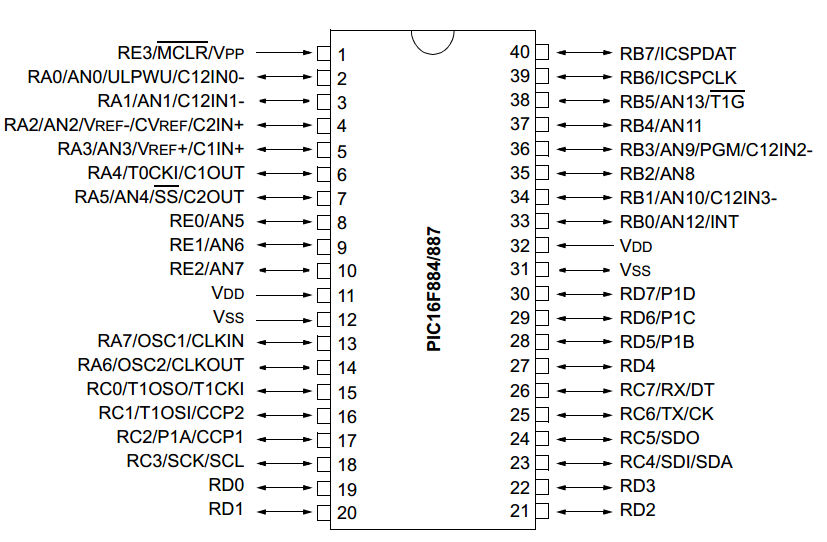
\includegraphics[scale=1]{image/PIC16F887}
\end{center}
\caption{Sơ đồ chân của PIC 16F887}
\end{figure}
\chapter{LED ĐƠN}
\label{Les:1}
\section{Giới thiệu chung}
\subsection{Yêu cầu}
Điều khiển các chân \verb|I/O| của PIC 16F887 với chức năng \verb|OUTPUT| thông qua chóp tắt các LED được nối với PORT E của vi điều khiển.
\subsection{LED}
LED là diode có khả năng phát ra ánh sáng hay tia hồng ngoại, tia tử ngoại. Có điện thế phân cực thuận từ $1.5 \div 3V$, điện thế phân cực ngược thấp.

Điện thế phân cực thuận của một số loại LED:
\begin{table}[!h]
\begin{center}
\begin{tabular}{|p{2.3cm}|c|}\hline
\centering{\textbf{Loại LED}} & \textbf{Điện thế phân cực thuận} \\ \hline
Đỏ & $1.4 \div 1.8V$\\ \hline
Vàng & $2.0 \div 2.5V$\\ \hline
Xanh lá cây & $2 \div 2.8V$\\ \hline
\end{tabular}
\end{center}
\caption{Điện thế phân cực thuận của một số LED}
\end{table}

Với các loại LED thường thì: $I_{max} = 30mA$. Còn LED loại siêu sáng thì điện áp phân cực thuận cao hơn LED thường (có loại lên đến $5V$), dòng $I_{max} = 30mA$.\\

Cách mắc điện trở hạn dòng cho LED:
\begin{list}{--}{}
\item Có $n$ LED mắc nối tiếp nhau:
\begin{align*}
R_{nt} = \frac{U_{\text{\textit{nguồn}}} - n \times U_{LED}}{I_{max}}
\end{align*}
\item Có $m$ nhánh đấu mắc song song (mỗi nhánh gồm $n$ LED nối tiếp):
\begin{align*}
R_{ss} = \frac{R_{nt}}{m}
\end{align*}
\item[$\ast$] Tùy theo yêu cầu về độ sáng của LED mà ta chọn giá trị của điện trở cho phù hợp.
\end{list}
\subsection{Sơ đồ mạch}
\begin{figure}[!h]
\begin{center}
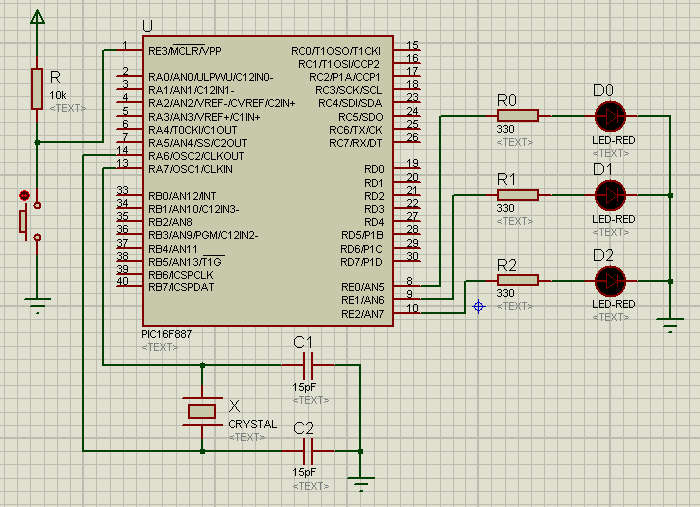
\includegraphics[scale=0.7]{bai-1/image/BAI-1}
\end{center}
\caption{Mạch điều kiển LED nối với PORT E}
\end{figure}
\section{Cách điều khiển các chân xuất nhập số}
PORT E có chức năng xuất nhập số \verb|I/O| và chức năng chuyển đổi \verb|ADC|. Ở đây chúng ta quan tâm đến chức năng xuất nhập số.
\paragraph{Cách điều khiển:}
\begin{itemize}
\item Xác định các chân của PORT E là chân \verb|OUTPUT| hay là \verb|INPUT|, dùng lệnh: \verb|TRISA| hoặc \verb|TRISB| hoặc \verb|TRISC| hoặc \verb|TRISD| hoặc \verb|TRISE|, ở đây mình điều khiển PORT E nên dùng \verb|TRISE|.
\begin{itemize}
\item Mỗi chân sẽ có một trạng thái là \verb|0| (chân \verb|OUTPUT|) hoặc \verb|1| (chân \verb|INPUT|).
\item Cả ba chân \verb|RE2, RE1, RE0| là chân \verb|OUTPUT| thì: \verb|TRISE = 0b000 = 0x00|, thứ tự bit là \verb|RE2-RE1-RE0| (tương tự như các PORT khác, theo thứ tự là chân có chỉ số cao đến chân có chỉ số thấp).

Ví dụ: \verb|RE2 - INPUT|, \verb|RE1,RE0 - OUTPUT| thì: \verb|TRISE = 0b100 = 0x04|, tương tự như các trường hợp khác của các PORT còn lại.
\item Để đơn giản cho việc lập trình, chúng ta có thể khai báo mã ở dạng nhị phân \verb|0b...| hoặc khai báo mã dạng thập lục phân \verb|0x...| (mã hex).
\end{itemize}
\item Nếu là chân \verb|OUTPUT| thì dùng \verb|0| (mức thấp) hoặc \verb|1| (mức cao) để thể hiện trạng thái của một chân.

Ví dụ: \verb|RE2,RE1,RE0| -- chân \verb|OUTPUT| ở mức cao thì: \verb|PORTE = 0b111 = 0x07|; \verb|RE2| -- chân \verb|OUTPUT| ở mức cao, \verb|RE1,RE0| -- chân \verb|OUTPUT| ở mức thấp thì: \verb|PORTE = 0b100| \verb|= 0x04| 
\item Nếu là chân \verb|INPUT|, thì phải đọc tín hiệu của chân đó (được xét ở bài sau).
\item Một số hàm hổ trợ: \verb|delay_ms(số mili giây)| hoặc \verb|delay_us(số micro giây)|, các cấu trúc lập trình \verb|for, while, if, if ... else,|\ldots
\end{itemize}
\section{Bài tập}
Trong chương trình có sử dụng thư viện \verb|DEF_887.H| (trong \emph{phụ lục \ref{def:887} trang \pageref{def:887}}).
\subsection{Bài tập 1.1}
\paragraph{Yêu cầu}Viết chương trình chóp tắt LED ở PORT E với thời gian delay $250ms$.
\paragraph{Hướng giải quyết} 
\begin{itemize}
\item Khai báo các chân ở PORT E là chân \verb|OUTPUT|: \verb|TRISE = 0x00|.
\item Lặp lại quá trình sau (dùng cấu trúc \verb|while|): LED tắt (\verb|PORTE = 0x00|); giữ trạng thái cũ $250ms$ (\verb|delay_ms(250)|); LED sáng (\verb|PORTE = 0b111 = 0x07|); giữ trạng thái cũ $250ms$ (\verb|delay_ms(250)|). Theo cách lập trình này ta có \textit{Chương trình 1}.
\item[$\ast$] \textit{Cách khác}: đầu tiên cho LED tắt (\verb|PORTE = 0x00|). Lặp lại quá trình: đảo trạng thái của LED (\verb|PORTE = | $\sim$\verb|PORTE|); giữ trạng thái cũ $250ms$ (\verb|delay_ms(250)|). Theo cách lập trình này ta có \textit{Chương trình 2}.
\end{itemize}
\newpage
\subsection*{Chương trình 1}
\lstinputlisting[language=C]{BAI-1-1.C}
\subsection*{Chương trình 2}
\lstinputlisting[language=C]{BAI-1-1v2.C}
\newpage
\subsection{Bài tập 1.2}
\paragraph{Yêu cầu}Viết chương trình chóp tắt LED ở PORT E với thời gian delay $1s$.
\paragraph{Hướng giải quyết} Ta sử dụng hàm \verb|delay_ms(số mili giây)| với tham số truyền vào là $1000$. Hàm \verb|delay_ms(số mili giây)| có tham số \verb|'số mili giây'| có giá trị $0 - 65535$ (\verb|int16|).
\paragraph{Chương trình}Sử dụng lại \textit{Chương trình 1} hoặc \textit{Chương trình 2}, thay đổi \verb|delay_ms(250)| thành \verb|delay_ms(1000)|.
\subsection{Bài tập 1.3}\label{Exe:1-3}
\paragraph{Yêu cầu}Viết chương trình chóp tắt LED ở chân \verb|RE1| với thời gian delay $1s$ và LED ở chân \verb|RE2| với thời gian delay là $0.5s$.
\paragraph{Hướng giải quyết}
\begin{itemize}
\item Với yêu cầu thì 2 LED thực hiện chóp hoặc tắt cùng một lúc khi mới vào chu kỳ đầu, nhưng phải đảm bảo đúng được chu kỳ của mỗi LED, với thời gian delay khác nhau, nên chia ra các trường hợp sau (để đảm bảo đúng thời gian \verb|delay|):
\begin{center}
\begin{tabular}{|c|c|c|c|}\hline
Thời gian & LED ở \verb|RE2| & LED ở \verb|RE1| & \verb|PORTE| \\ \hline
$0ms$ & \verb|ON| & \verb|ON| & \verb|0b110 = 0x06|\\ \hline
$500ms$ & \verb|OFF| & \verb|ON| & \verb|0b010 = 0x02|\\ \hline
$1000ms$ & \verb|ON| & \verb|OFF| & \verb|0b100 = 0x04| \\ \hline
$1500ms$ & \verb|OFF| & \verb|OFF| & \verb|0b000 = 0x00| \\ \hline
$2000ms$ & \multicolumn{3}{c|}{Lặp lại trạng thái}\\ \hline
\end{tabular}
\end{center}
\item Dựa vào bảng trên, ta viết được \emph{chương trình 3} thỏa yêu cầu.
\end{itemize}
\newpage
\subsection*{Chương trình 3}
\lstinputlisting[language=C]{BAI-1-3.C}


\chapter{HIỂN THỊ KÝ TỰ TRÊN LCD} \label{Les:LCD}
\section{Giới thiệu chung}
\subsection{Yêu cầu}
Viết chương trình hiển thị ký tự lên LCD.
\subsection{LCD}
Chức năng các chân của LCD:
\begin{table}[!h]
\begin{center}
\begin{longtable}{|c|c|p{5cm}|p{4.5cm}|l}\cline{1-4}
\textbf{STT} & \textbf{Ký hiệu} & \centering{\textbf{Mô tả}} & \centering{\textbf{Giá trị}} & \\ \cline{1-4}
1 & VSS & GND & $0V$ & \\ \cline{1-4}
2 & VCC & & $5V$ & \\ \cline{1-4}
3 & VEE & Tùy chỉnh độ tương phản & & \\ \cline{1-4}
\multirow{2}{.5cm}{ 4} & \multirow{2}{.8cm}{RS} & \multirow{2}{5cm}{Lựa chọn thanh ghi} & RS = 0: ghi lệnh & \\
& & & RS = 1: ghi dữ liệu & \\ \cline{1-4}
\multirow{2}{.5cm}{5} & \multirow{2}{.8cm}{R/W} & \multirow{2}{5cm}{Chọn thanh ghi đọc/viết dữ liệu} & R/W = 0: viết dữ liệu & \\
& & & R/W = 1: đọc dữ liệu & \\ \cline{1-4}
6 & E & Enable & & \\ \cline{1-4}
$7-10$ & DB0 -- BD3 & \multirow{2}{5cm}{Chân chuyền dữ liệu} & \multirow{2}{5cm}{8 bit từ $DB0 \rightarrow DB7$} & \\ 
$11-14$ & DB4 -- DB7 &  & & \\ \cline{1-4} 
%9 & DB2 &  & & \\  
%10 & DB3 &  & & \\  
%11 & DB4 &  & & \\  
%12 & DB5 &  & & \\  
%13 & DB6 &  & & \\  
%14 & DB7 &  & & \\ \cline{1-4}
15 & A & Cực dương của LED nền & $0 - 5V$& \\ \cline{1-4}
16 & K & Cực âm của LED nền & $0V$ & \\ \cline{1-4}
\end{longtable}
\end{center}
\caption{Sơ đồ chân và chứa năng các chân của LCD}
\label{Fig:lcd}
\end{table}
%\newpage

Ngoài sử dụng LCD, người ta còn sử dụng các LED 7 đoạn, LED ma trận để hiển thị dữ liệu (với LED 7 đoạn có trong \textit{phụ lục \ref{app:led-7-doan} trang \pageref{app:led-7-doan}}).
\subsection{Sơ đồ mạch}
\begin{figure}[!h]
\begin{center}
%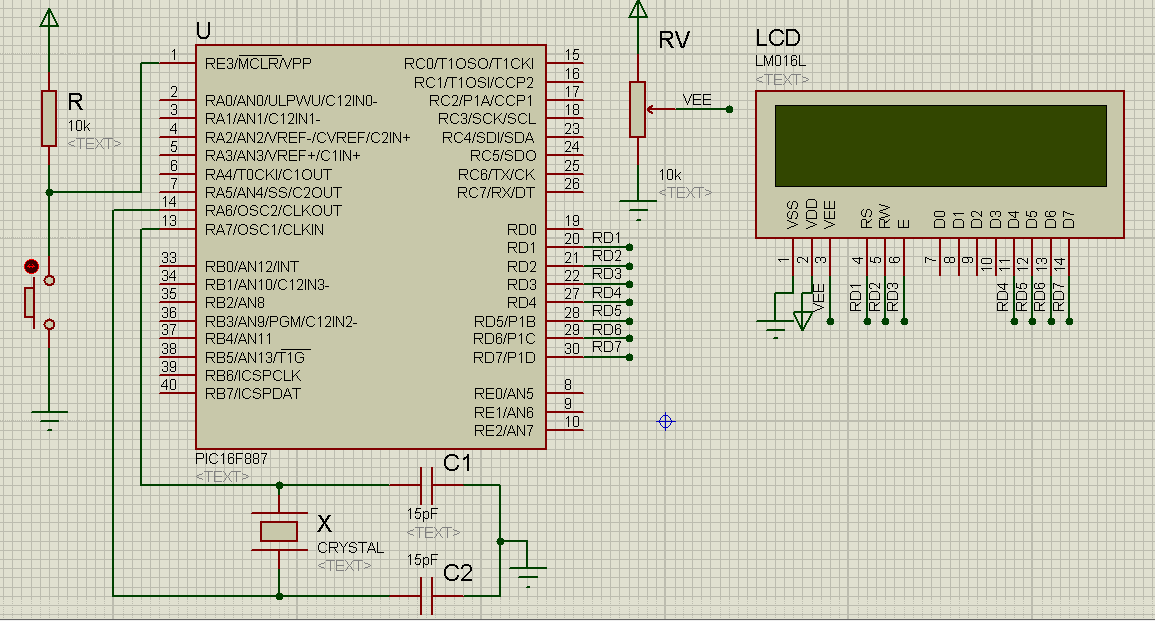
\includegraphics[width=3cm, height=4cm]{bai-2/image/BAI-2}
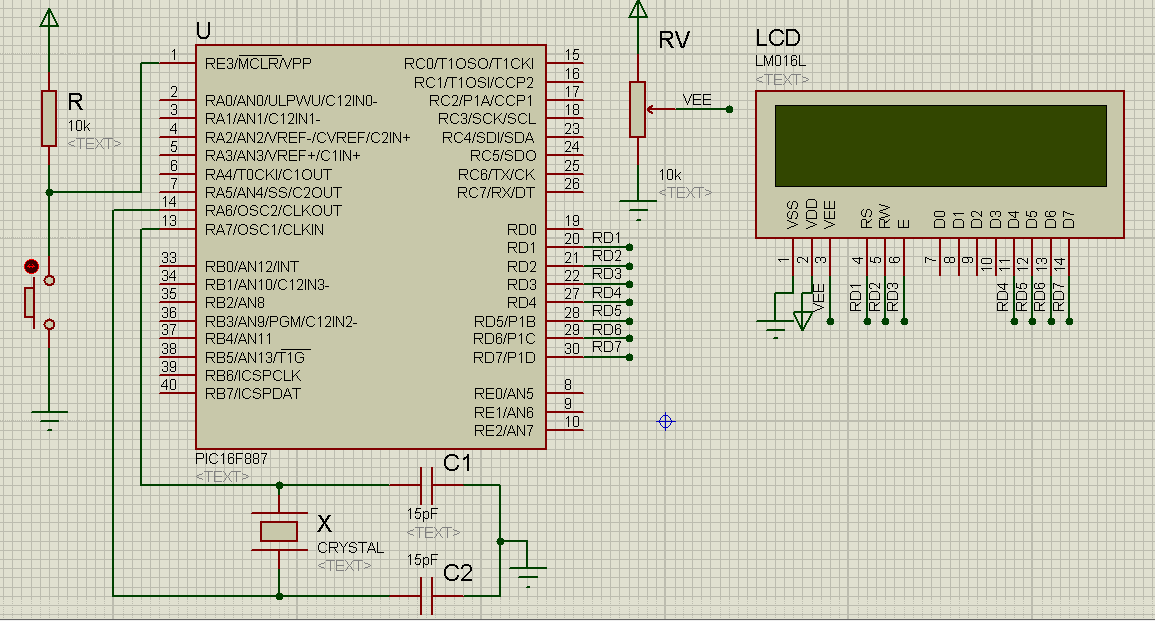
\includegraphics[scale=0.5]{bai-2/image/BAI-2}
\end{center}
\caption{Mạch điều khiển LCD}
\end{figure}
\section{Sử dụng các lệnh cơ bản cho LCD}
Sử dụng thư viện \verb|LCD_LIB_4BIT.C| (trong \emph{phụ lục trang \pageref{def:lcd}}) để điều khiển LCD.

Các bước cơ bản đề bắt đầu làm việc với LCD:
\begin{itemize}
\item Thêm thư viện LCD vào chương trình: \verb|#include<LCD_LIB_4BIT.C>|
\item Chúng ta dùng LCD ở chế độ ghi, dùng lệnh: \verb|OUTPUT_LOW(LCD_RW);| (trong \emph{bảng \ref{Fig:lcd} trang \pageref{Fig:lcd}}).
\item Khởi tạo LCD, dùng hàm: \verb|LCD_Init();|
\item Chức năng của một số hàm có trong thư viện được sử dụng:
\begin{itemize}
\item Hàm \verb|LCD_Init();| Khởi tạo LCD.
\item Hàm \verb|LCD_PutCmd(unsinged int cX);| Gửi lệnh lên LCD.

Ví dụ: \verb|LCD_PutCmd(0x01);| -- lệnh xóa màn hình.
\item Hàm \verb|LCD_PutChar(unsinged int cX);| Ghi một chuỗi hoặc một ký tự lên LCD.
\item Hàm \verb|LCD_SetPosition(unsinged int cX);| Thiết lập vị trí con trỏ.
\begin{itemize}
\item Dòng 1: bắt đầu từ vị trí \verb|0x00|, tăng giá trị này lên để đến các vị trí khác trên dòng 1.
\item Dòng 2: bắt đầu từ vị trí \verb|0x40|, tăng giá trị này lên để đến các vị trí khác trên dòng 2.
\end{itemize}
\end{itemize}
\item Cách sử dụng hàm \verb|printf(tham số)|: 
\begin{itemize}
\item Xuất chuỗi, ký tự: \verb|printf("Chuỗi, ký tự cần xuất");|
\item Xuất số nguyên: \verb|printf("N = %d",n);| số nguyên ngắn dùng \verb|%d|, số nguyên dài dùng \verb|%lu|
\item Xuất số thực: \verb|printf("A = %.2f",a);| quy định số chữ số sau dấy phẩy (trong ví dụ: quy định $2$ chữ số sau dấu phẩy).
\end{itemize}
\item Các cấu trúc: \verb|while, for, if, if...else,|\ldots
\end{itemize}
\section{Bài tập}
\subsection{Bài tập 2.1}
\paragraph{Yêu cầu}Viết chương trình hiển thị các ký tự sau lên LCD: \verb|DAI HOC KTCN CAN THO|
\paragraph{Hướng giải quyết}
\begin{itemize}
\item Thiết lập LCD ở chế độ ghi: \verb|OUTPUT_LOW(LCD_RW);|
\item Khởi tạo LCD: \verb|LCD_Init();|
\item Xóa màn hình: \verb|LCD_PutCmd(0x01);|
\item Ghi ký tự lên LCD:
\begin{itemize}
\item Cài đặt vị trí con trỏ: ta chọn vị trí thứ 6 -- \verb|LCD_SetPosition(0x05);| để ghi chuỗi \verb|"DAI HOC"| trên dòng 1.

Chọn vị trí thứ 3 -- \verb|LCD_SetPosition(0x42);| để ghi chuỗi \verb|"KTCN CAN THO"| trên dòng 2.
\item Ghi chuỗi: \verb|LCD_PutChar("DAI HOC");| và \verb|LCD_PutChar("KTCN CAN THO");|
\end{itemize}
\end{itemize}
\newpage
\section*{Kết quả}
\begin{figure}[!h]
%\vspace{-.5cm}
\begin{center}
  {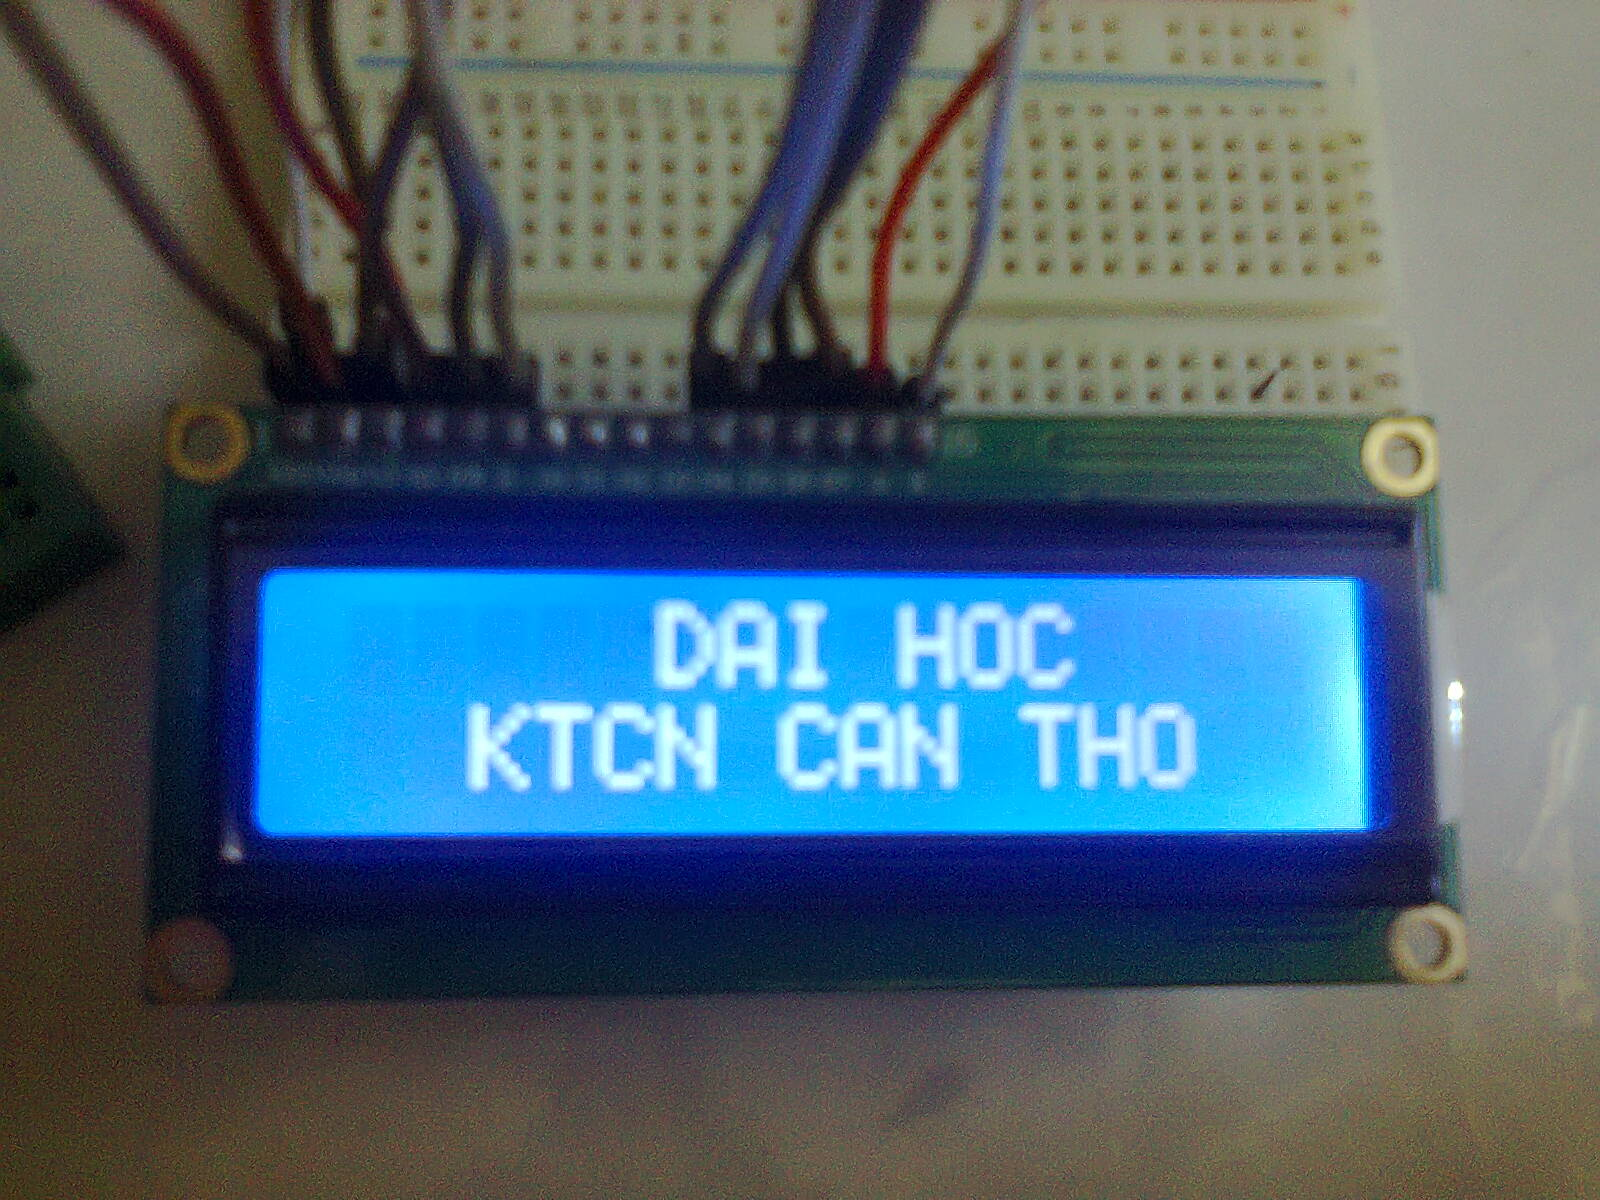
\includegraphics[width=.5\linewidth]{bai-2/image/2-1}}
\end{center}
\caption{Kết quả hiển thị ký tự lên LCD 16x02}
\end{figure}
\subsection*{Chương trình 4}
\lstinputlisting[language=C]{BAI-2-1.C}
\subsection{Bài tập 2.2}
\paragraph{Yêu cầu}Viết chương trình hiển thị trên \verb|LCD| theo yêu cầu sau: Hàng thứ nhất hiển thị họ tên sinh viên; hàng thứ hai hiển thị mã số sinh viên.
\paragraph{Hướng giải quyết}Sử dụng lại \emph{chương trình 4} của \emph{bải tập 2.1} với các thay đổi: vị trí con trỏ và chuỗi ký tự để phù hợp với yêu cầu.
\subsection*{Kết quả}
\begin{figure}[!h]
\begin{center}
  {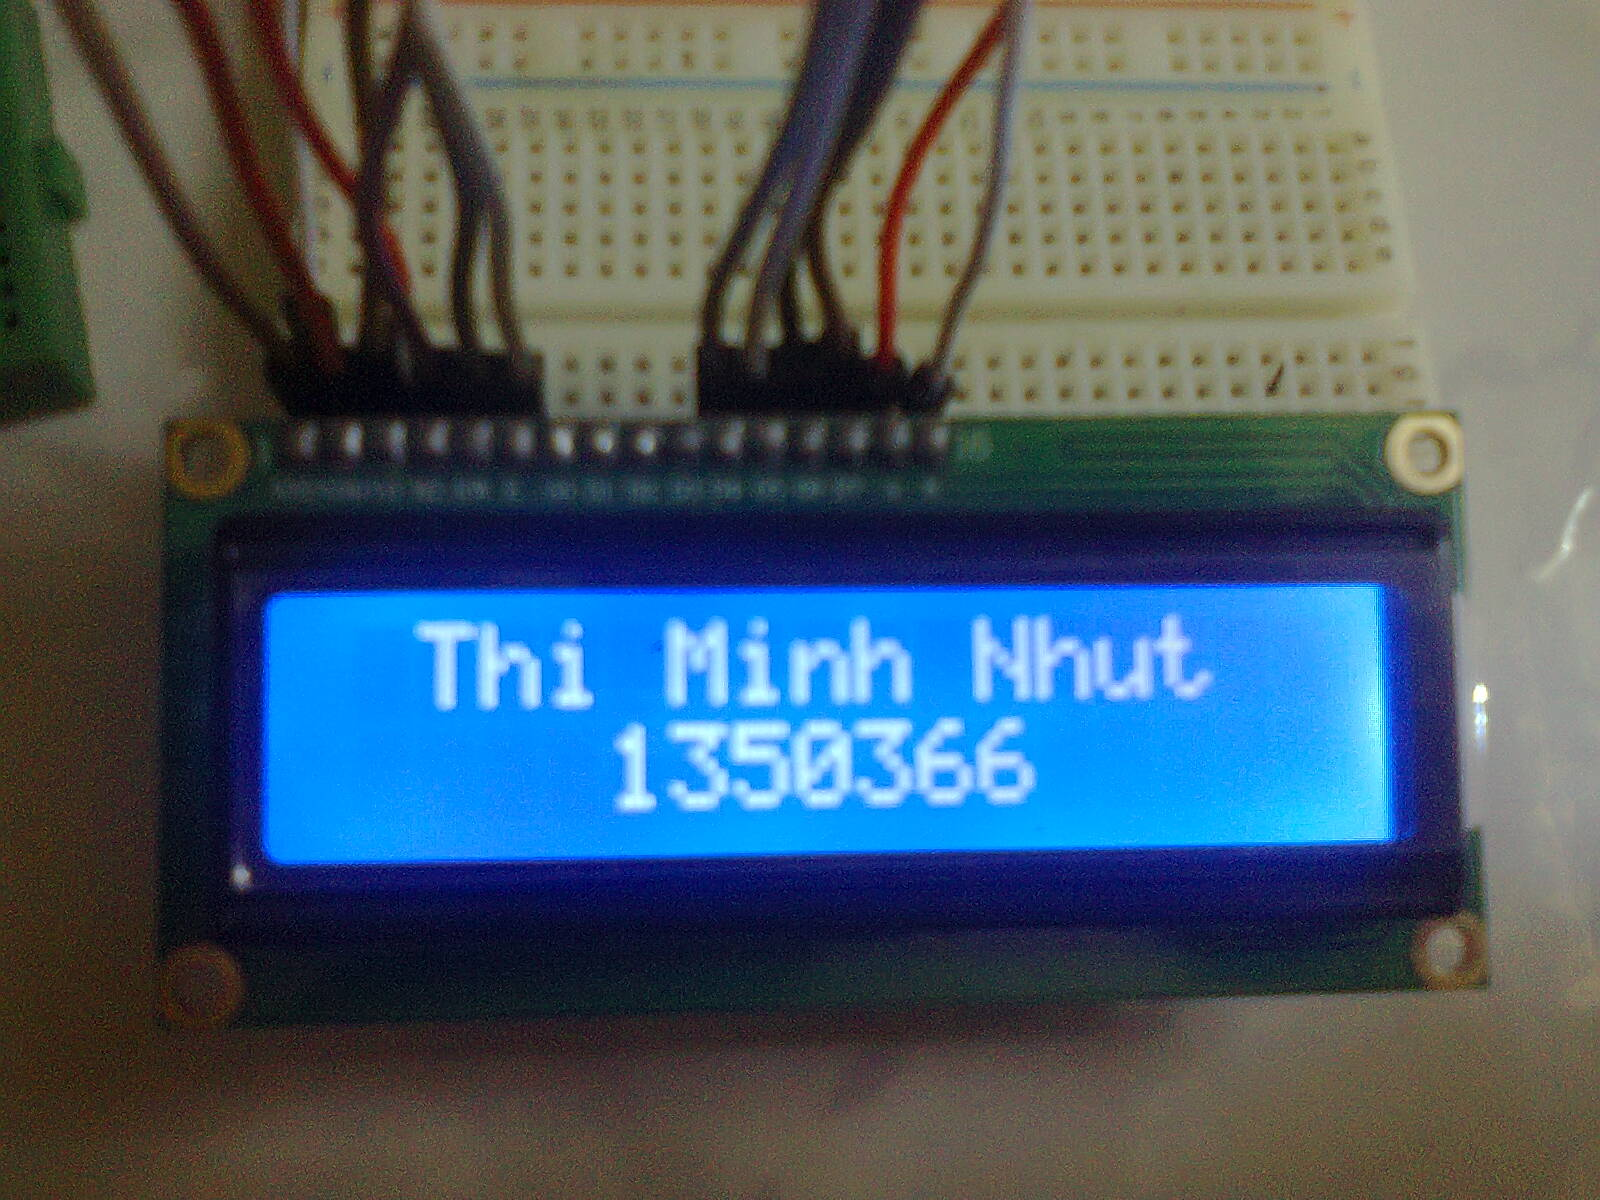
\includegraphics[width=.5\linewidth]{bai-2/image/2-2}}
\end{center}
\caption[]{Kết quả hiển thị họ tên và mã số sinh viên lên LCD 16x02}
\end{figure}
\subsection*{Chương trình 5}
\lstinputlisting[language=C]{BAI-2-2.C}
\subsection{Bài tập 2.3}
\paragraph{Yêu cầu}Viết chương trình đếm số từ $0$ đến $999$ hiển thị lên LCD.
\paragraph{Hướng giải quyết}
\begin{itemize}
\item Phần khai báo giống như \emph{bài tập 2.1}
\item Tăng giá trị số đếm: ban đầu ta gán biến đếm là \verb|count = 0;| rồi sử dụng cấu trúc \verb|for| để tăng giá trị biến đếm lên (\verb|count++;|)
\item Do cần hiển thị số lên LCD nên ta dùng hàm \verb|LCD_PutChar| kết hợp với hàm \verb|printf| để làm việc này.
\begin{itemize}
\item Hiển thị số nguyên: ví dụ \verb|unsigned long n = 12345| thì dùng:

\verb|printf(LCD_PutChar,"%lu",n);|
\item Hiển thị số thực: ví dụ \verb|float n = 1.2345 | thì dùng:

\verb|printf(LCD_PutChar,"%.4f",n);|
\end{itemize}
\item Để hiển thị giá trị biến đếm lên LCD, dùng:

\verb|printf(LCD_PutChar,"%lu",count);|

khi \verb|count| vượt quá giá trị, đưa biến \verb|count = 0;|
\end{itemize}
\subsection*{Kết quả}
\begin{figure}[!h]
\begin{center}
  {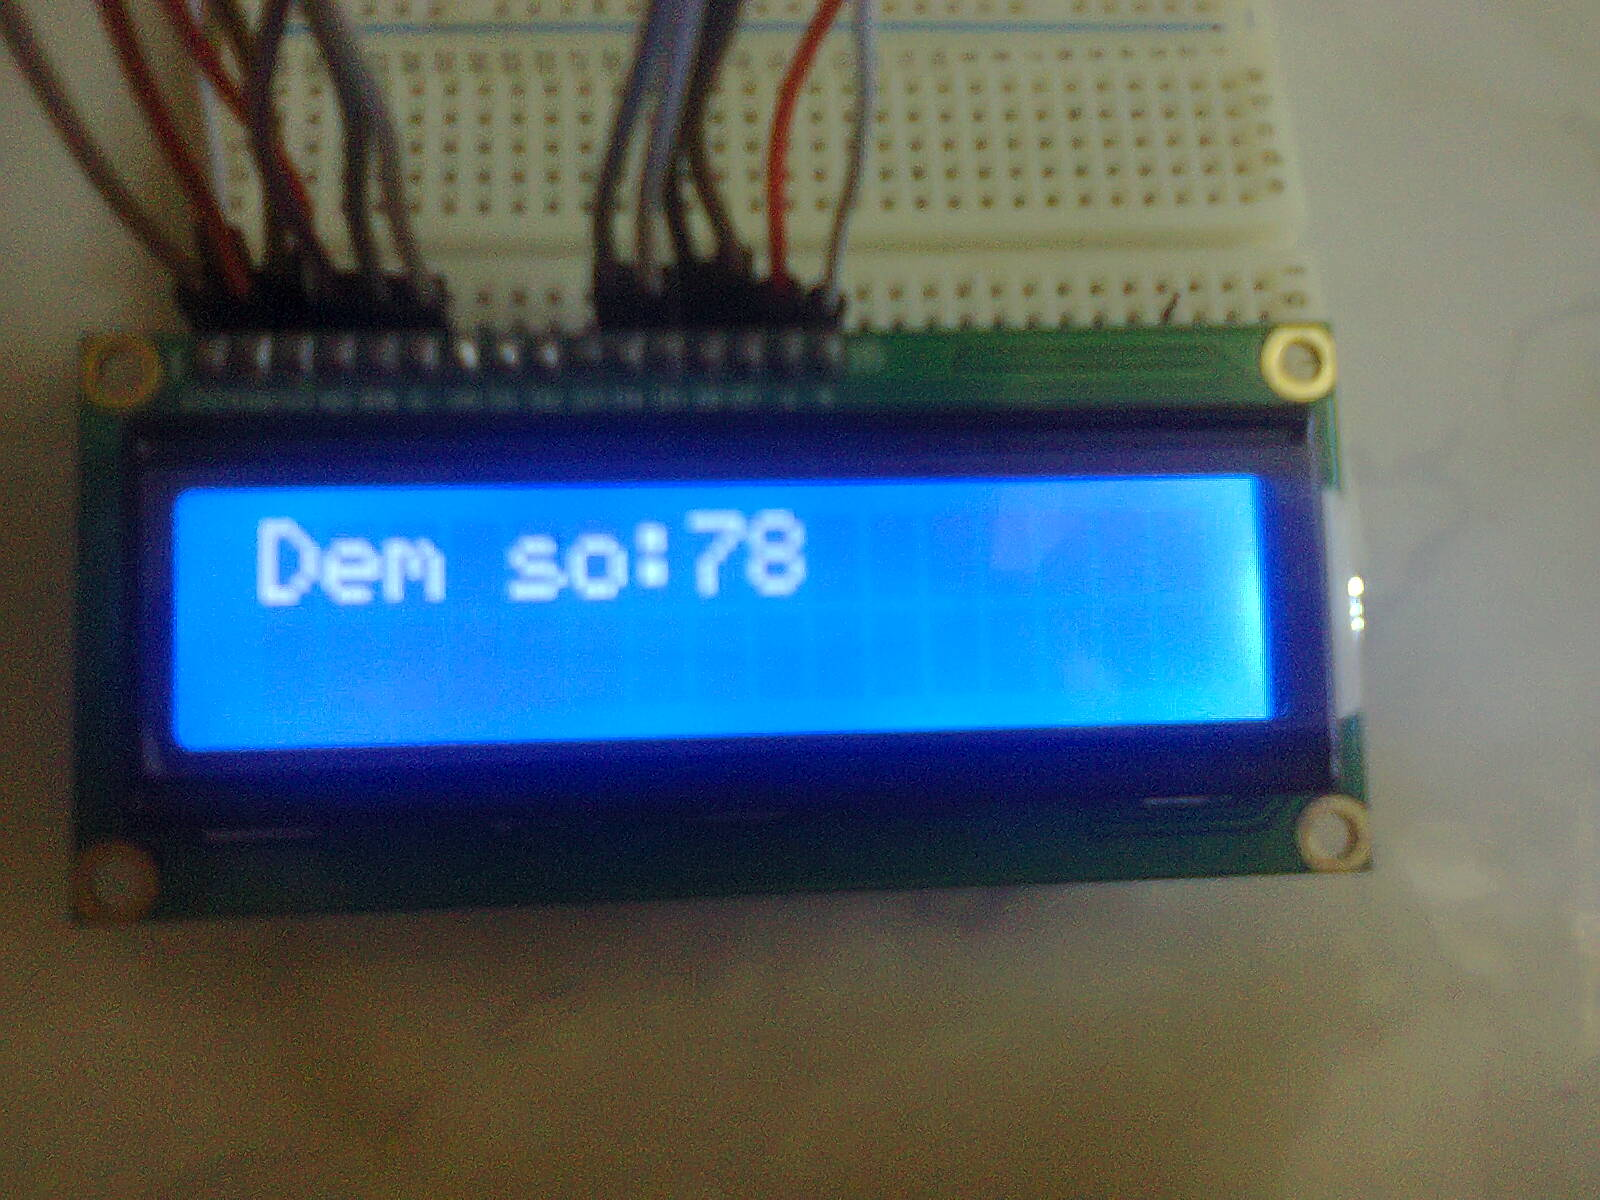
\includegraphics[width=.3\linewidth]{bai-2/image/2-3}}
\end{center}
\caption[]{Kết quả chương trình đếm số hiển thị lên LCD 16x02}
\end{figure}
\subsection*{Chương trình 6}
\lstinputlisting[language=C]{BAI-2-3.C}
\chapter{XỬ LÝ NGẮT}
\section{Giới thiệu chung}
\subsection{Yêu cầu}
Viết chương trình xử lý ngắt với nút nhấn.
\subsection{Hoạt động ngắt}
Ngắt là một tín hiệu điều khiển bắt vi điều khiển tạm ngưng công việc đang thực hiện để tiến hành các thao tác khác do ngắt quy đinh qua chương trình ngắt.

Khi phát hiện ngắt thì vi điều khiển sẽ thực hiện một chương trình độc lập với chương trình chính gọi là chương trình ngắt.\\

Cấu trúc của một chương trình ngắt:
\begin{itemize}
\item Bắt đầu là tên ngắt: \verb|#INT_tên_ngắt| với \verb|tên_ngắt| ta có thể xem trong chương trình CCS (trong \verb|View/Valid Interrupts|).
\item Kế tiếp là \emph{chương trình ngắt} (tùy theo mục đích mà chúng ta viết chương trình hoạt động khi xảy ra ngắt).
\begin{verbatim}
tên_hàm(){
    //Nội dung chương trình ngắt
}
\end{verbatim}
\end{itemize}
\section{Thiết lập hoạt động ngắt}\label{Sec:int}
Sử dụng các lệnh sau để thiết lặp hoạt động ngắt:
\begin{itemize}
\item \verb|ENABLE_INTERRUPTS(level);| với \verb|level| là \verb|INT_tên_ngắt| hoặc \verb|GLOBAL| (ngắt toàn cục): cho phép ngắt.
\item \verb|DISABLE_INTERRUPTS(level);| với \verb|level| giống như trên: vô hiệu hóa ngắt.
\item \verb|CLEAR_INTERRUPT(level);| với \verb|level| không có \verb|GLOBAL|: xóa cờ ngắt.
\item \verb|EXT_INT_EDGE(soure, edge);| với:
\begin{itemize}
\item \verb|soure = 0, 1, 2|: nguồn ngắt (ứng với \verb|EXT0|, \verb|EXT1|, \verb|EXT2|).
\item \verb|edge = L_TO_H, H_TO_L|: cạch kích ngắt (mức thấp lên cao hoặc mức cao xuống thấp).
\end{itemize}
\end{itemize}

Thiết kế chương trình có dùng ngắt:
\begin{itemize}
\item Trong hàm \verb|main()|: cho phép ngắt cụ thể (\verb|tên_ngắt|), ngắt toàn cục (\verb|GLOBAL|) và đợi ngắt (\verb|EXT_INT_EDGE|).
\item Chương trình xử lý ngắt (đặt trước hàm \verb|main()|): xóa cờ ngắt (\verb|CLEAR_INTERRUPT|), cấm ngắt toàn cục (\verb|DISABLE_INTERRUPTS(GLOBAL);|) xử lý chương trình ngắt xong rồi cho phép ngắt toàn cục lại (\verb|ENABLE_INTERRUPTS(GLOBAL);|)
\end{itemize}
\section{Bài tập}
\subsection{Bài tập 3.1}
\paragraph{Yêu cầu}Viết chương trình nhận nút nhấn ở chân B0 của PIC 16F887, cứ mỗi lần nhấn phím sẽ đảo trạng thái các LED ở PORT E.
\paragraph{Hướng giải quyết}
\begin{itemize}
\item Chân \verb|B0| cho phép ngắt ngoài, nên chúng ta sử dụng \verb|#INT_EXT|.
\item Chương trình ngắt: thiết kế như hướng dẫn ở \emph{mục \ref{Sec:int}}, nội dung ngắt là đảo trạng thái PORT E: \verb|PORTE =| $\sim$\verb|PORTE;|
\item Chương trình chính: 
\begin{itemize}
\item Khai báo \verb|PORT B| là chân \verb|INPUT| (nút nhấn): \verb|TRISB = 0xFF;| còn \verb|PORT E| là chân \verb|OUTPUT| (led): \verb|TRISE = 0x00;|
\item Ở \verb|PORT B| khi giao tiếp nút nhấn, cần có điện trở mắc lên nguồn cho chân B0, ta khai báo: \verb|PORT_B_PULLUPS(0x01);|
\item Kích hoạt ngắt ngoài: \verb|ENABLE_INTERRUPTS(INT_EXT);| 
\item Chọn cạnh ngắt: \verb|EXT_INT_EDGE(H_TO_L);| \item Kích hoạt ngắt toàn cục \verb|ENABLE_INTERRUPTS(GLOBAL);|
\item Duy trì hoạt động của vi điều khiển: dùng \verb|while|.
\end{itemize}
%\item[$\ast$] \textit{Lưu ý}: tùy vào phần cứng chúng ta thiết kế có thể sẽ bị nhiễu, dẫn đến xảy ra ngắt khi mới vào chương trình, nếu bị nhiễu thì chúng ta thay đổi trạng thái LED ở PORT E là: \verb|PORTE = 0x00| hoặc \verb|PORTE = 0xFF| để cho phù hợp.
\end{itemize}
\subsection*{Sơ đồ mạch}
\begin{figure}[!h]
\begin{center}
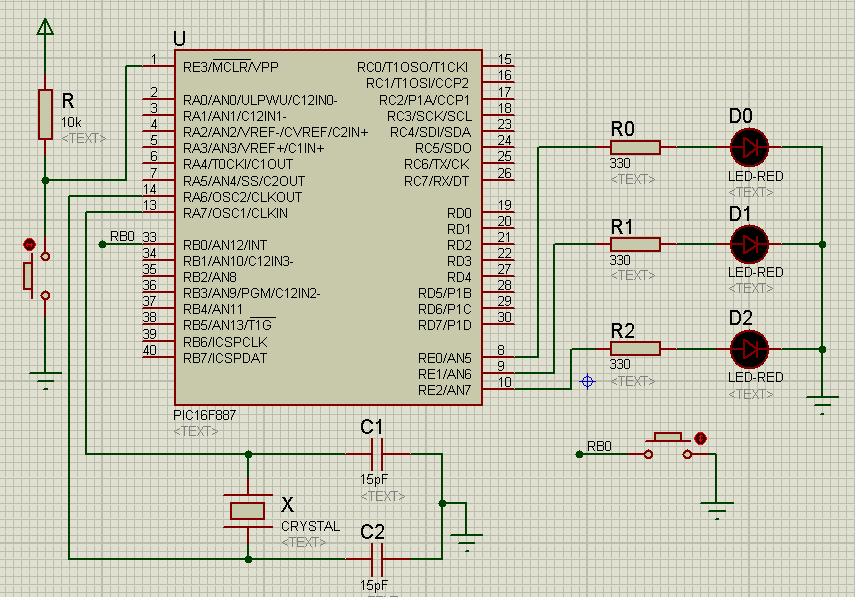
\includegraphics[scale=0.6]{bai-3/image/BAI-3-1}
\end{center}
\caption{Mạch đảo trạng thái LED ở PORT E với ngắt ngoài}
\end{figure}
\subsection*{Chương trình 7}
\lstinputlisting[language=C]{BAI-3-1.C}
\subsection{Bài tập 3.2}\label{Ex:3-2}
\paragraph{Yêu cầu}Viết chương trình hiển thị số lần nhấn phím ở chân B0 của PIC 16F887 lên màn hình LCD 16x02.
\paragraph{Hướng giải quyết}
\begin{itemize}
\item Sử dụng lại \emph{chương trình 7} với một số thay đổi như sau:
\begin{itemize}
\item Khai báo biến \verb|count| là biến toàn cục (để ảnh hưởng đến toàn chương trình).
\item Thay lệnh \verb|PORTE =| $\sim$\verb|PORTE| bằng lệnh \verb|count++|.
\end{itemize}
\item Trong chương trình chính ta thực hiện:
\begin{itemize}
\item Khai báo LCD (được trình bày trong \emph{chương trình 6} của \emph{bài tập 2.3}).
\item Sử dụng vòng lặp \verb|while| để duy trì chương trình: trong vòng lặp cho hiển thị biến \verb|count| lên LCD bằng hàm \verb|printf| kết hợp với hàm \verb|LCD_PutChar|.
\end{itemize}
\item Với các khai báo trên thì chương trình sẽ xảy ra nhiễu (do dội phím, rung do phần cứng), khi đó phải khắc phục nhiễu theo \textit{bài tập 3.4 trang \pageref{Ex:3-4}}.
\item[$\ast$] \textit{Lưu ý}: Khi chúng ta chưa xử lý chống nhiễu thì nó sẽ xảy ra một ngắt không mong muốn.
\item \textit{Hướng giải quyết khác cho bài này}: Ta không dùng ngắt, mà thay vào đó dùng hàm \verb|input(PIN_B0)| để đọc tín hiệu từ nút nhấn. Rồi xử lý chống nhiễu bằng cách thêm hàm \verb|delay_ms(500)| vào lệnh \verb|if| sau khi đọc được nút nhấn.
\item[$\ast$] Trong bài này chúng ta không sử dụng hàm \verb|input| trong \textit{chương trình chính} là do nội dung của bài thực hành là khảo sát ngắt trên vi điều khiển PIC 16F887, nên chọn hàm \verb|input| để sử dụng thì không hợp với nội dung.
\item[$\ast$] Để so sánh chương trình dùng ngắt và chương trình dùng \verb|input|, ta cùng xem chương trình trong \textit{mục \ref{Code:Button 3-2} trang \pageref{Code:Button 3-2}}.
\end{itemize}
\subsection*{Sơ đồ mạch}
\begin{figure}[!h]
\begin{center}
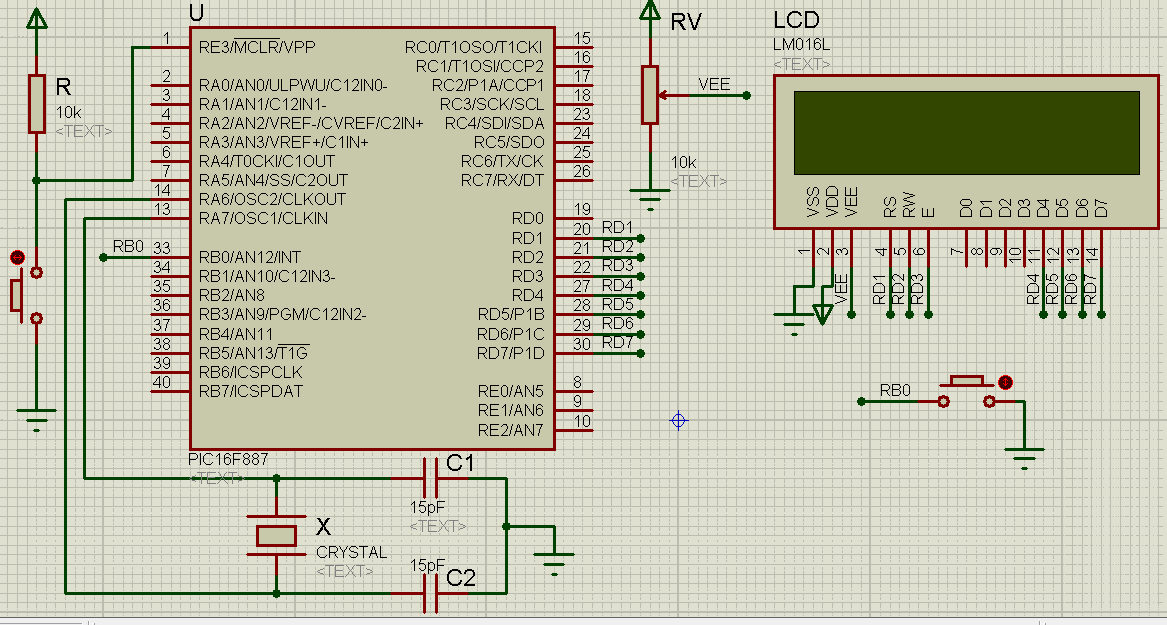
\includegraphics[scale=0.5]{bai-3/image/BAI-3-2}
\end{center}
\caption{Mạch đọc số lần nhấn nút ở chân B0 hiển thị lên LCD}
\end{figure}
\newpage
\subsection*{Chương trình 8}
\lstinputlisting[language=C]{BAI-3-2.C}
\newpage
\subsection{Bài tập 3.3}
\paragraph{Yêu cầu}Viết chương trình nhận nút nhấn ở chân \verb|B3 - B5| của PIC 16F887, hiển thị lên màn hình LCD 16x02.
\paragraph{Hướng giải quyết}
\begin{itemize}
\item Ở PIC 16F877A thì sử dụng các ngắt nối tiếp (từ chân RB4 -- RB7) dễ hơn nhiều so với PIC 16F887.
\item Để đơn giản, chúng ta không sử dụng ngắt nối tiếp mà dùng cách đọc tín hiệu từ các chân B3 -- B5 thông qua hàm input rồi cho xuất ra LCD.
\item Tạo một mảng: \verb|{B3, B4, B5} = {3, 4, 5}|, nếu nhấn nút nhấn ở chân B3 thì xuất ra biến \verb|kt = 3|, tương tự cho các chân còn lại.
\item Kiểm tra giá trị của biến \verb|kt| rồi cho xuất ra LCD thông qua hàm 

\verb|printf(LCD_PutChar)|.
\item Sử dụng điện trở nội cho các chân ở PORT B: \verb|PORT_B_PULL(0x38);| chỉ có 3 chân \verb|B3, B4, B5| được mắc trở lên nguồn.
\item[$\ast$] \textit{Kết luận}: Phần trên là ý tưởng giải quyết bài tập của em, nhưng khi chạy thực tế, vì lý do nào đó mà chân \verb|RB3| không lên mức cao được! Vấn đề này em chưa giải quyết được.
\end{itemize}
\subsection*{Sơ đồ mạch}
\begin{figure}[!h]
\begin{center}
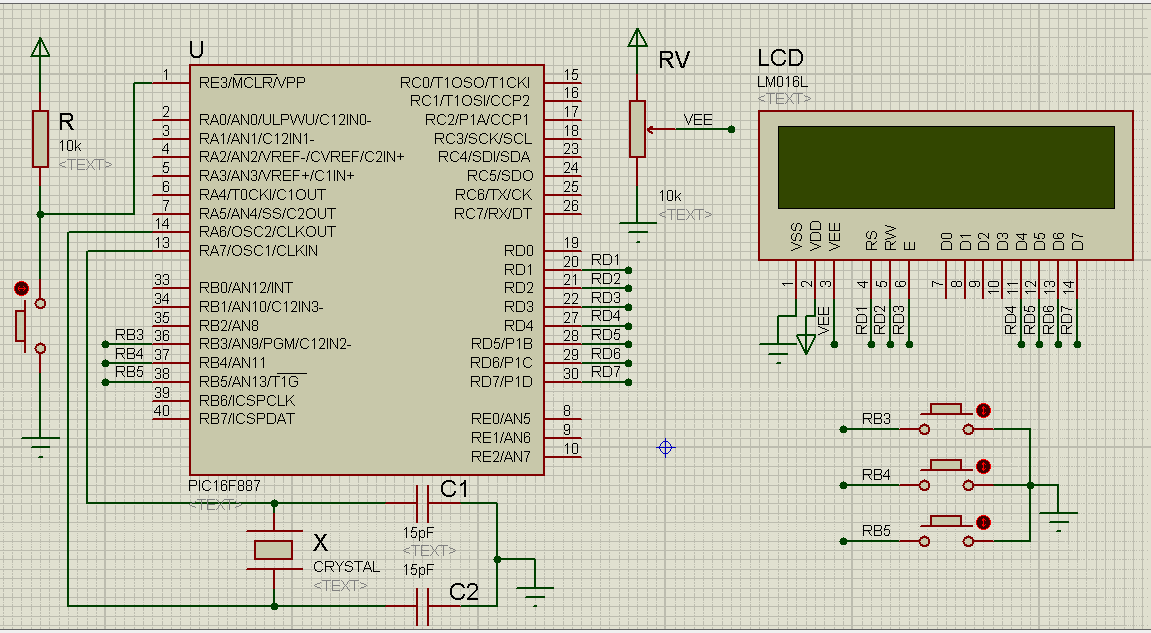
\includegraphics[scale=0.4]{bai-3/image/BAI-3-3}
\end{center}
\caption{Mạch đọc nút nhấn từ chân B3 -- B5 và hiển thị lên LCD}
\end{figure}
%\subsection*{Chương trình 9}
\subsection{Bài tập 3.4}\label{Ex:3-4}
\paragraph{Yêu cầu}Viết chương trình nhận nút nhất ở chân B0 của PIC 16F887 có xử lý chống nhiễu.
\paragraph{Hướng giải quyết}
\begin{itemize}
\item Khi sử dụng nút nhấn, có xảy ra quá trình dội, nhiễu và rung do phần cứng. Cụ thể là ở \emph{bài tập 3.1} khi ta nhấn nút thì LED bị nhiễu. Nên ta cần xử lý chống nhiễu cho tín hiệu.
\item Dùng hàm \verb|delay_ms(số mili giây)| với \verb|số mili giây = 10 - 20ms| để bỏ qua xung nhiễu. Rồi lấy mức 0 làm điều kiện có nút nhấn:

\verb|if input(PIN_B0) == 0| thì thực hiện lệnh cần thiết.
\end{itemize}
\subsection*{Chương trình 9}
\lstinputlisting[language=C]{BAI-3-4.C}
\subsection{Đọc tín hiệu từ nút nhấn với hàm INPUT}\label{Code:Button 3-2}
Nội dung file \verb|INPUT_BUTTON.C| (Một cách làm khác của \textit{bài tập 3.2} trang \pageref{Ex:3-2}).
\subsection*{Chương trình 10}
\lstinputlisting[language=C]{INPUT_BUTTON.C}
\chapter{XỬ LÝ ADC}
\section{Giới thiệu chung}
\subsection{Yêu cầu}
Đọc giá trị ADC từ biến trở.
\subsection{ADC}
PIC 16F887 có 2 PORT hổ trợ tính năng ADC là: PORT A và PORT E. Có thể đọc ADC ở chế độ $10$ bit $\left({0-1023}\right)$ hoặc $8$ bit $\left({0-255}\right)$ tùy mục đích sử dụng. Điện áp tham chiếu của bộ ADC thường là $5V$.
\subsection{Sơ đồ mạch}
\begin{figure}[!h]
\begin{center}
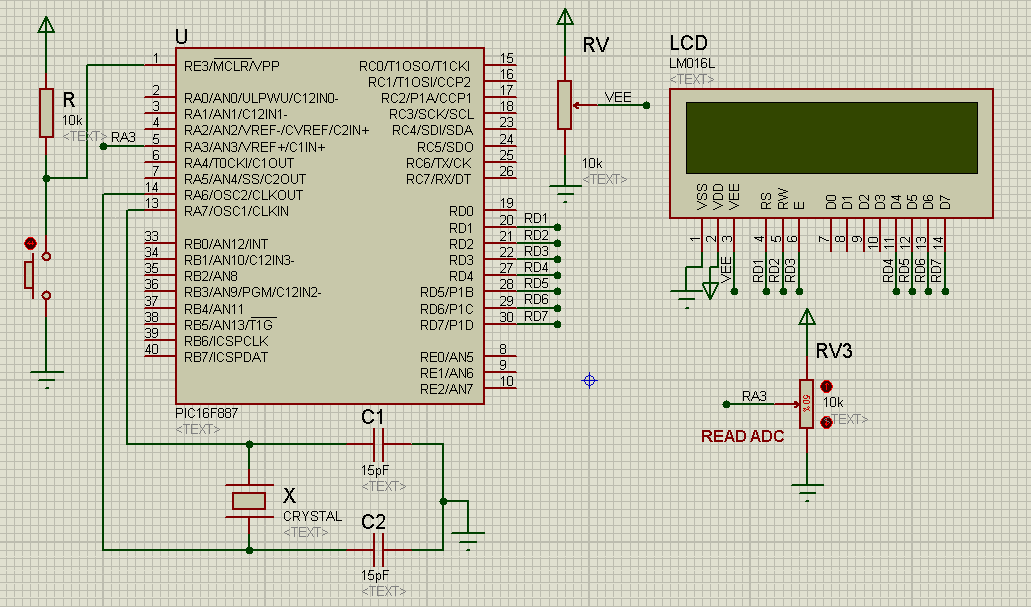
\includegraphics[scale=0.5]{bai-4/image/BAI-4-1}
\end{center}
\caption{Mạch đọc ADC từ biến trở}
\end{figure}
\section{Cấu hình ADC}
\begin{itemize}
\item Khai báo chế độ đọc ADC là $10$ hoặc $8$ bit:

\verb|#DEVICE *= 16 ADC 10| hoặc \verb|#DEVICE *= 16 ADC 8|
\item Xác định cách thức hoạt động của bộ biến đổi ADC: \verb|SETUP_ADC(mode);|
\item Xác định chân lấy tín hiệu ADC và điện thế sử dụng: \verb|SETUP_ADC_PORTS(value);|
%với giá trị của biến \verb|value| ta có thể tham khảo trong phần \verb|Help| của chương trình \verb|CSS|.
\item Chọn chân để đọc Analog với lệnh \verb|READ_ADC|, ta khai báo:

\verb|SET_ADC_CHANNEL(channel);| với \verb|channel| có giá trị từ $0 - 7$ theo tứ tự \verb|A0 - A5; E0 - E2|. Sau hàm này chúng ta nên dùng \verb|delay_us(10)| để cho kết quả đúng.
\item Đọc giá trị ADC từ chân đã khai báo ở hàm \verb|SET_ADC_CHANNEL| với lệnh \verb|READ_ADC(mode);| với \verb|mode| không bắt buộc.
\item[$\ast$] Các tham số (\verb|mode|, \verb|value| và \verb|channel|) của những hàm trên được định nghĩa trong thư mục \verb|DEVICES| ví dụ: \verb|16F887.h|, cách sử dụng những hàm này có thể xem trong phần \verb|Help| của phần mềm CCS.
\end{itemize}
\section{Bài tập}
\subsection{Bài tập 4.1}
\paragraph{Yêu cầu}Viết chương trình đọc giá trị ADC từ biến trở R7 và hiển thị lên LCD.
\paragraph{Hướng giải quyết}
\begin{itemize}
\item Khởi tạo LCD (trình bày trong \emph{chương trình 4 -- bài tập 2.1} của \emph{bài \ref{Les:LCD}}).
\item Cấu hình bộ ADC:
\begin{itemize}
\item Khai số bit đọc ADC, ta chọn \emph{10 bit}: \verb|#device *= 16 ADC 10|
\item Xác định hoạt động của bộ ADC, chọn \emph{thời gian lấy mẫu bằng xung clock}: \verb|SETUP_ADC(ADC_CLOCK_INTERNAL);|
\item Xác định chân đọc ADC, dùng \emph{chân A3}: \verb|SET_ADC_CHANNEL(3);| và \verb|delay_us(10)| (để bảo đảm giá trị đọc chính xác).
\end{itemize}
\item Thực hiện vòng lặp (dùng \verb|while|) đọc giá trị ADC (dùng \verb|READ_ADC|) và cho hiển thị giá trị lên LCD (dùng hàm \verb|printf| kết hợp với hàm \verb|LCD_PutChar|).
\end{itemize}
\newpage
\subsection*{Kết quả}
\begin{figure}[!h]
\vspace{-.5cm}
\begin{center}
  {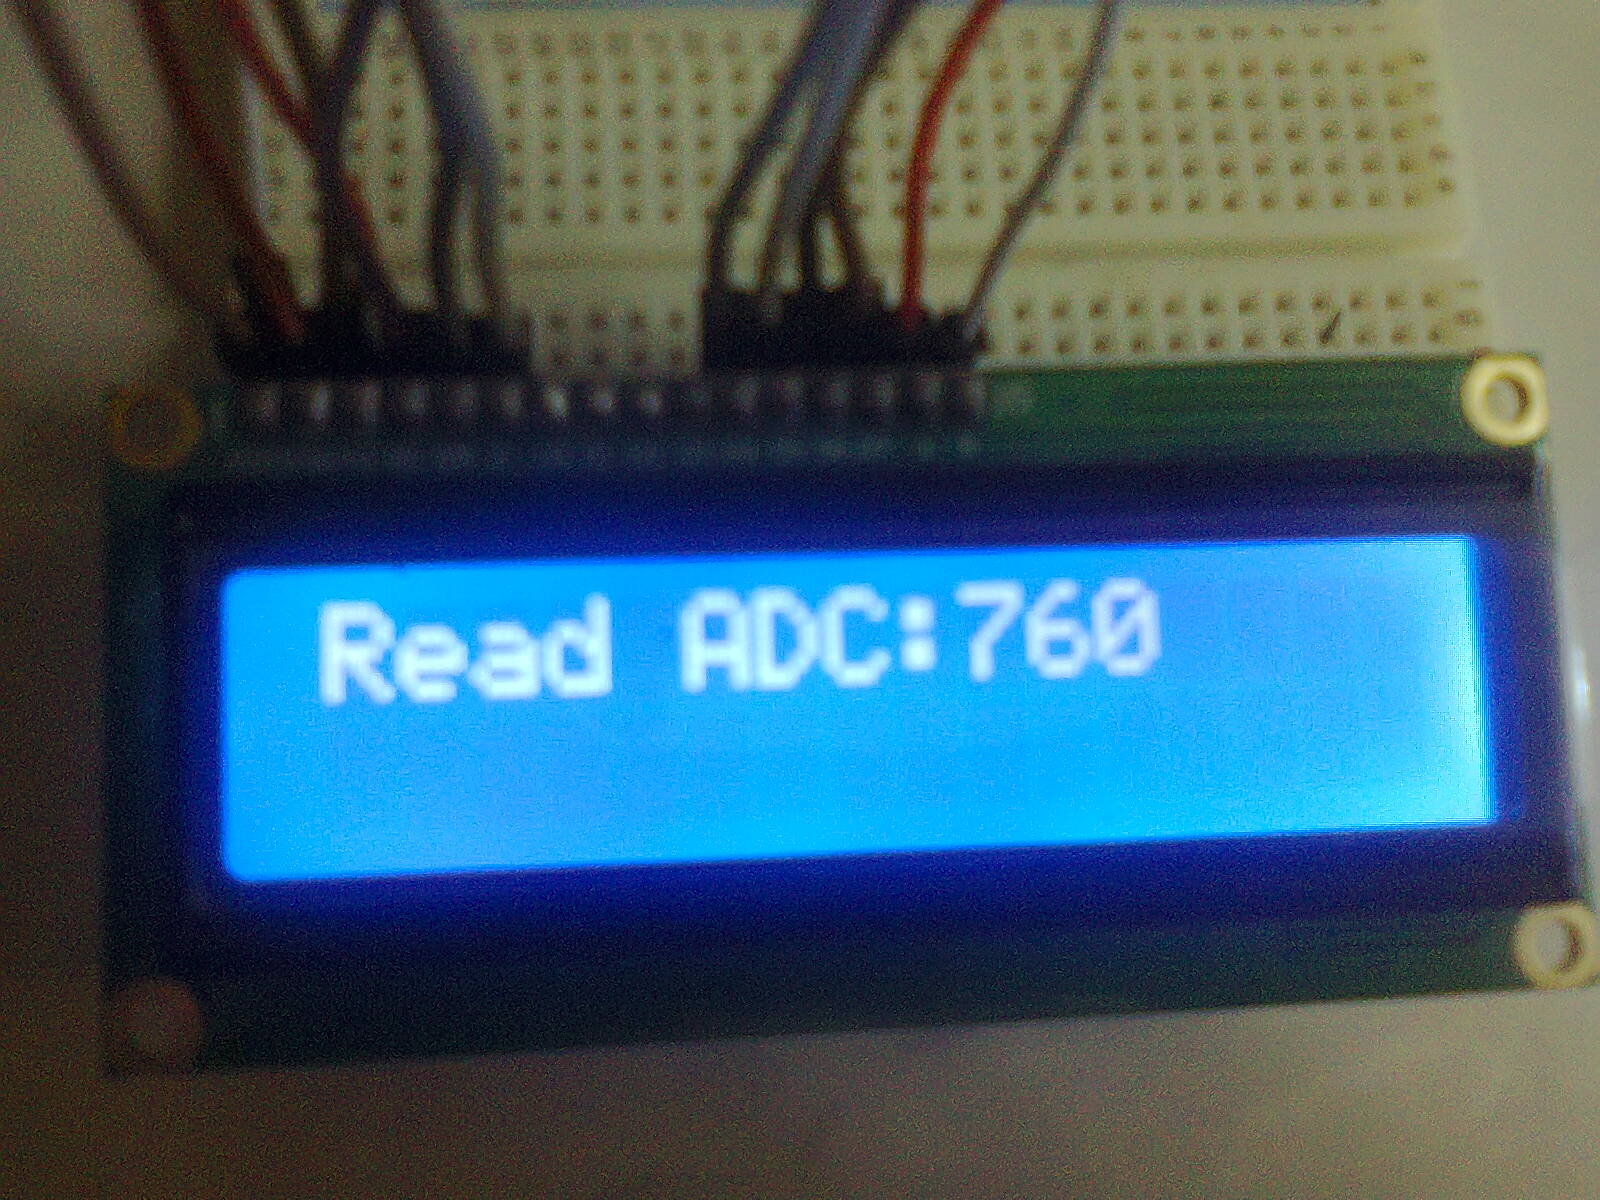
\includegraphics[width=.5\linewidth]{bai-4/image/4-1}}
\end{center}
\caption{Kết quả chương trình ADC hiển thị lên LCD 16x02}
\end{figure}
\subsection*{Chương trình 11}
\lstinputlisting[language=C]{BAI-4-1.C}
\subsection{Bài tập 4.2}
\paragraph{Yêu cầu}Viết chương trình đọc giá trị ADC từ biến trở R7 và xuất ra giá trị các LED ở \verb|PORT E|.
\paragraph{Hướng giải quyết}
\begin{itemize}
\item Đọc giá trị ADC như ở \textit{bài tập 4.1}.
\item Sau khi đọc được giá trị ADC từ biến trở, dùng hàm \verb|OUTPUT_E(value);| với \verb|value| là giá trị ADC đọc được.
\begin{itemize}
\item Giá trị ADC chúng ta đọc được trên LCD là ở dạng số nguyên, nên muốn hiểu rõ trạng thái của LED cần đổi giá trị ADC đọc được sang mã nhị phân.
\item Do \verb|PORT E| chỉ có 3 chân, nên chỉ quan tâm 3 số cuối của mã nhị phân.

Ví dụ: \verb|ADC = 511 = 0b01 1111 1111| (10 bit), chúng ta qua tâm số giá trị cuối của mã nhị phân là \verb|111|, khi đó cả 3 LED đều sáng.
\end{itemize}
\item Viết thêm lệnh chuyển từ số thập phân sang số nhị phân cho hiển thị lên LCD để dễ quan sát.
\end{itemize}
\newpage
\subsection*{Kết quả}
\begin{figure}[!h]
\begin{center}
  {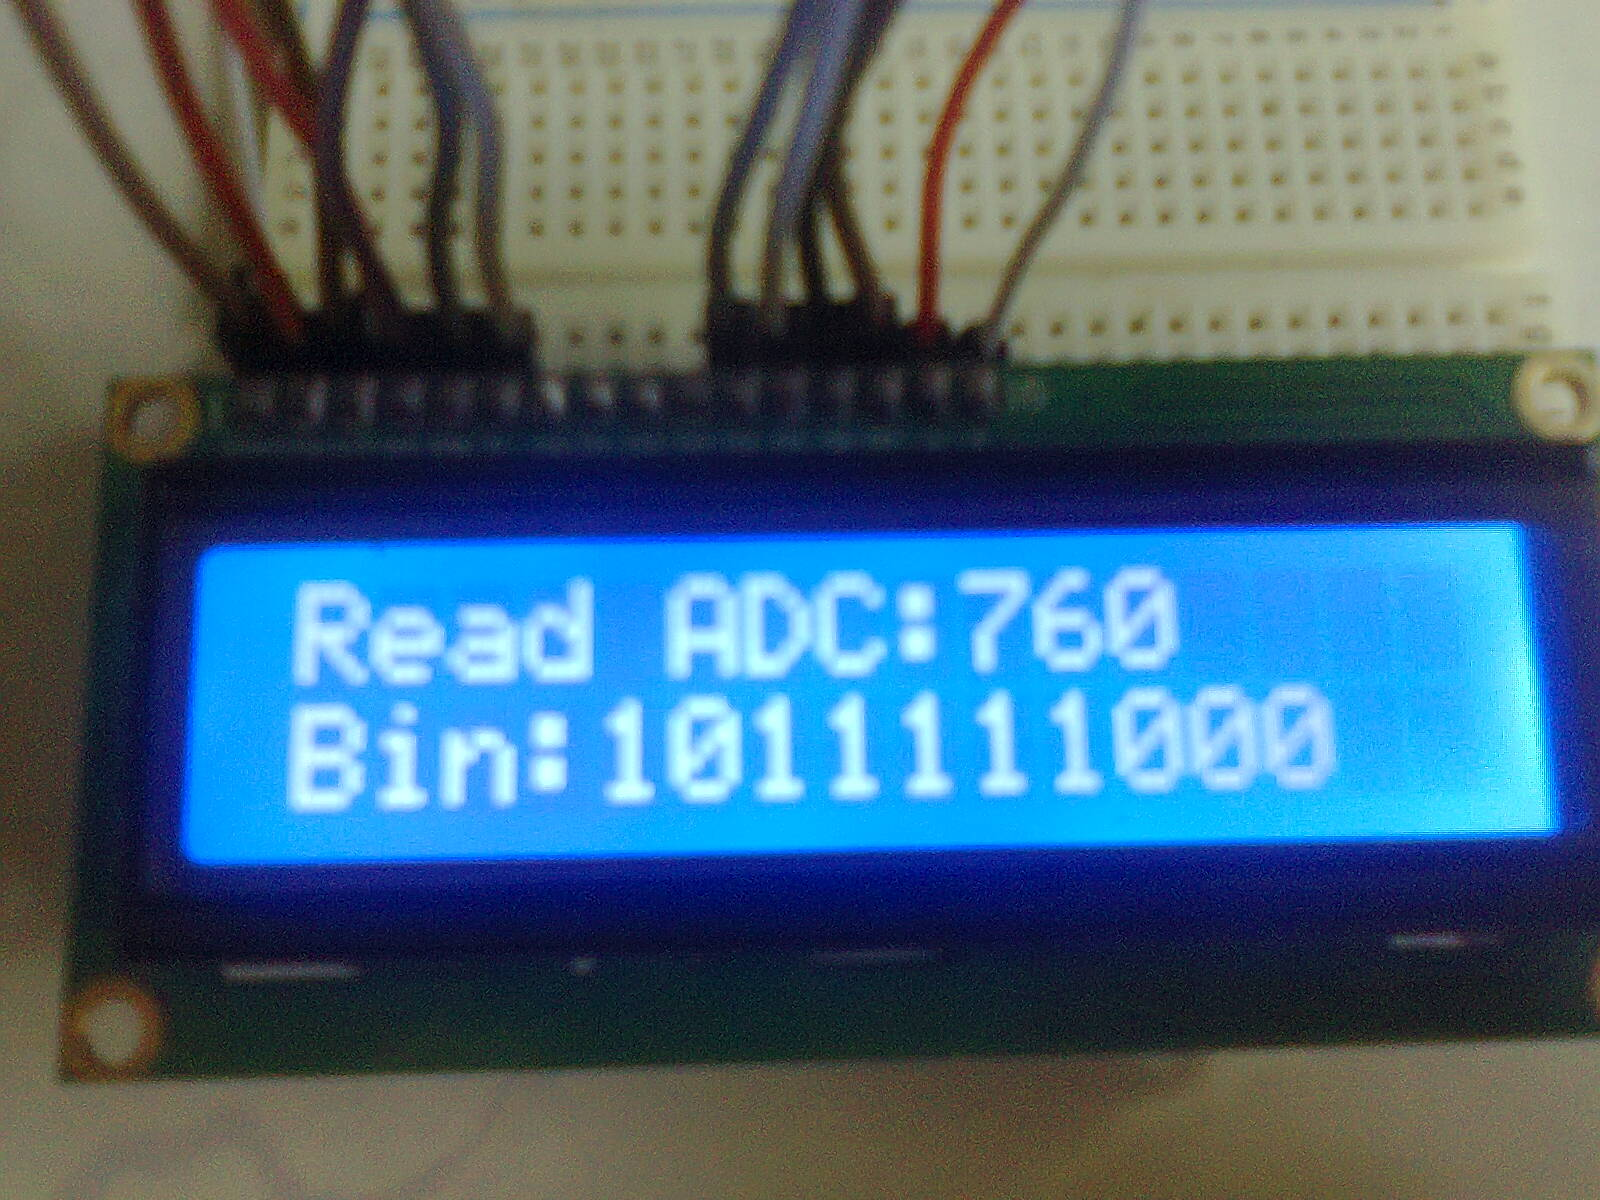
\includegraphics[width=.5\linewidth]{bai-4/image/4-2}}
\end{center}
\caption{Kết quả chương trình ADC xuất ra PORT E}
\end{figure}
\subsection*{Sơ đồ mạch}
\begin{figure}[!h]
\begin{center}
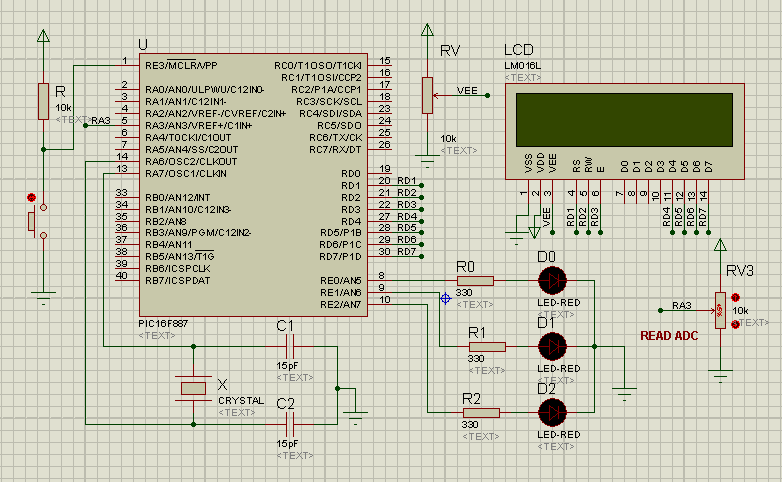
\includegraphics[scale=0.7]{bai-4/image/BAI-4-2}
\end{center}
\caption{Mạch đọc ADC từ biến trở xuất giá trị ra LED}
\vspace{1cm}
\end{figure}
\subsection*{Chương trình 12}
\lstinputlisting[language=C]{BAI-4-2.C}
\subsection{Bài tập 4.3}
\label{Ex:4-3}
\paragraph{Yêu cầu}Viết chương trình đọc ADC từ biến trở và gửi lên máy tính.
\paragraph{Hướng giải quyết}
\begin{itemize}
\item Phần code cho vi điều khiển:
\begin{itemize}
\item Để gửi dữ liệu từ vi điều khiển lên PC, chúng ta sử dụng chuẩn giao tiếp RS232 (được giới thiệu trong \textit{bài \ref{chapter:rs232} trang \pageref{chapter:rs232}}).
\item Thêm vào khai báo sau để giao tiếp RS232:

\verb|#use rs232(baud = 9600, xmit = PIN_C6, rcv = PIN_C7)|
\item Sau khi đọc được giá trị từ biến trở (giống như \textit{bài tập 4.1}), chúng ta gửi dữ liệu lên máy tính bằng lệnh: \verb|printf("%lu",adc)|.
\item Sử dụng lại \textit{chương trình 11} của \textit{bài tập 4.1} cho hiển thị lên LCD để kiểm chứng lại kết quả trên LCD và kết quả gửi lên máy tính.
\end{itemize}
\item Phần code cho Matlab\footnote{Tham khảo tại: http://www.picvietnam.com/forum/showthread.php?t=752}
\begin{itemize}
\item Dữ liệu do vi điều khiển gửi lên máy tính sẽ được lưu trong bộ nhớ đệm, để đọc giá trị từ bộ nhớ đệm ra ta phải thiết lập cho tham số \verb|BytesAvailableFcn|.
\item Khi có một byte được nhận ở bộ nhớ đệm thì tham số này sẽ được gọi.
\item Do đó cần viết hàm (hàm \verb|Serial_Callback| trong file \verb|Serial_Callback.m|) để đáp ứng sự kiện trên và cho hiển thị trực tiếp lên cửa sổ command line.
\end{itemize}
\end{itemize}
\paragraph{Sơ đồ mạch}{~\\}
\begin{figure}[!h]
\begin{center}
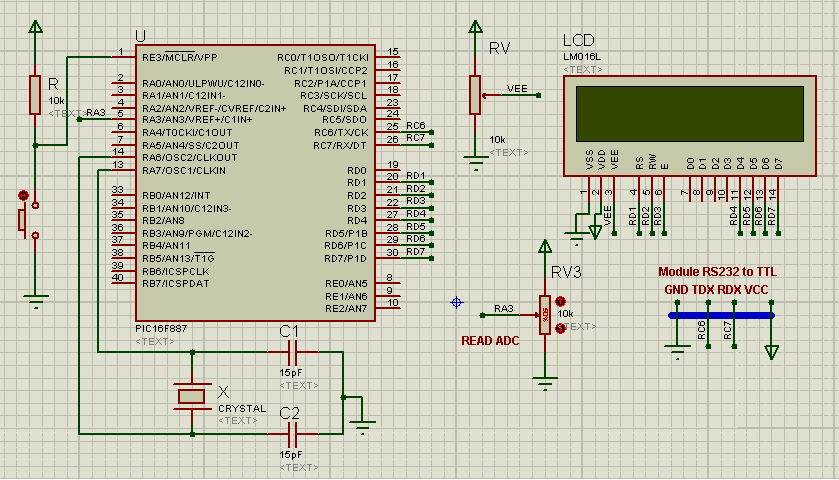
\includegraphics[scale=0.7]{bai-4/image/BAI-4-3}
\end{center}
\caption{Mạch đọc ADC từ biến trở gửi lên PC}
\end{figure}
\subsection*{Chương trình 13}
\lstinputlisting[language=C]{BAI-4-3.C}

Hàm \verb|Serial_Callback| dùng để thiết lập cho tham số \verb|BytesAvailableFcn| trước khi mở cổng COM:
\lstinputlisting[language=Matlab]{Serial_Callback.m}

Lệnh Matlab nhận dữ liệu từ vi điều khiển gửi lên:
\lstinputlisting[language=Matlab]{BAI-4-3.m}
\chapter{TIMER}
\section{Giới thiệu chung}
\subsection{Yêu cầu}
Sử dụng timer/counter trên vi điều khiển PIC 16F887 tạo thời gian trễ và tạo bộ đếm.
\subsection{Timer/Counter}
Timer được dùng để tạo ra khoảng thời gian trễ và nó cũng hoạt động như một bộ đếm (đếm số xung đi vào một chân cụ thể trên vi điều khiển).\\

Vi điều khiển PIC 16F887 có 3 bộ timer:
\begin{itemize}
\item \verb|Timer0|: $8$ bit, đếm được $255$, có chế độ định thời và bộ đếm.
\item \verb|Timer1|: $16$ bit, đếm được $65535$, có chế độ định thời và bộ đếm.
\item \verb|Timer2|: $8$ bit, có chức năng điều \verb|PWM| -- điều chế độ rộng xung.
\end{itemize}
\section{Các lệnh của Timer/Counter}
Gồm các lệnh sau:
\begin{itemize}
\item \verb|SETUP_TIMER_X(mode);| với \verb|X = 1| hoặc \verb|X = 2| (được định nghĩa trong \verb|device.h| (\verb|device| là tên chip)): khởi tạo \verb|TIMER|.
\item \verb|SET_TIMERx(value);| với \verb|x = 0| hoặc \verb|x = 1| hoặc \verb|x = 2|: thiết lặp giá trị bắt đầu cho \verb|TIMER|.
\item \verb|GET_TIMERx();| với \verb|x = 0| hoặc \verb|x = 1| hoặc \verb|x = 2|: đọc giá trị của \verb|TIMER/COUNTER|.
\end{itemize}

Xét cho từng bộ \verb|Timer|:
\begin{itemize}
\item \verb|TIMER0|: ta có các lệnh

\verb|SETUP_TIMER_0(mode);| \verb|SETUP_COUNTERS(rtcc_state, ps_state);| 

\verb|SET_TIMER0(value);| \verb|GET_TIMER0();|
\item \verb|TIMER1|: ta có các lệnh 

\verb|SETUP_TIMER_1(mode);| \verb|SET_TIMER1(value);| \verb|GET_TIMER1();|
\item \verb|TIMER2|: ta có các lệnh 

\verb|SETUP_TIMER_2(mode, period, postscale);| \verb|SET_TIMER2(value);| 

\verb|GET_TIMER2();|
\item[$\ast$] Các tham số (\verb|mode|, \verb|value|, \verb|rtcc_state|, \verb|ps_state|, \verb|period| và \verb|postscale|) của những hàm trên được định nghĩa trong thư mục \verb|DEVICES| ví dụ: \verb|16F887.h|, cách sử dụng những hàm này có thể xem trong phần \verb|Help| của phần mềm CCS.
\end{itemize}
\section{Bài tập}
\subsection{Bài tập 5.1}
\paragraph{Yêu cầu}Viết chương trình chớp tắt LED ở PORT E với thời gian delay $1s$ sửa dụng timer của PIC 16F887.
\paragraph{Hướng giải quyết}
\begin{itemize}
\item Đây là chương trình tạo thời gian trễ bằng cách sử dụng timer.
\item Chọn \verb|Timer0| $8$ bit để tạo thời gian trễ.
\item Tiến hành tính toán giá trị ban đầu cho thanh ghi \verb|TMR|: 
\begin{center}
\begin{tabular}{l|c|c|c|l|c}
\centering{Thông số} & Ký hiệu & Giá trị & Bộ chia & Giá trị &\verb|TMR0| \\ \hline
Tần số thạch anh & $F$ & $20MHz$ & $2$ & $2500$ & \\
Tần số lệnh & $\displaystyle F^\prime = \frac{F}{4}$ & $5MHz$ & $4$ & $1250$ &\\
Số xung trong $1s$ &  & $5 \times 10^6$ & $8$ & $625$ &\\
Số xung trong $1ms$ &  & $5 \times 10^3$ & $16$ & $312.5$ &\\
&  & & $32$ & $156.25$ & $256 - 156$\\
&  & & $64$ & $78.125$ &$= 100$\\
&  & & $128$ & $39.0625$ &\\
&  & & $256$ & $19.53125$ &\\
\end{tabular}
\end{center}
\begin{itemize}
\item Trong $1ms$ thực hiện $5 \times 10^3$ xung, mà \verb|Timer0| chỉ đếm được tới $255$. Nên chúng ta biến đổi số $5 \times 10^3$ qua các bộ chia trước.
\item Trong đó bộ chia trước $32$ là cho kết quả ít sai lệch so với các bộ chia khác. Chọn bộ chia $1:32$.
\item Thiết lập giá trị cho \verb|Timer0|: bộ \verb|Timer0| có $256$ giá trị, theo như cách chọn trên thì phải \verb|Timer0| phải đếm $156$ lần thì mới được $1ms$, nên cần phải cài đặt giá trị bắt đầu cho \verb|Timer0| là: $256 - 156 = 100$: \verb|SET_TIMER0(100);|
\end{itemize}
\item Sau khoảng thời gian đếm từ $100 \div 256$ thì \verb|Timer0| sẽ tràn, nên chúng ta sử dụng ngắt \verb|#INT_TIMER0| để xác định tràn trên \verb|Timer0|.
\item Để thời gian delay là $1s$, xác định số lần tràn như sau: $ count = 1 \times 1000$ lần.
\item Khai báo cho \verb|Timer0|: chọn xung kích nội và bộ chia trước $32$, giá trị ban đầu là $100$ rồi đếm lên, nên: \verb|SETUP_TIMER_0(RTCC_INTERNAL|$|$\verb|RTCC_DIV_32);| \verb|SET_TIMER0(100);|
\item Khai báo ngắt tràn trên \verb|Timer0|: \verb|ENABLE_INTERRUPTS(INT_TIMER0);| và thực hiện thiết kế chương trình ngắt như hướng dẫn ở \emph{mục \ref{Sec:int}} trong \emph{trang \pageref{Sec:int}}.
\item Chương trình ngắt: 
\begin{itemize}
\item Mỗi lần tràn \verb|Timer0| ta tăng biến \verb|count|.
\item So sánh biến \verb|count| với $1000$, nếu thỏa: \verb|count = 0;| và đảo trạng thái PORT E: \verb|PORTE =| $\sim$\verb|PORRTE|.
\end{itemize}
\item Thực hiện vòng lặp (dùng \verb|while|) để giữ cho vi điều kiển hoạt động.
\end{itemize}
\paragraph*{Sơ đồ mạch} Sơ đồ mạch giống sơ đồ mạch của \emph{bài tập 1.3} trong \emph{bài \ref{Les:1}}.
\subsection*{Chương trình 14}
\lstinputlisting[language=C]{BAI-5-1.C}
\subsection{Bài tập 5.2}
\paragraph{Yêu cầu}Viết chương trình đếm từ $0$ đến $9999$ sử dụng \verb|Timer| của \verb|PIC 16F887|, hiển thị trên \verb|LCD 16x02|.
\paragraph{Hướng giải quyết}
\begin{itemize}
\item Chúng ta sử dụng lại \emph{chương trình 14} để tạo thời gian trễ là \verb|sleep|, ví dụ trong chương trình khai báo \verb|int32 sleep = 500;| (tạo thời gian trễ $500ms$).
\item Chương trình ngắt: cứ sao một khoảng thời gian \verb|sleep| thì chúng ta tăng giá trị của biến \verb|dem| lên.
\item Chương trình chính: thêm vào vòng lặp \verb|while| công việc: hiện thị giá trị biến \verb|dem| lên \verb|LCD| (sử dụng hàm \verb|printf| kết hợp với hàm \verb|LCD_PutChar|). Thêm vào điều kiện so sánh, nếu vượt quá giới hạn, đặt lại biến \verb|dem = 0;|
\end{itemize}
\paragraph{Sơ đồ mạch}Giống sơ đồ mạch \emph{bài tập 2.3} trong \emph{bài \ref{Les:LCD}}.
\subsection*{Chương trình 15}
\lstinputlisting[language=C]{BAI-5-2.C}
\subsection{Bài tập 5.3}
\paragraph{Yêu càu}Viết chương trình đếm số lần nhấn phím sử dụng Timer của PIC 16F887, hiển thị trên LCD 16x02.
\paragraph{Hướng giải quyết}
\begin{itemize}
\item \verb|Timer 0| nhận được xung kích từ chân \verb|A4| của vi điều khiển (tùy thuộc vào cách ta cài đặt \verb|Timer 0|).
\item Cài đặt \verb|Timer 0|: \verb|SETUP_TIMER_0(RTCC_EXT_H_TO_L|$|$\verb|RTCC_DIV_1);| chọn bit cạnh xuống trên chân \verb|A4| và sử dụng bộ chia $1$ (do khi nhấn thì đếm và hiển thị lên \verb|LCD|, bộ chia $1$ là thích hợp nhất).
\item Cứ mỗi lần nhấn nút nhấn thì giá trị của \verb|Timer 0| tăng lên một giá trị. Sử dụng tính chất này để thực hiện đếm.
\item Thiết lập giá trị đầu cho \verb|Timer 0|: \verb|SET_TIMER0(0);| bắt đầu đếm từ 0.
\item Đọc giá trị của \verb|Timer 0|: \verb|value = GET_TIMER0();|. Chưa vội cho hiển thị giá trị \verb|value| lên LCD.
\item Do gặp phải vần đề sau: \verb|Timer 0| chỉ đếm được tới $255$, vượt quá $255$ thì chúng ta đếm sai, thực hiện kỹ thuật cộng dồn vào biến đếm: \verb|count = value + over*255|, với \verb|over| là số lần tràn (khi bắt đầu đếm thì \verb|over = 0;|)
\begin{itemize}
\item Chúng ta so sánh giá trị đọc được từ \verb|Timer 0| là biến \verb|value| với $255$ (giá trị tối đa của \verb|Timer 0|. Nếu \verb| value == 255| thì cho tăng biến \verb|over| lên.
\item Đồng thời cũng cần reset lại bộ đếm:\verb|SET_TIMER0(0);|
\end{itemize}
\item Phần còn lại, chúng ta chỉ việc cấu hình cho cho PORT A (chân \verb|INPUT|) và LCD rồi cho hiển thị giá trị của biến \verb|count| (đã thực hiện trong bài \ref{Les:LCD}).
\end{itemize}
\section*{Sơ đồ mạch}
\begin{figure}[!h]
\begin{center}
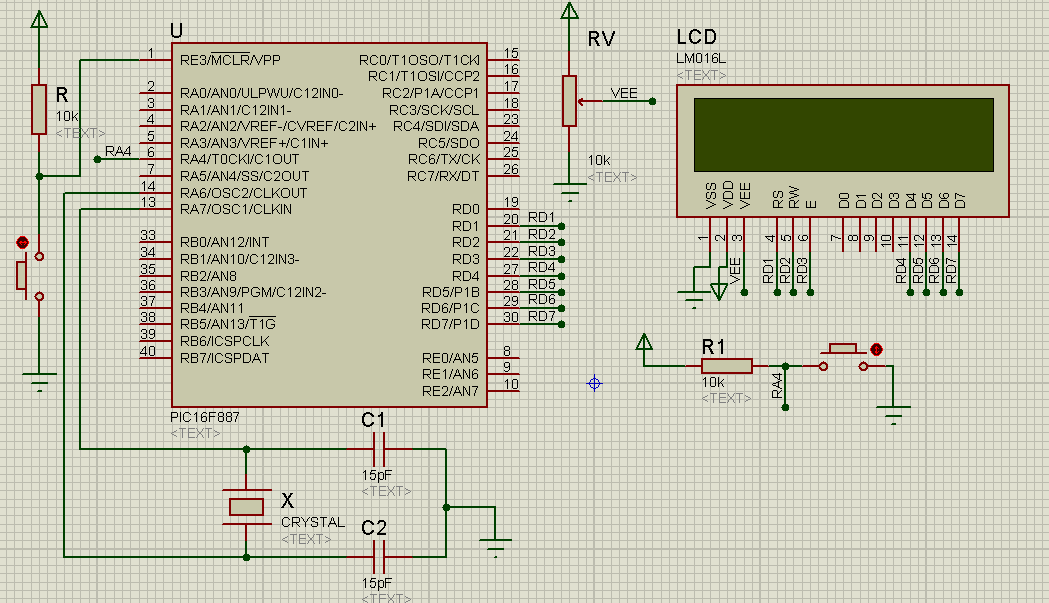
\includegraphics[scale=0.6]{bai-5/image/BAI-5-3}
\end{center}
\caption{Mạch đếm số lần nhấn nút sử dụng Timer hiển thị lên LCD}
\end{figure}
\newpage
\subsection*{Chương trình 16}
\lstinputlisting[language=C]{BAI-5-3.C}
\chapter{GIAO TIẾP I2C}
\section{Giới thiệu chung}
\subsection{Yêu cầu}Viết chương trình giao tiếp I2C giữa vi điều khiển PIC 16F887 với các module có chuẩn giao tiếp I2C.
\subsection{Chuẩn I2C}
Chuẩn I2C là chuẩn giao tiếp 2 dây là \verb|Serial Data (SDA)| (truyền dữ liệu 2 hướng) và \verb|Serial Clock (SCL)| (truyền xung đồng hồ theo một hướng).\\

Cách kết nối: chân \verb|SDA, SCL| của module lần lượt nối đến chân \verb|SDA, SCL| của vi điều khiển PIC 16F887. Ta có thể kết nối điều khiển nhiều thiết bị I2C với nhau thông qua 2 chân \verb|SDA| và \verb|SCL| của vi điều khiển. Mỗi thiết bị I2C sẽ được phân biệt bằng một \emph{địa chỉ duy nhất} \verb|address| hoặc \emph{quan hệ chủ tớ} \verb|master - slave|.
\section{Giao tiếp chuẩn I2C với CCS}
Để giao tiếp ta dùng khai báo và các lệnh sau:
\begin{itemize}
\item Khai báo: \verb|#use I2C(mode, speed, SDA = PIN_C4, SLC = PIN_C3)|, với:
\begin{itemize}
\item \verb|mode|: \verb|master| hoặc \verb|slave|.
\item \verb|speed|: \verb|slow| $\left({100kHz}\right)$ hoặc \verb|fast| $\left({400kHz}\right)$.
\item Trên PIC 16F887, chân \verb|C4| và chân \verb|C3| lần lượt là chân \verb|SDA| và \verb|SCL|.
\end{itemize}
\item Các hàm giao tiếp được CCS định nghĩa:
\begin{itemize}
\item \verb|I2C_ISR_STATE()|: Thông báo trạng thái giao tiếp I2C.
\item \verb|I2C_START()|: Tạo điều kiện \verb|START|.
\item \verb|I2C_STOP()|: Tạo điều kiện \verb|STOP|.
\item \verb|I2C_READ(mode)|: Đọc giá trị \verb|8 bit| thiết bị I2C. Với \verb|mode = 0| (không chỉ ra \verb|ACK|) và \verb|mode = 1| (chỉ ra \verb|ACK|)
\item \verb|I2C_WRITE(Device_address)|: Ghi giá trị \verb|8 bit| đến thiết bị I2C.
\end{itemize}
\item[$\ast$] Để hiểu rõ hơn các hàm này, có thể xem trong phần \verb|Help| của CCS.
\end{itemize}
\section{Bài tập}
\subsection{Bài tập 6.1}\label{Ex:6-1}
\paragraph{Yêu cầu}Viết chương trình đọc giá trị nhiệt độ từ cảm biến nhiệt TC 47 và hiển thị lên LCD 16x02.
\paragraph{Hướng giải quyết}
\begin{itemize}
\item Xác định chế độ truyền là \verb|Master| (quan hệ chủ -- tớ $\longleftrightarrow$ PIC (chủ) -- TC74 (tớ)).
\item Xác định địa chỉ của thiết bị I2C TC74 là: \verb|0x48| (Do thiết bị thực tập là TC74A0-5.0VAT, tùy dòng IC mà chúng ta xác định địa chỉ cho thích hợp, \textit{tham khảo trang 9 của datasheet \footnote{http://www.alldatasheet.com/} TC74}). %thêm số 0 vào cuối 7 bit trong trang 9 để được địa chỉ của thiết bị TC74).
\item Để giao tiếp với ngoại vi chuẩn I2C theo quan hệ chủ tớ, ta thực hiện như sau:
\begin{itemize}
\item Thiết bị chủ (PIC) tạo điều kiện \verb|Start|: \verb|i2c_start();|
\item Thiết bị chủ gửi địa chỉ của thiết bị tớ cùng với 1 bit 0, tức là gửi địa chỉ \verb|0x90| (\verb|0x48 = 1001000|, thêm bit 0 vào cuối: \verb|1001000 0 = 0x90|), dùng lệnh: \verb|i2c_write(0x90);| và đợi xung \verb|ACK| phản hồi từ thiết bị tớ (phần này đã giải thích tại sao phải thêm số 0 vào cuối 7 bit địa chỉ ở ý trên).
\item Khi thiết bị tớ đã nhận được đúng địa chỉ của nó (phản hồi xung \verb|ACK|), thiết bị chủ gửi lệnh thông báo truy cập vào thanh ghi đọc nhiệt độ - lệnh \verb|00h|, dùng lệnh: \verb|i2c_write(0x00);| (phần lệnh của TC74 được mô tả ở trang 8 trong datasheet).
\item Ta đã hoàn thành việc \textit{gửi yêu cầu đọc nhiệt độ} từ thiết bị tớ -- TC74, tiếp theo là thiết bị chủ (PIC) sẽ \textit{đọc giá trị nhiệt độ} từ thiết tớ (TC74).
\item Tạo lại điều kiện \verb|Start| để thực hiện giao tiếp mới: \verb|i2c_start();|
\item Thiết bị chủ gửi địa chỉ của thiết bị tớ cùng với bit 1 (lấy địa chỉ thiết bị I2C thêm vào bit 1: \verb|1001000 1 = 0x91|), dùng lệnh: \verb|i2c_write(0x91);|
\item Phần còn lại là đọc giá trị nhiệt độ từ thiết bị tớ, thiết bị chủ gửi xung \verb|Not-ACK| dùng lệnh: \verb|i2c_read(0);| (giá trị là số nguyên 8 bit).
\item Tạo điều kiện \verb|Stop|: \verb|i2c_stop();| để kết thúc quá trình giao tiếp.
\item Để giao tiếp được nhiều lần, ta thực hiện vòng lặp \verb|while| để lặp lại quá trình này (từ lệnh \verb|i2c_start();| đến \verb|i2c_stop();|).
\end{itemize}
\item Chúng ta lấy được giá trị nhiệt độ từ cảm biến TC74 và gửi lên LCD để quan sát.
\item Phần mô phỏng chương trình với phần mềm Protues em trình bày trong phần \textit{phục lục trang \pageref{def:TC74}}.
\item[$\ast$] Khi làm phần cứng, cần mắc thêm 2 điện trở \verb|pullup| lên nguồn.
\item[$\ast$] Ngoài cách giải thích trên, chúng ta có thể tham khảo cách giải thích khác trong phần chú thích \ref{note:TC74} ở bên dưới\footnote{http://embedded-lab.com/blog/using-tc74-microchip-thermal-sensor-for-temperature-measurement/\label{note:TC74}}.
\end{itemize}
\section*{Sơ đồ mạch}
\begin{figure}[!h]
\begin{center}
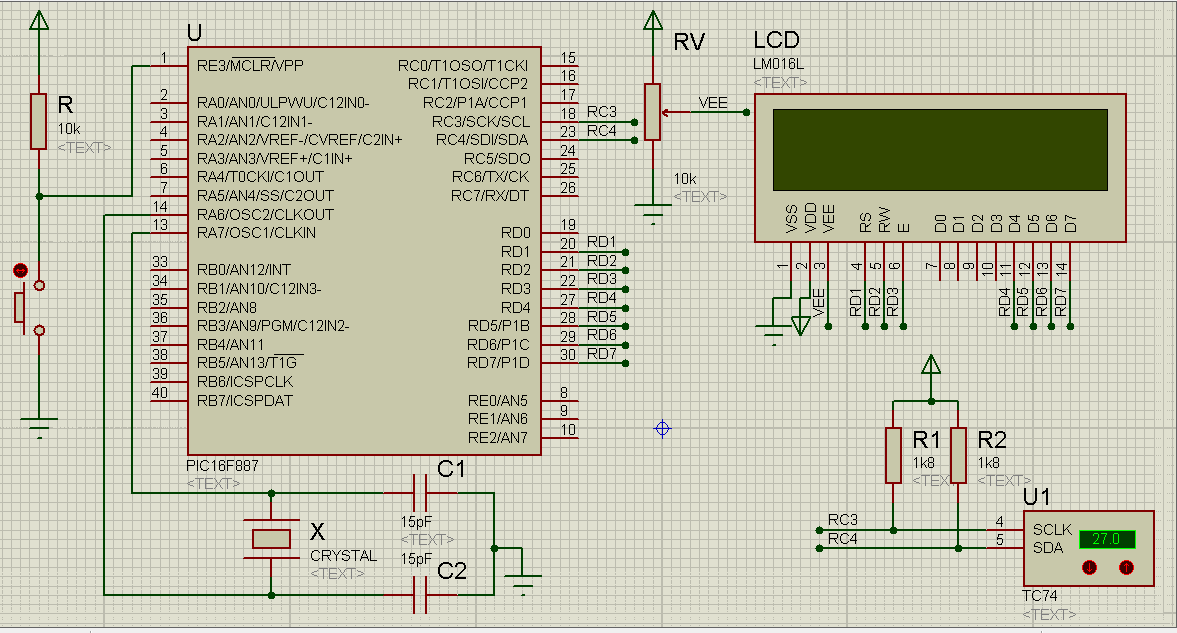
\includegraphics[scale=0.45]{bai-6/image/BAI-6-1}
\end{center}
\caption{Mạch đọc giá trị nhiệt độ từ IC TC74}
\end{figure}
\newpage
\subsection*{Chương trình 17}
\lstinputlisting[language=C]{BAI-6-1.C}
\subsection{Bài tập 6.2}
\label{Ex:ds3231-1}
\paragraph{Yêu cầu}Viết chương trình đọc giá trị thời gian từ IC DS1307 và hiển thị lên LCD 16x02.
\paragraph{Hướng giải quyết}Do không có IC DS1307 nên em thay thế bằng phần cứng khác là module RTC DS3231.
\begin{itemize}
\item[$\ast$] So với IC DS1307 thì IC DS3231 có thời gian chạy chính xác hơn. Module RTC DS3231 ngoài chức năng lấy thời gian thực, nó còn chức năng đo được giá trị nhiệt độ.
\item Chúng ta quan tâm đến các địa chỉ sau:
\begin{itemize}
\item Địa chỉ của thiết bị I2C là \verb|0x68|.
\item Địa chỉ của các thanh ghi lưu giá trị thời gian:
\begin{table}[!h]
\begin{center}
\begin{tabular}{|l|c|l|c|}\hline
\textit{Thanh ghi} & \textit{Địa chỉ} & \textit{Thanh ghi} & \textit{Địa chỉ}\\ \hline
\verb|secondREG| & \verb|0x00| & \verb|dayREG| & \verb|0x03| \\ \hline
\verb|minuteREG| & \verb|0x01| & \verb|dateREG| & \verb|0x04| \\ \hline
\verb|hourREG| & \verb|0x02| & \verb|monthREG| & \verb|0x05| \\ \hline
& & \verb|yearREG| & \verb|0x06| \\ \hline
\end{tabular}
\end{center}
\caption{Địa chỉ thanh ghi thời gian của IC DS3231}
\end{table}
\item Cài đặt định dạng thời gian hiển thị:
\begin{table}[!h]
\begin{center}
\begin{tabular}{|c|c|c|c|}\hline
\textit{Định dạng} & \textit{Cài đặt} & \textit{Định dạng} & \textit{Cài đặt} \\ \hline
\verb|_24_hour_format| & \verb|0| & \verb|am| & \verb|0| \\ \hline
\verb|_12_hour_format| & \verb|1| & \verb|pm| & \verb|1| \\ \hline
\end{tabular}
\end{center}
\caption{Cài đặt định dạng thời gian hiển thị}
\end{table}
\end{itemize}
\item Giá trị lưu trong thanh ghi ở dạng \verb|BCD|. Nên muốn ghi giá trị vào thanh ghi cần chuyển sang mã \verb|BCD|.
\item Sử dụng chương trình \verb|DS3231 High Precision I2C RTC Driver| do tác giả \verb|sshahryiar| trên diễn đàn \verb|https://www.ccsinfo.com|\footnote{https://www.ccsinfo.com/forum/viewtopic.php?t=50256} viết để làm bài này.
\begin{itemize}
\item Về thư viện chương trình gồm có 2 file: \verb|DS3231.h| và \verb|DS3231.C| (nội dung của các file trong phần phụ lục trang \pageref{def:DS3231}, do trong bài viết tác giả \verb|sshahryiar| không giải thích nội dung code, gây khó cho việc theo dõi, nên trong phần phụ lục em xin giải thích lại cách làm của tác giả để tiện cho việc theo dõi).
\item Với file \verb|DS3231.h| chứa định nghĩa các địa chỉ thanh ghi, cách định dạng thời gian và các hàm trong file \verb|DS3231.C|.
\item Chúng ta quan tâm đến việc sử dụng các hàm trong thư viện do tác giả \verb|sshahryiar| viết:
\begin{itemize}
\item Đầu tiên cần cài đặt thời gian thực vào IC bằng 2 hàm sau: (do thời gian trong IC không đúng với thời gian thực hiện tại).
\begin{verbatim}
       setTime(hr, min, s, am_pm, hr_format);
       setDate(dy, dt, mt, yr);
\end{verbatim}
Ví dụ: Thời gian thực hiện tại là: \verb|10:30:00 AM Tus 19-04-2016|, khi đó ta cài đặt thời gian như sau:
\begin{verbatim}
       setTime(10, 30, 0, 0, _12_hour_format);
       setDate(3, 19, 4, 16);
\end{verbatim}
\textit{Giải thích ý nghĩa của các tham số}:
\begin{table}[!h]
\begin{center}
\begin{tabular}{|c|l|c|l|}\hline
\verb|setTime| & \textit{Giải thích} & \verb|setDate| & \textit{Giải thích} \\ \hline
\verb|hr| & Giờ: \verb|1-12| (\verb|12h|) & \verb|dy| & Thứ: \verb|1-7| \\ 
& hoặc \verb|00-23| (\verb|24h|) & & (từ chủ nhật đến thứ 7) \\ \hline
\verb|min| & Phút: \verb|00-59| & \verb|dt| & Ngày: \verb|01-31|\\ \hline
\verb|s| & Giây: \verb|00-59| & \verb|mt| & Tháng: \verb|01-12|\\ \hline
\verb|am_pm| & Giờ: \verb|0| hoặc \verb|1|  & \verb|yr| & Năm: \verb|00-99|\\ 
& với \verb|am - 0| hoặc \verb|pm - 1| & & \\ \hline
\verb|hr_format| & Giờ \verb|12|: \verb|_12_hour_format| & & \\
 & Giờ \verb|24|: \verb|_24_hour_format| & & \\ \hline
\end{tabular}
\end{center}
\caption{Giải thích các tham số cài đặt thời gian thực cho IC DS3231}\label{Tab:set-DS3231}
\end{table}
\item Đọc thời gian trong \verb|IC| ra, ta dùng 2 hàm sau:
\begin{verbatim}
       getTime(hr, min, s, am_pm, hr_format);
       getDate(dy, dt, mt, yr);
\end{verbatim}
Với các tham số kết quả ra tùy thuộc vào cách ta đã cài đặt tham số đầu vào theo định nghĩa trong \textit{bảng \ref{Tab:set-DS3231}}.
\end{itemize}
\item Do ta truyền tham số vào ở dạng số, nên muốn hiển thị thứ hoặc giờ \verb|am| hay giờ \verb|pm| thì ta có thể kết hợp với cấu trúc \verb|switch - case| để lựa chọn giá trị xuất ra.
\end{itemize}
\item Trong chương trình cần thêm vào \verb|#include<DS3231.C>| để thêm thư viện vào chương trình. Tương tự như các bài tập trước ta khai báo LCD và thực hiện vòng lặp \verb|while| để giữ chương trình.
\item Cách chạy chương trình để IC DS3231 tự động cặp nhật thời gian: chúng ta thực hiện qua 2 bước sau:
\begin{itemize}
\item \textit{Bước 1}: Chạy \textit{chương trình 18 -- 1} cài đặt thời gian thực vào IC. Sau lần chạy đầu tiên, ta rút nguồn ra, nạp \textit{chương trình 18 -- 2} vào IC.
\item \textit{Bước 2}: Chạy \textit{chương trình 18 -- 2} để lấy thời gian trong IC ra -- thời gian lúc này mới là thời gian thực. Đến đây, quá trình nạp xem như thành công.
\item[$\ast$] Thật ra ở \textit{bước 2} chúng ta chỉ chú thích đi 2 dòng cài đặt thời gian ban đầu vào IC, sau khi chạy lần đầu tiên, IC sẽ tính giờ từ thời điểm ta cài vào (trường hợp ngắt nguồn thì IC đã có nguồn Pin 3V giúp IC nhớ được giờ), nên cấp nguồn lại thì thời gian vẫn đúng với thời gian thực. Do đó \textit{chương trình 18 -- 1} và \textit{chương trình 18 -- 2} chỉ là một chương trình (do đó ta thấy ở \textit{chương trình 18 -- 1} có một số lệnh chưa cần đến, làm cho chương trình dài lên).
\end{itemize}
\end{itemize}
\subsection*{Sơ đồ mạch}
\begin{figure}[!h]
\begin{center}
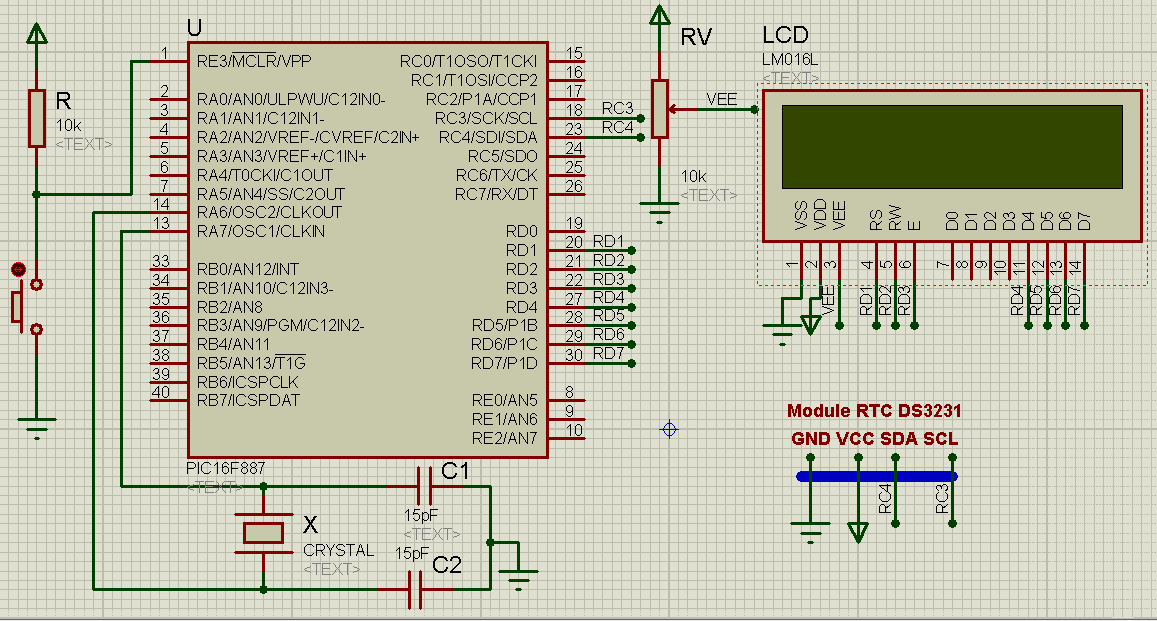
\includegraphics[scale=0.5]{bai-6/image/BAI-6-2}
\end{center}
\caption{Mạch đọc thời gian thực từ module RTC DS3231}
\end{figure}
\section*{Kết quả}
\begin{figure}[!h]
\begin{center}
%\subfloat[Sơ đồ mạch]
  {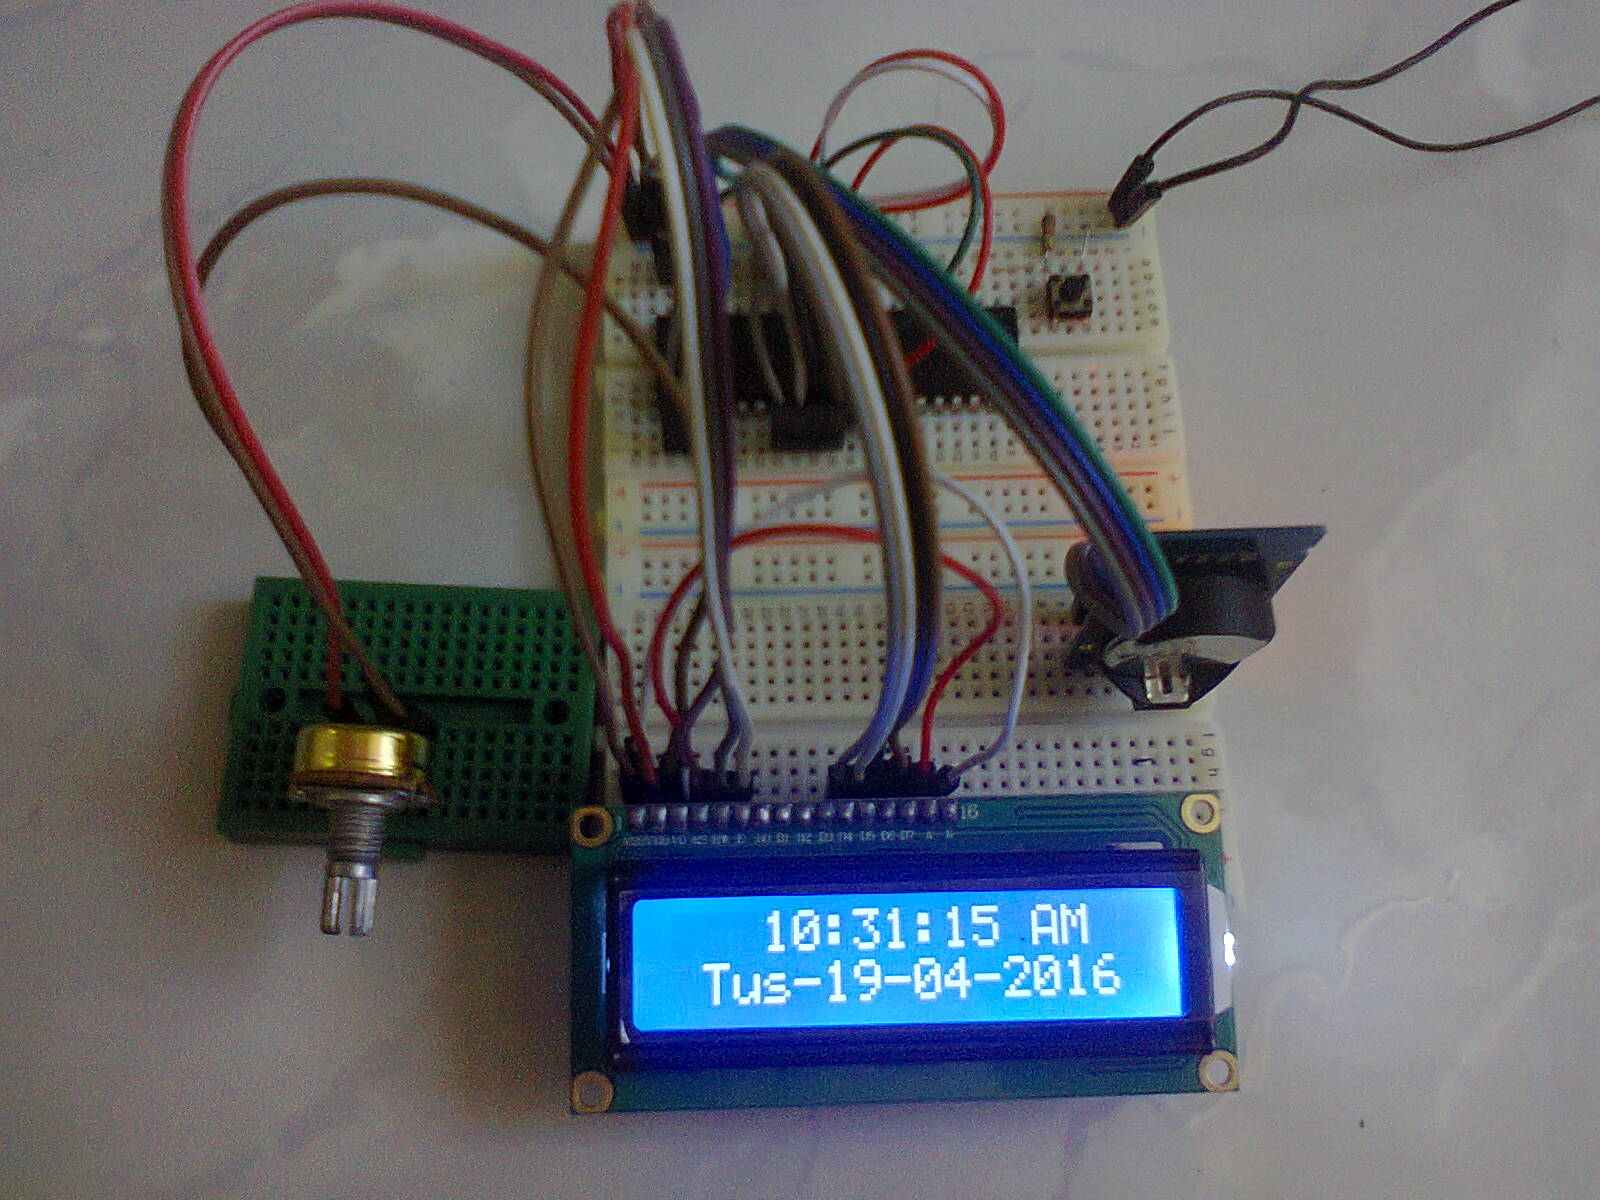
\includegraphics[width=.3\linewidth]{bai-6/image/6-2-1}}
%\subfloat[Kết quả]
  {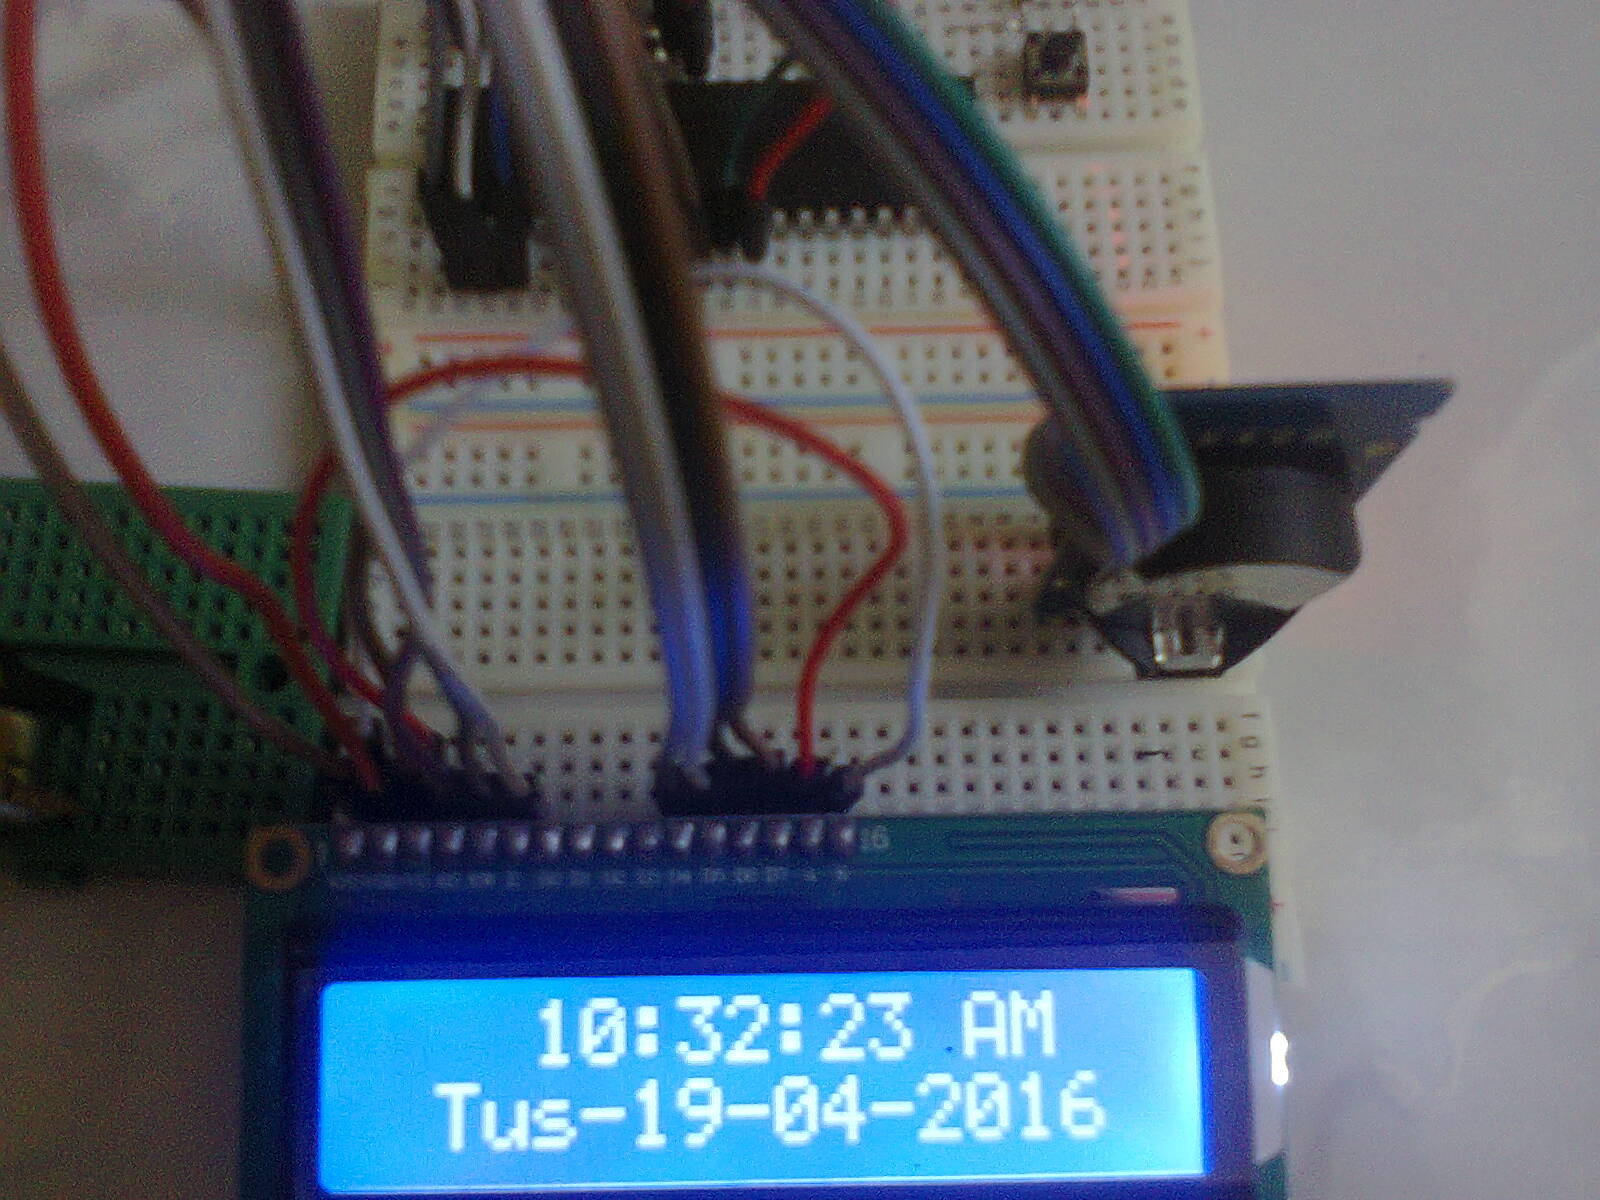
\includegraphics[width=.3\linewidth]{bai-6/image/6-2-2}}
  {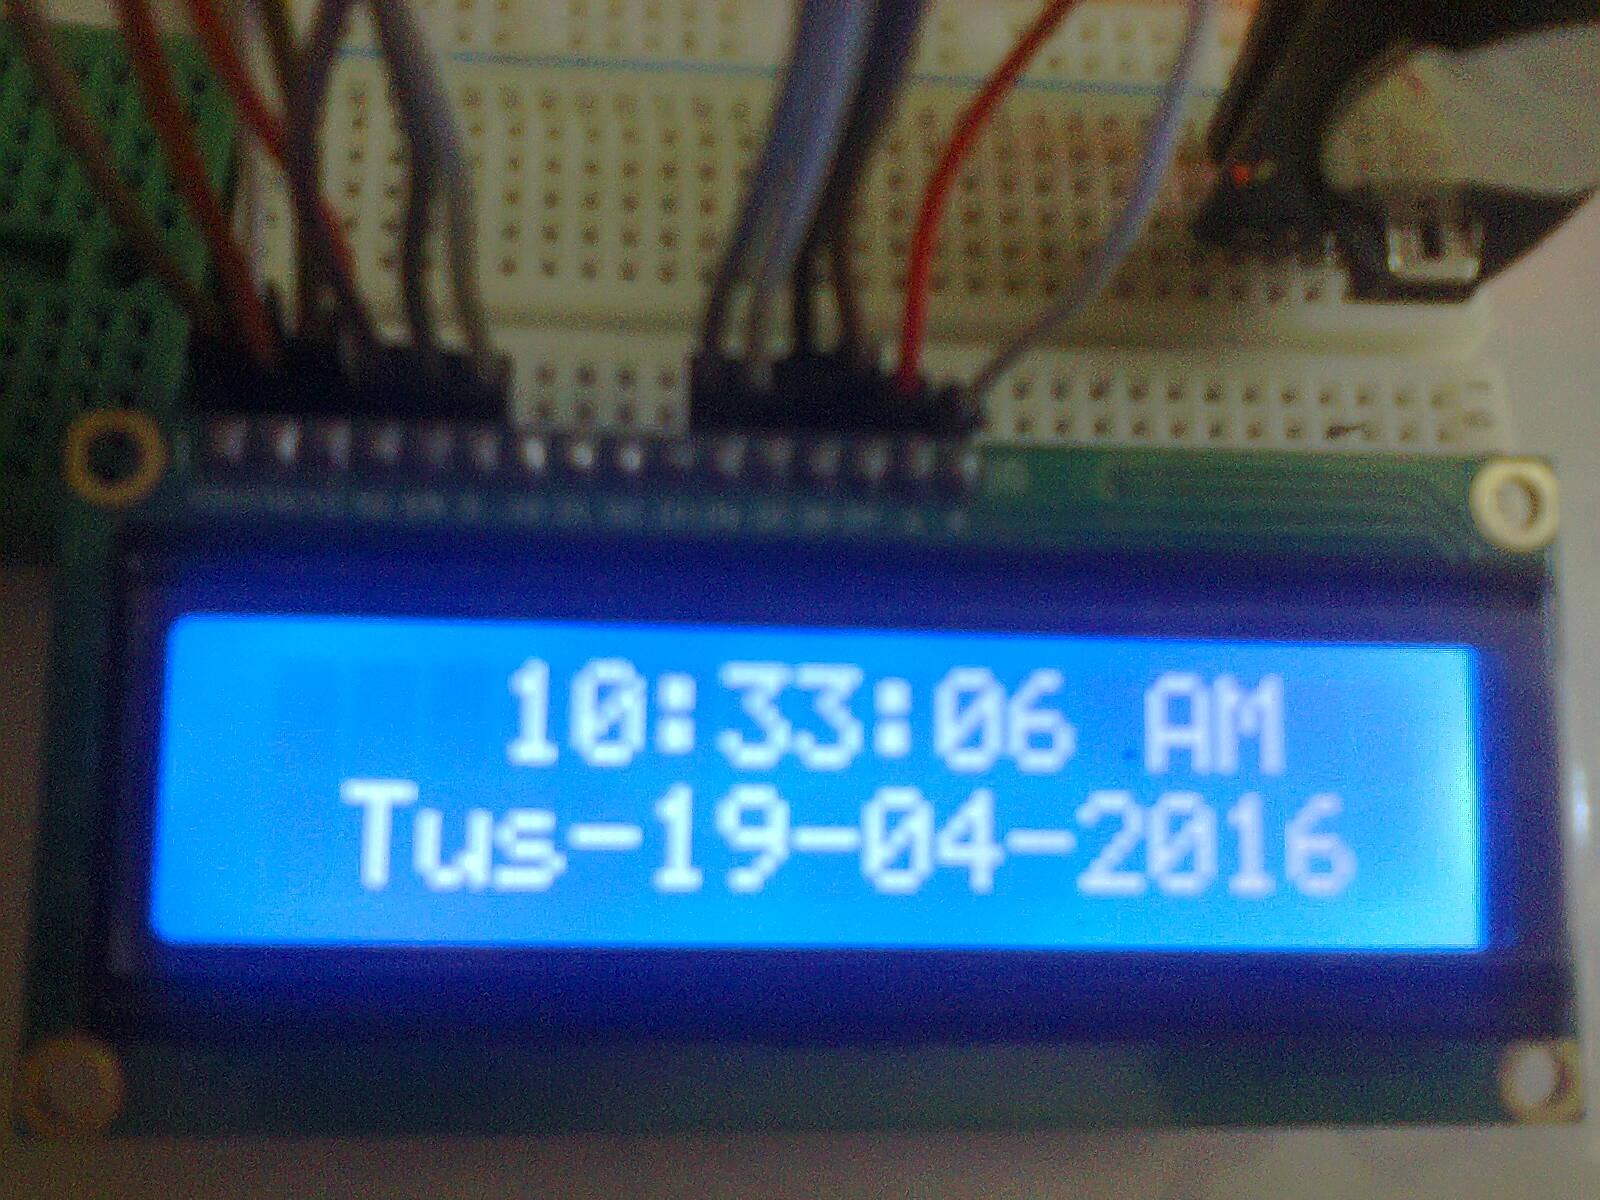
\includegraphics[width=.3\linewidth]{bai-6/image/6-2-3}}
\end{center}
\caption{Kết quả đọc thời gian thực từ IC DS3231}
\end{figure}
\subsection*{Chương trình 18 -- 1: Cài thời gian thực vào IC}
\lstinputlisting[language=C]{BAI-6-2-1.C}
\subsection*{Chương trình 18 -- 2: Lấy thời gian thực từ IC ra}
\lstinputlisting[language=C]{BAI-6-2-2.C}
\newpage
\subsection{Bài tập 6.3}
\label{Ex:ds3231-2}
\paragraph{Yêu cầu}Viết chương trình đồng hồ số hiển thị trên LCD 16x02 bao gồm giờ, phút, giây và nhiệt độ môi trường.
\paragraph{Hướng giải quyết}
\begin{itemize}
\item[$\ast$] Do sử dụng phần cứng là module RTC DS3231 nên ngoài chức năng lưu thời gian thực nó còn chức năng đọc nhiệt độ môi trường.
\item Địa chỉ của thanh ghi nhiệt độ là:
\begin{table}[!h]
\begin{center}
\begin{tabular}{|l|c|c|l|}\hline
\textit{Thanh ghi} & \textit{Địa chỉ} & \textit{Hàm} & \textit{Mô tả}\\ \hline
\verb|tempMSBREG| & \verb|0x11| & \verb|getTemp()| & Đọc vào nhiệt độ môi trường \\ \hline
\verb|tempLSBREG| & \verb|0x12| & & \\ \hline
\end{tabular}
\end{center}
\caption{IC DS3231 với chức năng đọc nhiệt độ môi trường}
\end{table}
\item Với phần thời gian thì chương trình giống như \textit{chương trình 18 -- 1} và \textit{chương trình 18 -- 2} của \textit{bài tập 6.2}. Phần nhiệt độ thì chúng ta thêm dòng lệnh sau vào vòng lặp \verb|while| và cho hiển thị giá trị đọc được lên LCD: \verb|getTemp();|
\end{itemize}
\paragraph{Sơ đồ mạch}Cách kết nối giống như \textit{bài tập 6.2}
\section*{Kết quả}
\begin{figure}[!h]
\begin{center}
%\subfloat[Sơ đồ mạch]
  {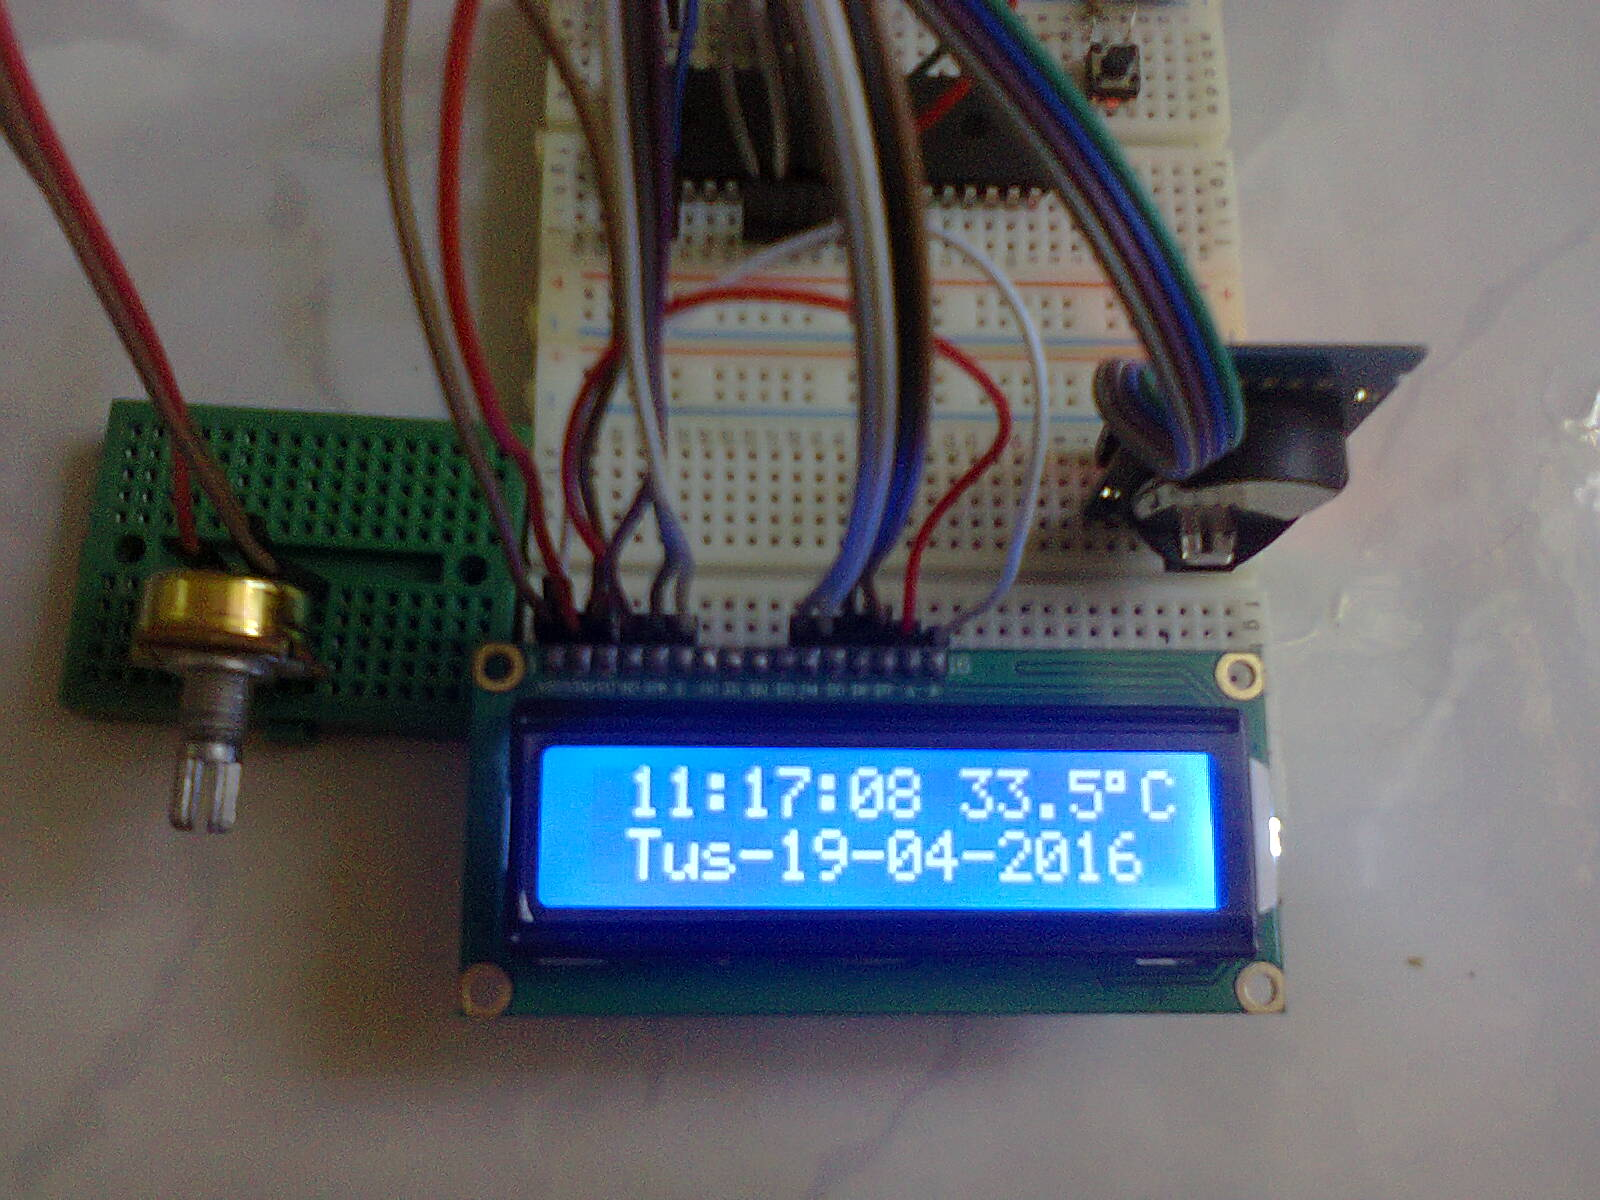
\includegraphics[width=.3\linewidth]{bai-6/image/6-3-1}}
%\subfloat[Kết quả]
  {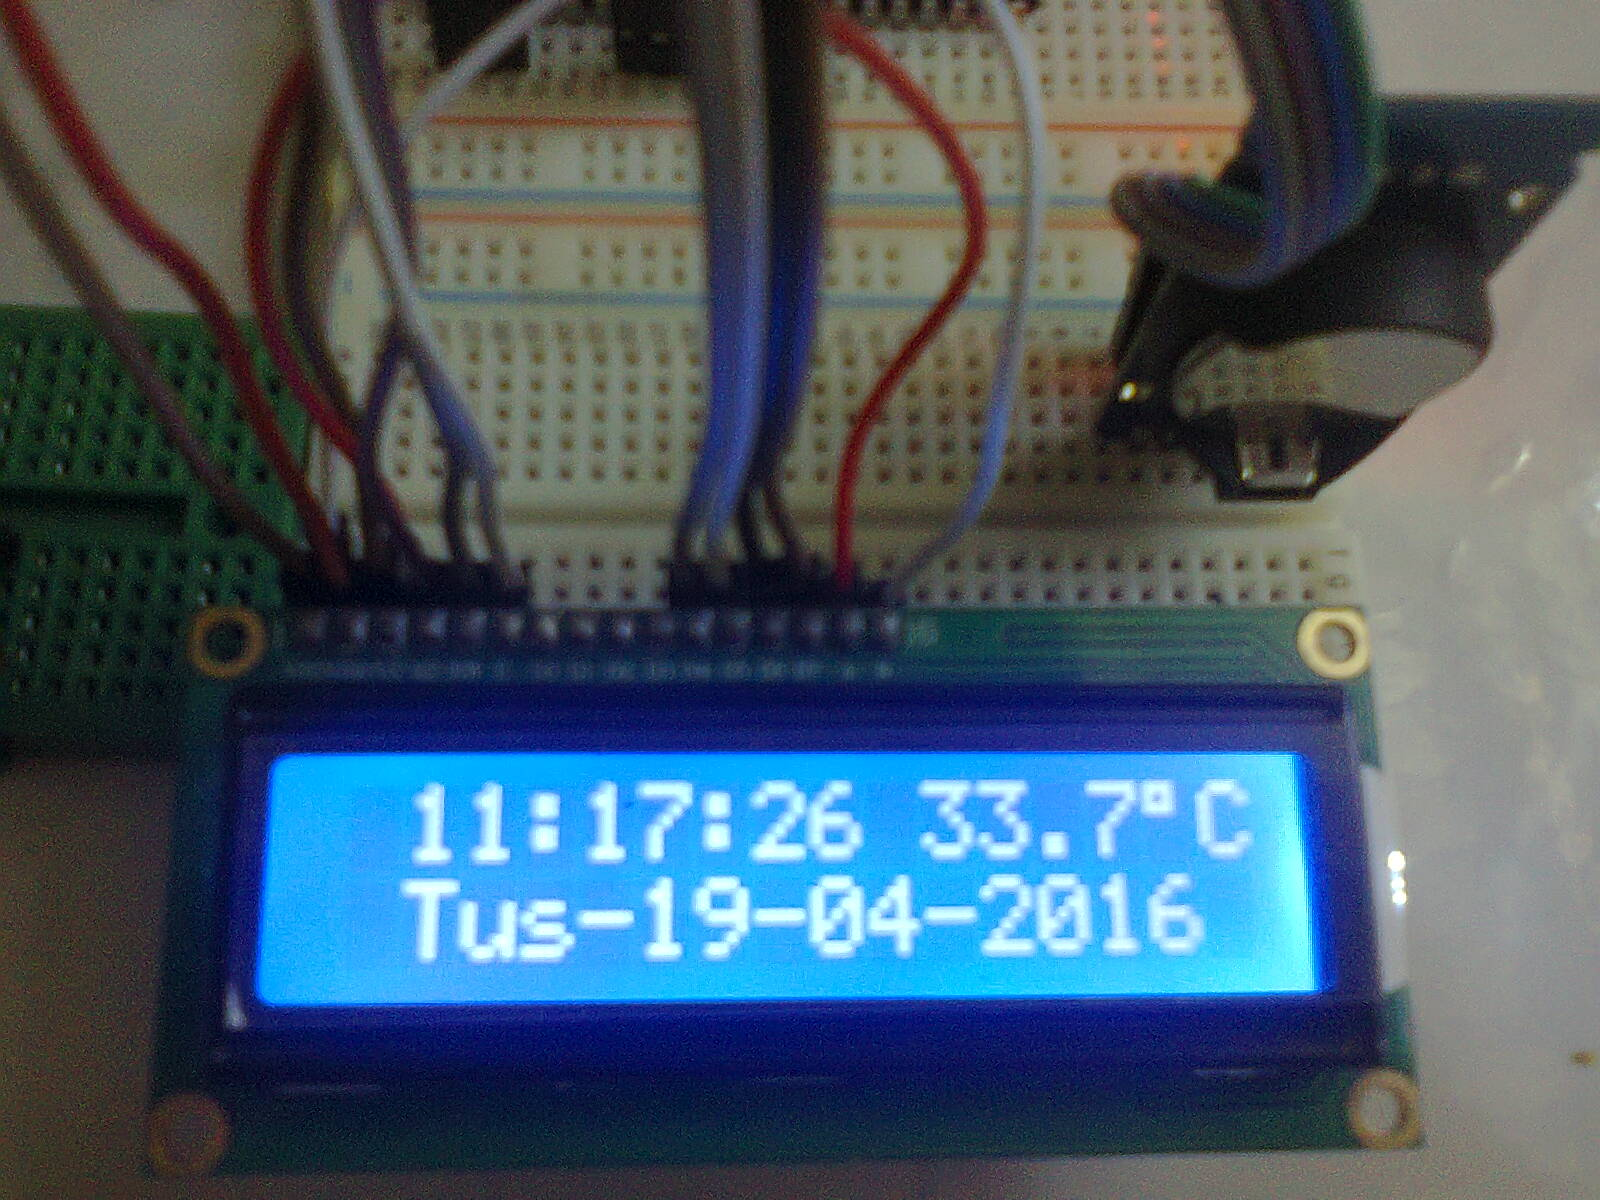
\includegraphics[width=.3\linewidth]{bai-6/image/6-3-2}}
  {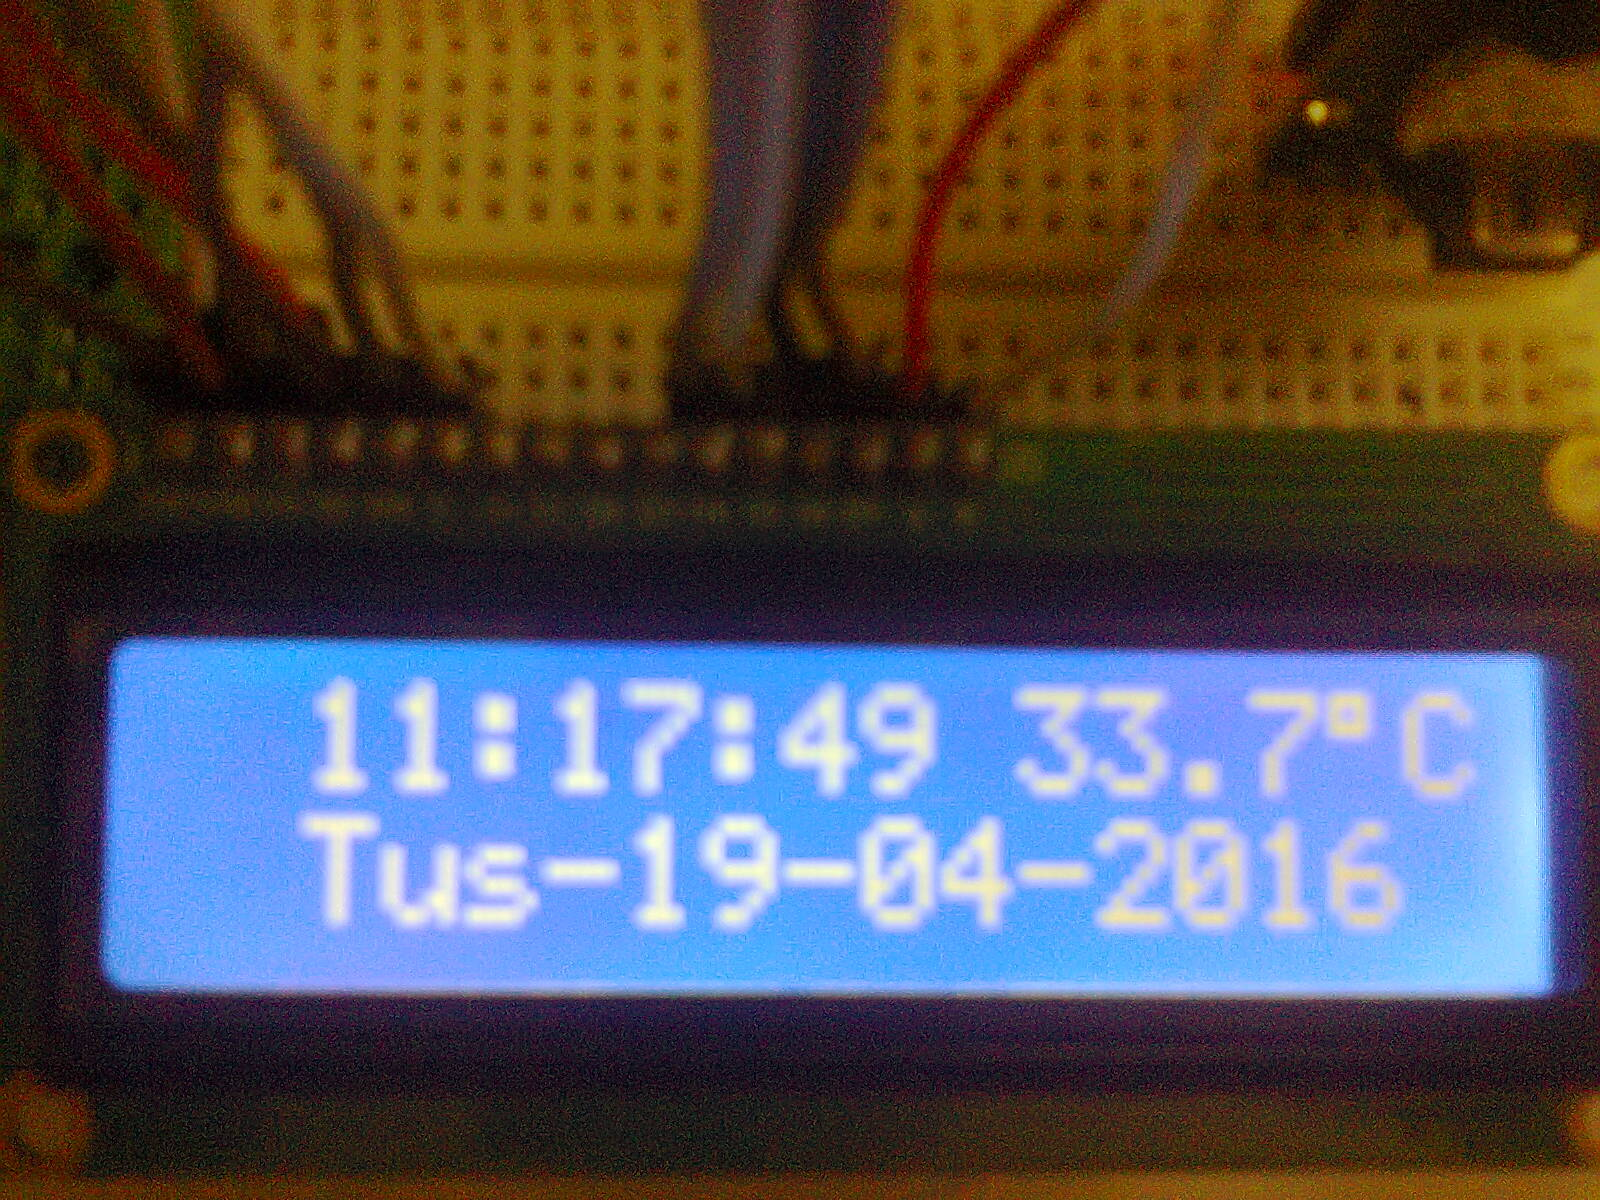
\includegraphics[width=.3\linewidth]{bai-6/image/6-3-3}}
\end{center}
\caption{Kết quả đọc thời gian thực  và nhiệt độ từ IC DS3231}
\end{figure}
\subsection*{Chương trình 19}
\label{code-19}
\lstinputlisting[language=C]{BAI-6-3.C}
\subsection{Mô phỏng cảm biến nhiệt TC74 với Protues}\label{def:TC74}
Trong quá trình tìm hiểu, em thấy có nhiều bạn gặp vấn đề khi mô phỏng cảm biến nhiệt độ TC74 với phần mềm protues. Em kiểm thử và tìm ra được là cảm biến nhiệt \verb|TC74| trong phần mềm mô phỏng \verb|Protues 7.8| nó tương thích với địa chỉ \verb|I2C| là \verb|0x9A| (đa phần các bạn làm trên địa chỉ \verb|0x90| nên khi mô phỏng thì ra giá trị nhiệt độ không đúng như đã cài đặt).

Về sơ đồ mạch và cách giải thích chương trình tương tự \textit{bài tập 6.1 trang \pageref{Ex:6-1}}.
\newpage
\paragraph{Chương trình sau mô phỏng được với phần mềm Protues 7.8}{~\\}
\lstinputlisting[language=C]{BAI-6-1V2.C}
\chapter{GIAO TIẾP RS232}
\label{chapter:rs232}
\section{Giới thiệu chung}
\subsection{Yêu cầu}
Giao tiếp giữu máy tính và vi điều khiển PIC 16F887 thông qua module RS232.
\subsection{Module RS232}
Cổng nối tiếp RS232 được sử dụng để kết nối các thiết bị ngoại vi với máy tính.

Ưu điểm: Khả năng chống nhiễu cao, tháo rời ra khỏi máy tính dễ dàng, cổng nối tiếp còn là nguồn cấp cho vi điều khiển,\ldots

Cách kết nối: Ta sử dụng 2 chân \verb|RX| và \verb|TX| của module kết nối lần lượt với 2 chân \verb|RX| và \verb|TX| của vi điều khiển (kết nối nối tiếp \verb|RX - RX| và \verb|TX - TX|).
\section{Các lệnh giao tiếp RS232}
Ta sử dụng khai báo và các lệnh sau để giao tiếp với RS232 qua cổng nối tiếp:
\begin{itemize}
\item Khai báo:
\begin{itemize}
\item Khai báo tần số thạch anh: \verb|#use delay(clock = 20000000)|, ví dụ tần số là $20MHz$
\item Khai báo RS232: 

\verb|#use RS232(BAUD = 9600, PARITY = N, XMIT = PIN_C6, RCV = PIN_C7)|

với \verb|BAUD = 9600|: tốc độ truyền; \verb|PARITY = N|: không kiểm tra chẳn lẻ; \verb|XMIT = PIN_C6|: chân truyền là \verb|C6|; \verb|RCV = PIN_C7|: chân nhận là \verb|C7|.
\end{itemize}
\item Các lệnh giao tiếp: \verb|printf|, \verb|getc|, \verb|getch|, \verb|getchar|, \verb|fgetc|, \verb|gets|, \verb|fgets|, \verb|puc|, \verb|putchar|, \verb|fputc|, \verb|puts|, \verb|fputs|, \verb|kbhit|, \verb|assert|, \verb|perror|, \verb|set_uart_speed|, \verb|setup_uart|.
\end{itemize}
\section{Bài tập}
\subsection{Bài tập 7.1}
\paragraph{Yêu cầu}Viết chương trình truyền dữ liệu giữa PC và PIC 16F887 với yêu cầu sau:
Truyền ký tự \verb|'b'| và \verb|'t'| từ PC thông qua chương trình MATLAB, khi PIC nhận được ký tự \verb|'b'| thì bật các LED ở PORT E, khi nhận được ký tự \verb|'t'| thì tắt các LED ở PORT E.
\paragraph{Hướng giải quyết}
\begin{itemize}
\item Chúng ta thực hiện truyền dữ liệu qua cổng nối tiếp RS232 để thực hiện giao tiếp giữa PC và PIC.
\item Khai báo RS232: chọn tốc độ truyền là \verb|9600|

\verb|#use RS232(BAUD = 9600, PARITY = N, XMIT = PIN_C6, RCV = PIN_C7)|
\item Sử dụng ngắt nhận dữ liệu từ RS232 là \verb|#INT_RDA|.
\begin{itemize}
\item Khai báo ngắt: 

\verb|ENABLE_INTERRUPTS(INT_RDA);| và \verb|ENABLE_INTERRUPTS(GLOBAL);|
\item Chương trình ngắt: 
\begin{itemize}
\item Nội dung chương trình ngắt:
\begin{itemize}
\item[+] Đọc giá trị từ PC gửi qua PIC: \verb|value = getc();|
\item[+] Nếu \verb|value = 'b'| thì đưa PORT E lên mức cao: \verb|PORTE = 0xFF;|
\item[+] Nếu \verb|value = 't'| thì đưa PORT E lên mức thấp: \verb|PORTE  0x00;|
\end{itemize}
\end{itemize}
\end{itemize}
\item Khai báo PORT E là OUTPUT: \verb|TRISE = 0x00;|
\item Sử dụng phần mềm MATLAB để gửi dữ liệu đến PIC:
\begin{itemize}
\item Xác định  tên cổng nối tiếp , ta dùng \verb|s = serial(tên_port,tốc_độ_truyền)| với Windows thì \verb|tên_port = 'com1'| (còn những hệ điều hành khác, chúng ta có thể xem hướng dẫn về \verb|serial| trong phần \verb|Help| của MATLAB); \verb|tốc_độ_truyền| bằng tốc độ truyền ta khai báo trong chương trình CCS. 
\item Mở port dùng: \verb|fopen(s)|.
\item Gửi giá trị qua port dùng: \verb|fprintf(s,'giá_trị_gửi')|.

Ví dụ: \verb|fprintf(s,'b')|.
\item Nếu không gửi dữ liệu tiếp, ta thực hiện đóng port dùng: \verb|fclose(s)|.
\end{itemize}
\end{itemize}
\newpage
\subsection*{Sơ đồ mạch}
\begin{figure}[!h]
\begin{center}
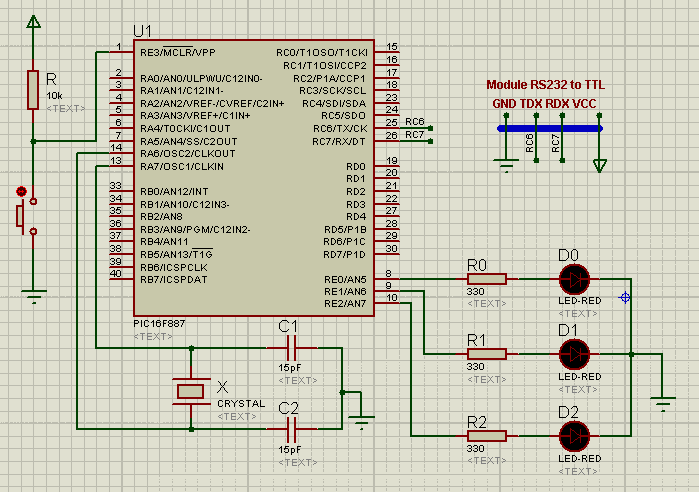
\includegraphics[scale=0.6]{bai-7/image/BAI-7-1}
\end{center}
\caption{Mạch sử dụng module RS232 to TTL nhận lệnh từ PC bật tắt LED ở PORT E}
\end{figure}
\subsection*{Chương trình 20}
\lstinputlisting[language=C]{BAI-7-1.C}

Chương trình nhận lệnh điều khiển từ PC với code Matlab (thực hiện lần lượt các lệnh sau bằng \verb|Command line|):
\lstinputlisting[language=Matlab]{BAI-7-1.m}
\subsection{Bài tập 7.2}
\paragraph{Yêu cầu}Viết chương trình truyền chuỗi \verb|"TT VI DIEU KHIEN"| từ PC xuống máy tính và hiển thị chuỗi nhận được lên LCD 16x02.
\paragraph{Hướng giải quyết}
\begin{itemize}
\item[$\ast$] Chúng ta dựa vào \textit{chương trình 20}, nhưng thay đổi một số chỗ cho phù hợp.
\item \textit{Chương trình ngắt}: Để đọc được một chuỗi từ PC truyền xuống, dùng hàm \verb|gets(string)| thay cho hàm \verb|getc()| (chỉ đọc được 1 ký tự).
\item \textit{Chương trình chính}: ta thêm các lệnh khởi tạo LCD (thêm vào thư viện \verb|LCD_LIB4BIT.C| ở phần khai báo đầu). Trong vòng lặp \verb|while| cho hiển thị chuỗi \verb|"TT VI DIEU KHIEN"| nhận được từ PC lên LCD.
\item[$\ast$] Khi chạy thực tế, đôi khi phần cứng bị nhiễu, đã nhận được chuỗi ký tự nhưng mà chưa hiển thị lên LCD thì nhấn nút Reset là chuỗi được hiển thị lên LCD.
\end{itemize}
\newpage
\subsection*{Sơ đồ mạch}
\begin{figure}[!h]
\begin{center}
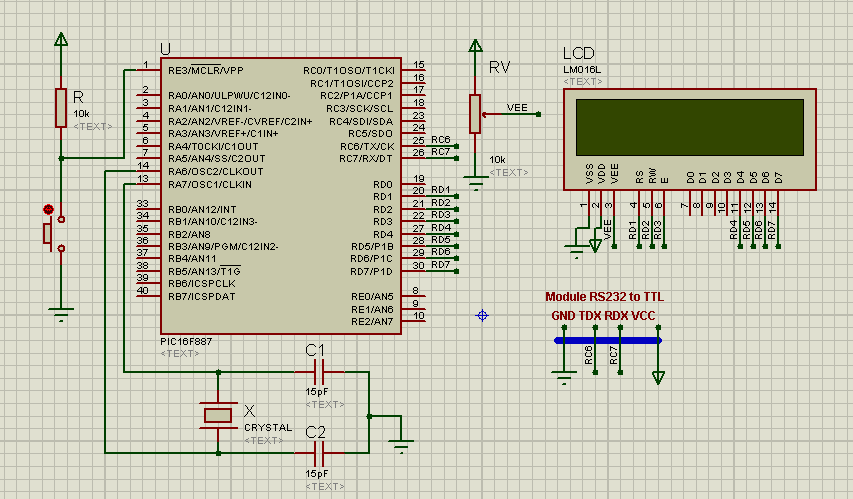
\includegraphics[scale=0.6]{bai-7/image/BAI-7-2}
\end{center}
\caption{Mạch sử dụng module RS232 to TTL nhận chuỗi từ PC hiển thị lên LCD}
\end{figure}
\subsection*{Chương trình 21}
\lstinputlisting[language=C]{BAI-7-2.C}

Chương trình nhận lệnh điều khiển từ PC với code Matlab (thực hiện lần lượt các lệnh sau bằng \verb|Command line|):
\lstinputlisting[language=Matlab]{BAI-7-2.m}
\subsection{Bài tập 7.3}
\paragraph{Yêu cầu}Viết chương trình đọc giá trị nhiệt độ từ IC TC74 sau đó truyền giá trị đọc được lên PC qua cổng RS232.
\paragraph{Hướng giải quyết}
\begin{itemize}
\item Do không có IC TC74, nên em thay thế bằng phần cứng khác là IC DS3231 (trong \textit{bài tập 6.2} và \textit{bài tập 6.3} \textit{trang \pageref{Ex:ds3231-1}} và \textit{trang \pageref{Ex:ds3231-2}}), nó có chức năng lưu thời gian thực và đọc nhiệt độ môi trường. 
\item Sự dụng IC với chức năng đọc nhiệt độ (trong \textit{bài tập 6.3 trang \pageref{Ex:ds3231-2}}) nên chúng ta rút ngắn lại \textit{chương trình 19 trang \pageref{code-19}}.
\item Sau khi đọc được nhiệt độ dùng lệnh \verb|printf("%.1fC", getTemp());| để gửi lên máy tính.
\item Sử dụng LCD để kiểm chứng lại kết quả gửi lên máy tính.
\item Phần code Matlab hoàn toàn giống \textit{bài tập 4.3 trang \pageref{Ex:4-3}}.
\end{itemize}
\newpage
\subsection*{Sơ đồ mạch}
\begin{figure}[!h]
\begin{center}
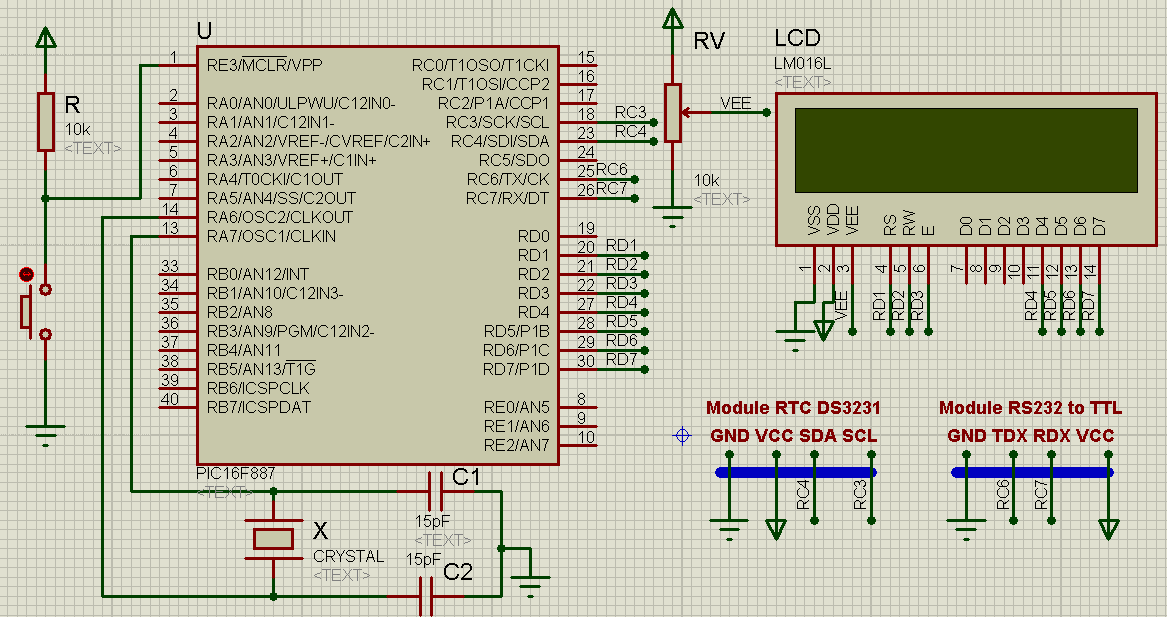
\includegraphics[scale=0.5]{bai-7/image/BAI-7-3}
\end{center}
\caption{Mạch sử dụng module RS232 to TTL gửi nhiệt độ từ IC DS3231 lên PC}
\end{figure}
\subsection*{Chương trình 22}
\lstinputlisting[language=C]{BAI-7-3.C}

Hàm \verb|Serial_Callback| dùng để thiết lập cho tham số \verb|BytesAvailableFcn| trước khi mở cổng COM:
\lstinputlisting[language=Matlab]{Serial_Callback.m}

Lệnh Matlab nhận dữ liệu từ vi điều khiển gửi lên:
\lstinputlisting[language=Matlab]{BAI-7-3.m}
\chapter{ĐIỀU KHIỂN ĐỘNG CƠ DC}
\section{Giới thiệu chung}
\subsection{Yêu cầu}Điều khiển chiều quay và tốc độ động cơ DC.
\subsection{Động cơ DC}
Để động cơ hoạt động được, ta cấp điện áp vào động cơ, xuất hiện dòng điện chạy các cuộn dây trong động cơ, làm động cơ quay theo một chiều xác định, để đổi chiều quay ta đổi chiều điện áp. Khi điều khiển động cơ: không được cấp điện áp và dòng điện quá giá trị định mức ghi trên động cơ (cấp thấp hơn động cơ vẫn hoạt động được).
\section{Các bài toán điều khiển động cơ}
\subsection{Điều khiển chiều quay của động cơ}
Để điều khiển chiều quay của động cơ, người ta sử dụng mạch cầu H để làm điều này.

\begin{figure}[!h]
\begin{center}
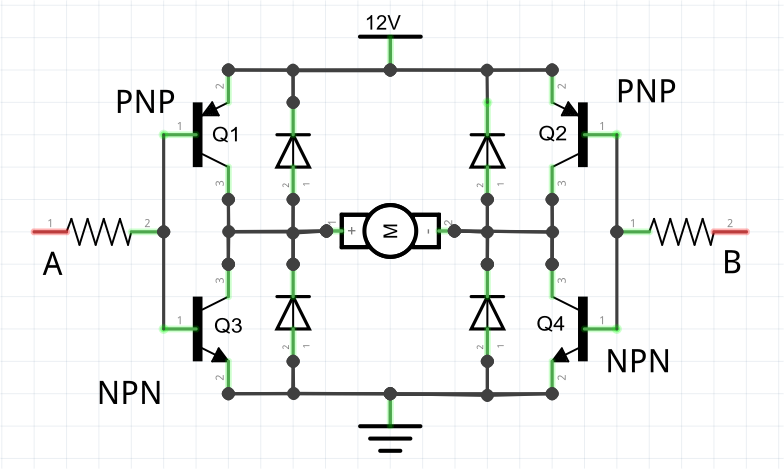
\includegraphics[scale=0.3]{bai-8/image/mach-cau-H}
\end{center}
\caption{Mạch cầu H điều khiển chiều quay của động cơ}
\end{figure}
\newpage
Chọn IC L293D để thực hiện chức năng của mạch cầu H điều khiển chiều quay của động cơ. Cụ thể như sau:
\begin{figure}[!h]
\begin{center}
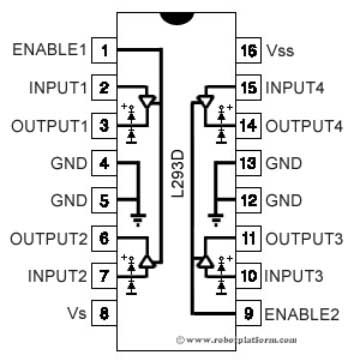
\includegraphics[scale=0.35]{bai-8/image/L293D}
\end{center}
\caption{Sơ đồ chân IC L293D}
\end{figure}
\begin{itemize}
\item Số chân của IC: 16 chân (6 chân điều khiển tín hiệu; 4 chân điều khiển động cơ; 2 chân cấp nguồn; 4 chân đất), IC điều khiển được 2 động cơ.
\item Các chân điều khiển: \verb|ENABLE1|, \verb|INPUT1|, \verb|INPUT2| (động cơ 1) và \verb|ENABLE2|, \verb|INPUT3|, \verb|INPUT4| (động cơ 2). Cụ thể chiều quay được xác định như sau:
\begin{itemize}
\item[$\ast$] Ta xác định cách điều khiển cho động cơ thứ nhất.
\item Chiều ngược chiều kim đồng hồ: \verb|ENABLE1 = 1|, \verb|INPUT1 = 1|, \verb|INPUT2 = 0|.
\item Chiều cùng chiều kim đồng hồ: \verb|ENABLE1 = 1|, \verb|INPUT1 = 0|, \verb|INPUT2 = 1|.
\item Dừng động cơ khi \verb|ENABLE1 = 0| (bất kể \verb|INPUT1| và \verb|INPUT2| ở mức cao hay mức thấp).
\item[$\ast$] Động cơ thứ 2 cũng thực hiện tương tự như vậy: ta dùng các chân \verb|ENABLE2|, \verb|INPUT3|, \verb|INPUT4|.
\end{itemize}
\item Cấp nguồn: chân \verb|VSS| lấy nguồn của vi điều khiển, chân \verb|Vs| lấy nguồn ngoài cấp cho động cơ (không nên dùng chung nguồn với vi điều khiển).
\item Chân nối động cơ: \verb|OUTPUT1|, \verb|OUTPUT2| cho động cơ 1; \verb|OUTPUT3|, \verb|OUTPUT4| cho động cơ 2.
\end{itemize}
\subsection{Điều khiển tốc độ quay của động cơ}
Ta sử dụng phương pháp điều chế độ rộng xung -- \verb|PWM| để điểu khiển tốc độ động cơ. Ví dụ như trong các giản đồ xung \textit{hình \ref{pwm}}:
\begin{figure}[!h]
\begin{center}
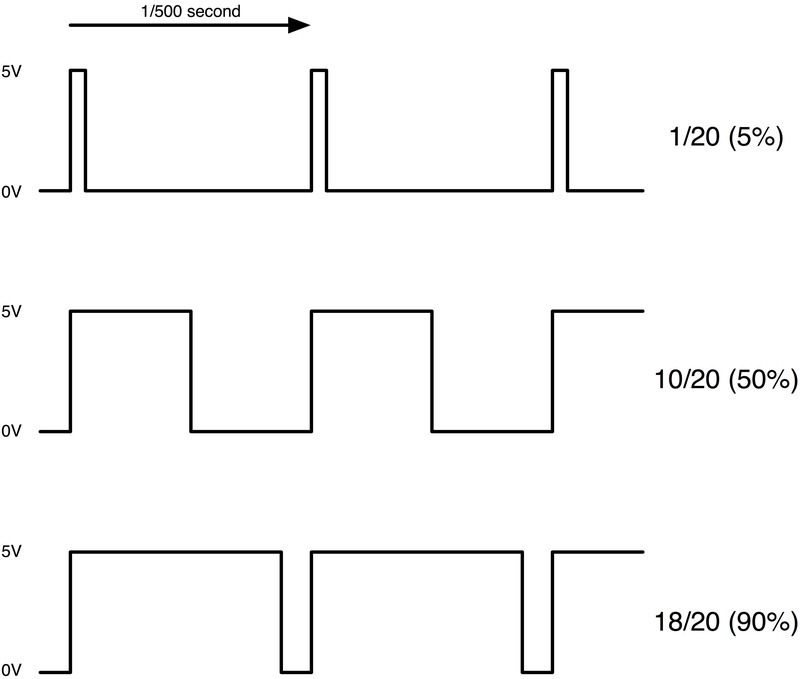
\includegraphics[width=.3\linewidth]{bai-8/image/pwm-1}
\end{center}
\caption{Phương pháp điều chế độ rộng xung} \label{pwm}
\end{figure}

Khối \verb|PWM| trên PIC 16F887 có 2 mạch so sánh: \verb|8 bit| (so sánh với giá trị đếm của \verb|timer2|) và \verb|10 bit|.\\

Ta thực hiện điều chế độ rộng xung bằng phần cứng (dùng chân \verb|CCP1| hoặc \verb|CCP2|). Tiến hành tính toán và thiết lặp các giá trị sau:
\begin{itemize}
\item Xác định tần số điều xung \verb|PWM| qua khai báo sau:

\verb|setup_timer_2(mode, period, postscale);|

suy ra: $\displaystyle f = \frac{f_{osc}}{4 \times mode \times \left({period+1}\right)}$ với:
\begin{itemize}
\item \verb|mode|: \verb|T2_DIV_BY_1|, \verb|T2_DIV_BY_4|, \verb|T2_DIV_BY_16|.
\item \verb|period|: $0-255$.
\item \verb|postscale|: $1$.
\end{itemize}
\item Kích hoạt chế độ \verb|PWM|: \verb|setup_ccp1(cpp_pwm)| hoặc \verb|setup_ccp2(cpp_pwm)|.
\item Xác định hệ số chu kỳ xung thông qua khai báo:


\verb|set_pwm1_duty(value)| hoặc \verb|set_pwm2_duty(value)|
\begin{itemize}
\item Nếu \verb|value| là số nguyên 8 bit: $\displaystyle duty cycle = \frac{value}{period + 1}$.
\item Nếu \verb|value| là số nguyên 16 bit: $\displaystyle duty cycle = \frac{value \times 1023}{4 \times \left({period + 1}\right)}$.
\end{itemize}
\item[$\ast$] Nếu ứng dụng không cần điều chế xung mịn thì ta có thể dùng \textit{8 bit}.
\end{itemize}
\section{Bài tập}
\subsection{Bài tập 8.1}
\paragraph{Yêu cầu}Viết chương trình điều khiển chiều quay động cơ bằng nút nhấn nối với ngắt ngoài của vi điều khiển PIC 16F887.
\paragraph{Hướng giải quyết}
\begin{itemize}
\item Ta sử dụng ngắt ngoài \verb|#INT_EXT| (ngắt trên chân B0) để điều khiển chiều quay của động cơ thông qua số lần nhấn nút \verb|count|:
\item Khi chưa nhấn nút nhấn (\verb|count = 0|): động cơ chưa quay.
\item Khi nhấn nút lần đầu tiên (\verb|count%2 = 1|): động cơ quay theo chiều thuận: \verb|ENABLE1 = 1|, \verb|INPUT1 = 1|, \verb|INPUT2 = 0|.
\item Khi nhấn nút lần thứ 2 (\verb|count%2 = 0|): động cơ quay theo chiều nghịch: \verb|ENABLE1 = 1|, \verb|INPUT1 = 0|, \verb|INPUT2 = 1|.
\item Lặp lại quá trình trên.
\item \textit{Lưu ý}: tùy vào phần cứng của chúng ta có bị nhiễu hay không mà ta có thể khai báo giá trị ban đầu của biến \verb|count| là: \verb|count = 0| hay \verb|count = -1|.
\end{itemize}
\newpage
\subsection*{Sơ đồ mạch}
\begin{figure}[!h]
\begin{center}
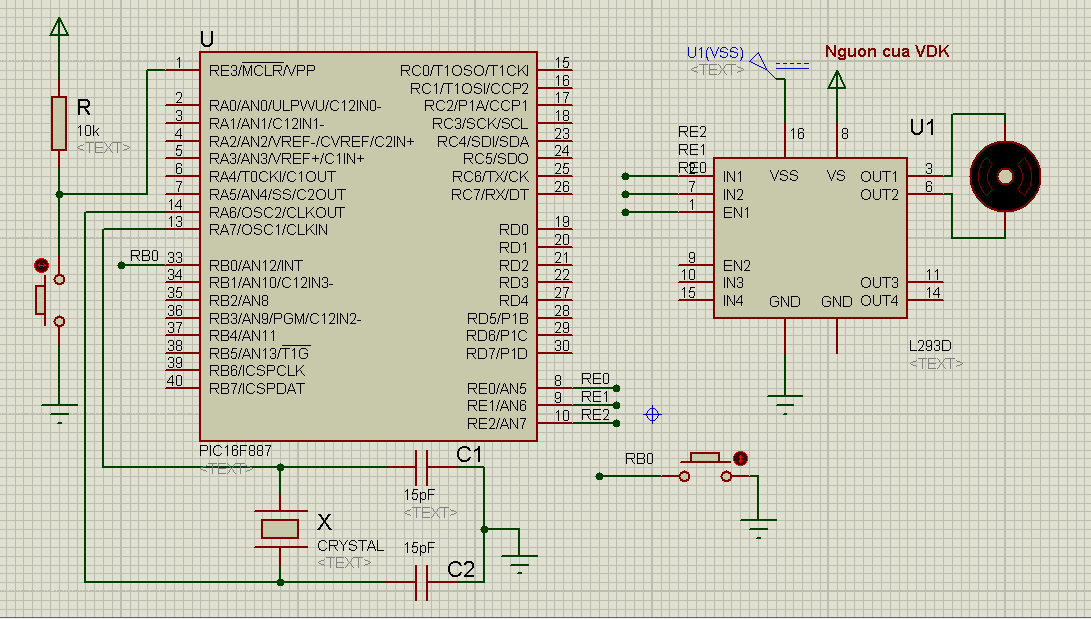
\includegraphics[scale=0.5]{bai-8/image/BAI-8-1}
\end{center}
\caption{Mạch đảo chiều động cơ với IC L293D}
\label{Fig:dao-chieu}
\end{figure}
\subsection*{Chương trình 23}
\lstinputlisting[language=C]{BAI-8-1.C}
\subsection{Bài tập 8.2}
\paragraph{Yêu cầu}Viết chương trình điều khiển tốc độ và chiều quay của động cơ.
\paragraph{Hướng giải quyết}
\begin{itemize}
\item Do đề bài không đưa ra yêu cầu cụ thể là điều khiển như thế nào, nên ta đặt ra yêu cầu cụ như sau:
\begin{itemize}
\item Khi chưa nhấn nút nhấn trạng thái 0: động cơ không quay.
\item Khi nhấn nút nhấn lần đầu tiên -- trạng thái 1: động cơ quay theo chiều của kim đồng hồ (quay thuận) và tốc độ tăng dần sau mỗi $1s$, đến khi ổn định tốc độ thì giảm dần tốc độ sau mỗi $1s$.
\item Nhấn nút nhấn lần thứ 2 -- trạng thái 2: động cơ quay ngược chiều của chiều kim đồng hồ (quay nghịch) và tốc độ tăng dần sau mỗi $1s$, đến khi ổn định tốc độ thì giảm dần tốc độ sau mỗi $1s$.
\end{itemize}
\item Ví dụ, ta cần điều chế một xung có tần số điều xung là $f = 10kHz$ thì ta cần chọn: $\displaystyle mode \times \left({period + 1}\right) = \frac{f_{osc}}{4 \times f} = \frac{20 \times 10^6}{4 \times 10 \times 10^3} = 500$, ta có bảng:
\begin{center}
\begin{tabular}{c|c}
\textit{mode} & \textit{period}\\ \hline
$1$ & $499$\\
$4$ & $124$\\
$16$ & $30.25$\\
\end{tabular}
\end{center}
Chọn cách khai báo sau: \verb|setup_timer_2(T2_DIV_BY_4,124,1);| sẽ tạo ra được một xung có tần số là $10kHz$.
\item Tăng hoặc giảm tốc độ, ta cần tăng hoặc giảm giá trị của tham số \verb|value| trong hàm \verb|set_pwm1_duty(value)|.

Ta giả sử \verb|set_pwm1_duty(dutycycle) = 100%|, thì xem \verb|value| có giá trị là bao nhiêu:
\begin{align*}
value & = \frac{1}{f} \times dutycycle \times \frac{f_{osc}}{mode} \\
& = \frac{1}{10kHz} \times 100\% \times \frac{20MHz}{4} \\
& = \frac{1}{10\times 10^3} \times 1 \times \frac{20 \times 10^6}{4} = 500
\end{align*}
\item Thực hiện vòng lặp \verb|for| tăng dần giá trị của \verb|value| nhưng phải luôn kiểm tra điều kiện $value \leq 500$.
\item Phần trên ta chỉ điều khiển được tốc độ, tiếp theo ta sẽ điều khiển chiều quay của động cơ: sử dụng IC L293D với chân \verb|ENABLE1| nối tắt lên nguồn, còn 2 chân \verb|INPUT1| và \verb|INPUT2| ta nối với 2 chân \verb|CCP1| và \verb|CCP2| để điều chế độ rộng xung cấp cho động cơ, việc đảo chiều tương tự như \textit{bài tập 8.1 trong chương trình 23}.
\item Cấu hình các chân điều khiển: \verb|PORTB = 0xFF| (chân \verb|INPUT|) và \verb|PORTC = 0x00| (chân \verb|OUTPUT|). Ta vẫn sử dụng ngắt ngoài ở B0 để dùng lại \textit{chương trình 23}.
\end{itemize}
%\subsection*{Sơ đồ mạch}
\paragraph{Sơ đồ mạch} giống sơ đồ \textit{bài tập 8.1} \textit{hình \ref{Fig:dao-chieu}} \textit{trang \pageref{Fig:dao-chieu}}.
\begin{comment}
\begin{figure}[!h]
\begin{center}
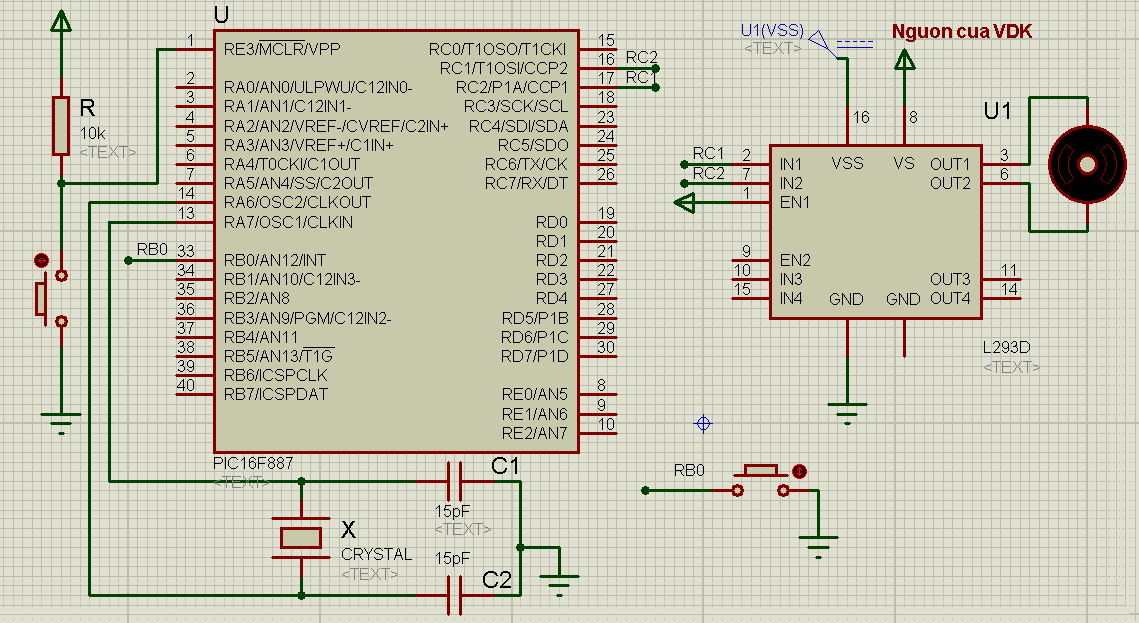
\includegraphics[scale=0.5]{bai-8/image/BAI-8-2}
\end{center}
\caption{Mạch đảo chiều động cơ và điều khiển tốc độ với IC L293D}
\end{figure}
\end{comment}
\subsection*{Chương trình 24}
\lstinputlisting[language=C]{BAI-8-2.C}
%\subsection{Bài tập 8.3}
%\paragraph{Yêu cầu}Viết chương trình đo tốc độ động cơ DC và hiển thị lên LCD 16x02.
%\subsection*{Chương trình 25}
%\subsection{Bài tập 8.4}
%\paragraph{Yêu cầu}Viết chương trình điều khiển tốc độ động cơ DC bằng PC qua cổng RS232.
%\paragraph{Hướng giải quyết}
%\begin{itemize}
%\item[$\ast$] Ta dự theo \textit{chương trình 24} của \textit{bài tập 8.2} với một số thay đổi phù hợp.
%\end{itemize}
%\subsection*{Chương trình 26}
\subsection{Điều khiển tốc độ động cơ với Transistor}
\paragraph{Sơ đồ mạch}{~\\}
\begin{figure}[!h]
\begin{center}
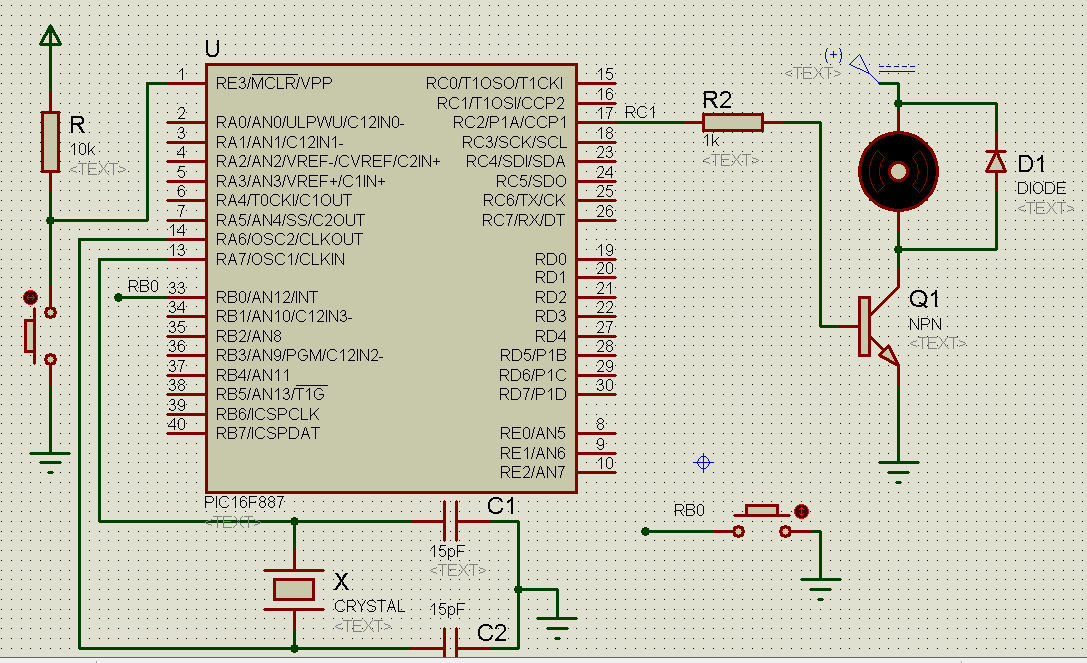
\includegraphics[scale=.5]{bai-8/image/BAI-8-2-2}
\end{center}
\caption{Điều khiển tốc độ động cơ với Transistor}
\end{figure}\\

Nội dung của chương trình: 
\subsection*{Chương trình 25}
\lstinputlisting[language=C]{BAI-8-2-1.C}
\chapter{ĐO KHOẢNG CÁCH BẰNG CẢM BIẾN SIÊU ÂM SRF05}
\section{Giới thiệu chung}
\subsection{Yêu cầu}
Sử dụng vi điều khiển PIC 16F887 lập trình đo khoảng cách với cảm biến siêu âm SRF05.
\subsection{Cảm biến siêu âm SRF05}
Nguyên lý đo khoảng cách của cảm biến siêm âm SRF05:
\begin{itemize}
\item Dùng nguyên lý phản xạ sóng để đo vật cản.
\item Cảm biến phát đi một lúc 8 xung với tần số $40kHz$, gặp vật cản xung phát đi sẽ dội về. Từ đây, có thể tính được khoảng cách.
\item Khi phát xung đi, chân Echo ở mức cao, nhận xung dội về, chân Echo xuống mức thấp (hoặc sau $30ms$ không nhận được cũng xuống mức thấp).
\end{itemize}

Cảm biến có 2 chế độ hoạt động: chân Trigger và chân Echo dùng riêng hoặc dùng chung.
\begin{itemize}
\item Chân Trigger và chân Echo dùng riêng:
\item Chân Trigger và chân Echo dùng chung:
\end{itemize}
\section{Đo khoảng cách với cảm biến siêu âm}
Đo khoảng cách với cảm biến siêu âm chính là đo thời gian chân Echo ở mức cao. Ta thực hiện theo các bước sau:
\begin{itemize}
\item Kích chân Trigger: Xuất ra mức cao ở chân Trigger và delay tối thiểu $10\mu s$.
\item Đợi chân Echo lên mức cao.
\item Khi chân Echo lên mức cao, kích hoạt Timer: có 2 cách thực hiện:
\begin{itemize}
\item Đợi chân Echo xuống mức thấp.
\item Cho phép ngắt cạnh xuống (sử dụng với ngắt).
\end{itemize}
\item Khi chân Echo xuống mức thấp, dừng Timer, tính thời gian từ Timer rồi suy ra khoảng cách.
\begin{itemize}
\item Có $v = 344 m/s = 344 \times 10^2 \times 10^{-6} = 0.0344 cm/\mu s$. Thời gian $t$ đơn vị là $\mu s$.
\item Công thức tính khoảng cách:
\begin{align*}
S = 2 \times d \Longleftrightarrow d = \frac{S}{2} = \frac{v \times t}{2} = \frac{0.0344 \times t}{2} = \frac{t}{58.14} ~cm
\end{align*}
\item[$\ast$] Nếu sau $30ms$ mà không gặp vật cản thì chân $Echo$ cũng sẽ xuống mức thấp.
\end{itemize}
\item Reset lại giá trị của Timer để chuẩn bị cho các lần đo tiếp.
\end{itemize}
\section{Bài tập}
\subsection{Bài tập 9.1}
\paragraph{Yêu cầu}Viết chương trình đo khoảng cách bằng cảm biến siêu âm kết nối với vi điều khiển PIC 16F887.
\begin{comment}
\paragraph{Hướng giải quyết}
\begin{itemize}
\item[$\ast$] Viết chương trình theo mode 1: chân Echo và chân Trigger dùng riêng.
\item[$\ast$] Sử dụng Timer 1 kết hợp với ngắt để đếm thời gian chân Echo ở mức cao.
\item Khai báo chân chân Trigger là chân OUTPUT, chân Echo là chân INPUT nối với ngắt ngoài của vi điều khiển (chân B0).
\item Xuất mức 1 ra chân Trigger và giữ trạng thái $10\mu s$ rồi kéo chân Trigger xuống mức 0.
\item Dùng câu lệnh sau để đợi chân Echo lên mức cao: \verb|while (input(echo == 0));| không làm gì cả. Khi chân Echo lên mức cao, sẽ tự thoát khỏi vòng lặp \verb|while|.
\item Kích hoạt Timer 1 để đếm thời gian: \verb|SET_TIMER1(0);| bắt đầu đếm từ 0.
\item Đợi chân Echo xuống mức thấp: sử dụng ngắt ngoài để phát hiện xung cạnh xuống: \verb|EXT_INT_EDGE(H_TO_L);|
\item Khi phát hiện có ngắt:
\begin{itemize}
\item Kiểm tra có phải ngắt do nhiễu hay ngắt đúng mong muốn: sử dụng lại phương pháp trong \textit{bài tập \ref{Ex:3-4} trang \pageref{Ex:3-4}}.
\item Nếu không phải ngắt do nhiễu thì ta xử lý:
\begin{list}{+}{}
\item Tần số thạch anh là: $f = 20MHz$, tần số xung nội: $$ F^\prime = \frac{F}{4} = \frac{20MHz}{4} = 5MHz$$.
\item Nên sẽ thực hiện $5000$ xung trong $1ms$.
\item Giá trị tối đa của Timer 1 là $65535$, suy ra: Timer 1 đếm được tối đa là $\displaystyle \frac{65535}{5000} = 13.107ms < 30ms$, nên ta sử dụng bộ chia 4.
\item Với bộ chia 4 thì Timer 1 đếm được tối đa $4 \times 13.107 = 52.428ms > 30ms$, thỏa điều kiện.
\item[$\ast$] \textit{Kết luận}: Với bộ chia 4 -- $1ms$ thực hiện $1250$ xung, suy ra: $1\mu s$ thực hiện $1.25$ xung. Suy ra: thời gian đếm được: $$t = 1.25 \times GET\_TIMER1()$$
\item Tính ra khoảng cách: $\displaystyle d = \frac{t}{58.14} ~cm$
\item Reset lại Timer1: \verb|SET_TIMER1(0);|
\end{list}
\end{itemize}
\end{itemize}
\end{comment}
\subsection*{Chương trình 26}
\lstinputlisting[language=C]{BAI-9-1.C}
\subsection{Bài tập 9.2}
\paragraph{Yêu cầu}Viết chương trình đo khoảng cách bằng cảm biến siêu âm kết nối với vi điều khiển PIC 16F887 và gửi giá trị đo được lên máy tính.
\subsection*{Chương trình 27}
\lstinputlisting[language=C]{BAI-9-2.C}

Hàm \verb|Serial_Callback| dùng để thiết lập cho tham số \verb|BytesAvailableFcn| trước khi mở cổng COM:
\lstinputlisting[language=Matlab]{Serial_Callback.m}

Lệnh Matlab nhận dữ liệu từ vi điều khiển gửi lên:
\lstinputlisting[language=Matlab]{BAI-9-2.m}
%\subsection{Bài tập 9.3}
%\subsection*{Chương trình 29}
\appendix
\part*{PHỤ LỤC}
\addcontentsline{toc}{part}{PHỤ LỤC}
\chapter{Sử dụng PICKit 2 Programmer}
\tocless \section{Giới thiệu chung}
\begin{list}{--}{}
\item Giao tiếp qua cổng USB, không cần cài đặt Driver.
\item Hổ trợ các loại PIC: PIC10F, PIC12F5xx, PIC16F5xx, PIC12F6xx, PIC16F, PIC18F, PIC24, dsPIC30, dsPIC33, PIC32 với 8 bit, 16 bit, 32 bit và một số sản phẩm Serial Eprom của Microchip.
\end{list}
\tocless \section{Phần mềm giao tiếp với PICkit 2}
Sử dụng phần mềm PICKit 2 Programmer, các chức năng chính thường dùng trong phần mềm (giao diện trong \textit{hình ~\ref{Fig:PICKIT-2}}):
\begin{figure}[!h]
\begin{center}
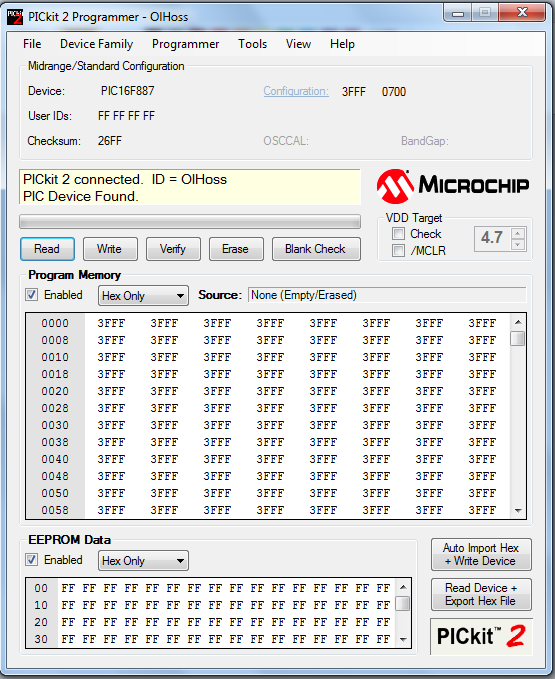
\includegraphics[scale=.5]{phu-luc/image/pickit-21}
\end{center}
\caption{Giao diện của phần mềm PICKit 2 Programmer}
\label{Fig:PICKIT-2}
\end{figure}
\begin{itemize}
\item Thẻ \verb|Tab|:
\begin{list}{--}{}
\item \verb|Import Hex|: Tải một file Hex vào bộ nhớ tạm.
\item \verb|Export Hex|: Xuất ra một file Hex có trong bộ nhớ tạm.
\end{list}
\item Thẻ \verb|Programmer|:
\begin{list}{--}{}
\item \verb|Read Device|: đọc nội dung chip như \verb|Program memory|, \verb|EEPROM data| đưa vào bộ nhớ tạm.
\item \verb|Write  Device|: nạp nội dung như \verb|Program  memory|, \verb|EEPROM data| đưa vào bộ nhớ tạm vào chip.
\item \verb|Verify|: so sánh nội dung của chip với nội dung trong bộ nhớ tạm.
\item \verb|Erase|: Xóa toàn bộ nội dung trong chip.
\end{list}
\item Thẻ \verb|Tools|:
\begin{list}{--}{}
\item \verb|Enable Code Protect|: khóa chương trình, chống sao chép.
\item \verb|Enable Data Protect|: khóa bộ nhớ \verb|EEPROM data| chống sao chép.
\item \verb|Fast programming|: nếu chọn chức năng này thì PICKit 2 sẽ nạp nhanh hơn, bình thường (chưa chọn) thì sẽ nạp chậm và độ tin cậy cao hơn.
\item \verb|Check Communication|: Kiểm tra giao tiếp giữa PC với PICkit 2 và ICSP giúp dò tìm chip.
\end{list}
\end{itemize}
\tocless \section{Nạp chương trình cho PIC}
Thực hiện theo các bước:
\begin{list}{--}{}
\item \textit{Bước 1}: Vào thẻ \verb|Tools| chọn \verb|Check Communication| để kiểm tra và dò tìm PIC tự động: 
\begin{list}{+}{}
\item Nếu nhận được PIC thì dòng \verb|Device| sẽ hiện tên PIC (như trong \textit{hình \ref{Fig:PICKIT-2}} là PIC16F887).
\item Không nhận được chip thì kiểm tra lại kết nối USB, cách gắn PIC lên Adapter có đúng chiều hay chưa.
\end{list}
\item \textit{Bước 2}: Vào thẻ \verb|File| chọn \verb|Import Hex| rồi đi đến địa chỉ lưu file Hex cần nạp cho PIC. Rồi Click chọn \verb|Open| để mở file Hex lưu vào bộ nhớ tạm.
\item \textit{Bước 3}: Click chọn \verb|Write| để ghi nội dung từ bộ nhớ tạm vào PIC.
\end{list}
Nếu nạp thành công sẽ có giao diện như \textit{hình \ref{Fig:PICKIT-2-1}}, các trường hợp khác là chưa nạp thành công (không xuất hiện màu xanh lá như hình \ref{Fig:PICKIT-2-1} mà xuất hiện màu đỏ).
\begin{figure}[!h]
\begin{center}
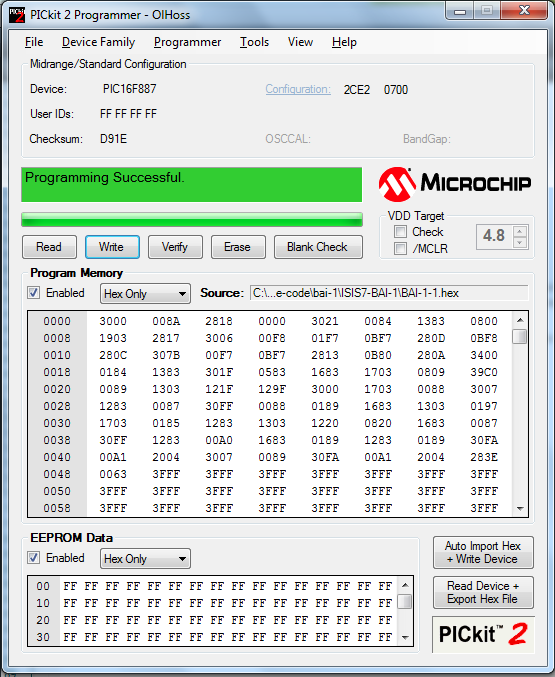
\includegraphics[scale=.5]{phu-luc/image/pickit-22}
\end{center}
\caption{Giao diện khi nạp thành công chương trình cho PIC}
\label{Fig:PICKIT-2-1}
\end{figure}

Ngoài ra cũng cần lưu ý ô điện áp \verb|VDD Target| thông thường từ $4.7V - 5V$.
\chapter{Thư viện DEF\_887.H}\label{def:887}
%\addcontentsline{toc}{chapter}{Thư viện DEF\_887.H}
Nội dung file \verb|DEF_887.H| (tên định danh của các PORT, các chân và thanh ghi).
\lstinputlisting[language=C]{DEF_887.H}
\chapter{Thư viện LCD\_LIB\_4BIT.C}\label{def:lcd}
Nội dung file \verb|LCD_LIB_4BIT.C|
\lstinputlisting[language=C]{LCD_LIB_4BIT.C}
\chapter{Hiển thị với LED 7 đoạn}
\label{app:led-7-doan}
\tocless \section{Giới thiệu}
LED 7 đoạn có 2 loại là Anode chung hoặc Kathode chung, ở dạng một LED 7 đoạn hoặc nhiều LED 7 đoạn ghép lại với nhau.

Gồm 7 LED đơn mắc với nhau theo thứ tự có thể hiển thị được các số từ $0 - 7$ (ngoài ra có thể có thêm dấu \verb|"."| để phân cách nhiều LED 7 đoạn với nhau), ta gọi các LED đơn này là $a$, $c$, $c$, $d$, $e$, $f$, $g$ (có thể có thêm $dp$).
\begin{figure}[!h]
\begin{center}
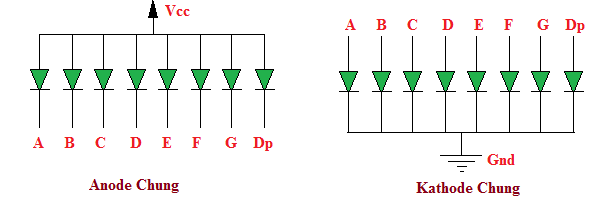
\includegraphics[scale=.6]{phu-luc/image/led-7-seg}
\end{center}
\caption{Sơ đồ chân của LED 7 đoạn}
\end{figure}
\begin{figure}[!h]
\begin{center}
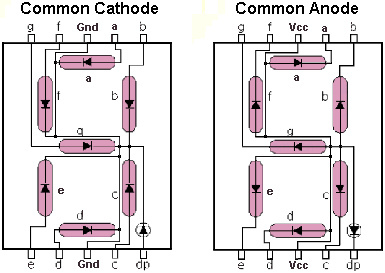
\includegraphics[scale=.4]{phu-luc/image/led-7-seg-anode-kathode}
\end{center}
\caption{Sơ đồ chân của LED 7 đoạn Anode hoặc Kathode chung ngoài thực tế}
\end{figure}
\tocless \subsection{LED 7 đoạn có Anode chung}
\begin{itemize}
\item Để hiển thị thanh LED nào, ta chỉ cần nối xuống chân $K$ của thanh LED đó xuống mass.
\item Sử dụng điện trở để hạn dòng cho LED.
\item Mã LED 7 đoạn Anode chung:
\begin{table}[!h]
\begin{center}
\begin{tabular}{|c|c|c|c|c|c|c|c|c|c|c|c|}\hline
\multirow{3}{.5cm}{\centering{Số}} & \multicolumn{8}{|c|}{Mã nhị phân} & \multicolumn{2}{|c|}{Mã HEX}\\ \cline{2-9}
& 7 & 6 & 5 & 4 & 3 & 2 & 1 & 0 & \multicolumn{2}{c|}{}\\ \cline{2-11}
& dp & g & f & e & d & c & b & a & dp & \\ \hline
0 & dp & 1 & 0 & 0 & 0 & 0 & 0 & 0 &  40 & C0\\ \hline
1 & dp & 1 & 1 & 1 & 1 & 0 & 0 & 1 &  79 & F9\\ \hline
2 & dp & 0 & 1 & 0 & 0 & 1 & 0 & 0 &  24 & A4\\ \hline
3 & dp & 0 & 1 & 1 & 0 & 0 & 0 & 0 &  30 & B0\\ \hline
4 & dp & 0 & 0 & 1 & 1 & 0 & 0 & 1 &  19 & 99\\ \hline
5 & dp & 0 & 0 & 1 & 0 & 0 & 1 & 0 &  12 & 92\\ \hline
6 & dp & 0 & 0 & 0 & 0 & 0 & 1 & 0 &  02 & 82\\ \hline
7 & dp & 1 & 1 & 1 & 1 & 0 & 0 & 0 &  78 & F8\\ \hline
8 & dp & 0 & 0 & 0 & 0 & 0 & 0 & 0 &  00 & 80\\ \hline
9 & dp & 0 & 0 & 1 & 0 & 0 & 0 & 0 &  10 & 90\\ \hline
A & dp & 0 & 0 & 0 & 1 & 0 & 0 & 0 &  08 & 88\\ \hline
B & dp & 0 & 0 & 0 & 0 & 0 & 1 & 1 &  03 & 83\\ \hline
C & dp & 1 & 0 & 0 & 0 & 1 & 1 & 0 &  46 & C6\\ \hline
D & dp & 0 & 1 & 0 & 0 & 0 & 0 & 1 &  21 & A1\\ \hline
E & dp & 0 & 0 & 0 & 0 & 1 & 1 & 0 &  06 & 86\\ \hline
F & dp & 0 & 0 & 0 & 1 & 1 & 1 & 0 &  0E & 8E\\ \hline
\end{tabular}
\end{center}
\caption{Mã LED 7 đoạn Anode chung}\label{Fig:led-7-seg-anode}
\end{table}
\end{itemize}
\tocless \subsection{LED 7 đoạn có Kathode chung}
\begin{itemize}
\item Để hiển thị thanh LED nào, ta chỉ cần nối xuống chân $A$ của thanh LED đó lên nguồn.
\item Sử dụng điện trở để hạn dòng cho LED.
\item Mã LED 7 đoạn Kathode chung:
\begin{table}[!h]
\begin{center}
\begin{longtable}{|c|c|c|c|c|c|c|c|c|c|c|c|}\hline
\multirow{3}{.5cm}{\centering{Số}} & \multicolumn{8}{|c|}{Mã nhị phân} & \multicolumn{2}{|c|}{Mã HEX}\\ \cline{2-9}
& 7 & 6 & 5 & 4 & 3 & 2 & 1 & 0 & \multicolumn{2}{c|}{}\\ \cline{2-11}
& dp & g & f & e & d & c & b & a & dp & \\ \hline
0 & dp & 0 & 1 & 1 & 1 & 1 & 1 & 1 &  BF & 3F\\ \hline
1 & dp & 0 & 0 & 0 & 0 & 1 & 1 & 0 &  86 & 06\\ \hline
2 & dp & 1 & 0 & 1 & 1 & 0 & 1 & 1 &  DB & 5B\\ \hline
3 & dp & 1 & 0 & 0 & 1 & 1 & 1 & 1 &  CF & 4F\\ \hline
4 & dp & 1 & 1 & 0 & 0 & 1 & 1 & 0 &  E6 & 66\\ \hline
5 & dp & 1 & 1 & 0 & 1 & 1 & 0 & 1 &  ED & 6D\\ \hline
6 & dp & 1 & 1 & 1 & 1 & 1 & 0 & 1 &  FD & 7D\\ \hline
7 & dp & 0 & 0 & 0 & 0 & 1 & 1 & 1 &  87 & 07\\ \hline
8 & dp & 1 & 1 & 1 & 1 & 1 & 1 & 1 &  FF & 7F\\ \hline
9 & dp & 1 & 1 & 0 & 1 & 1 & 1 & 1 &  EF & 6F\\ \hline
A & dp & 1 & 1 & 1 & 0 & 1 & 1 & 1 &  F7 & 77\\ \hline
B & dp & 1 & 1 & 1 & 1 & 1 & 0 & 0 &  FC & 7C\\ \hline
C & dp & 0 & 1 & 1 & 1 & 0 & 0 & 1 &  B9 & 39\\ \hline
D & dp & 1 & 0 & 1 & 1 & 1 & 1 & 0 &  DE & 5E\\ \hline
E & dp & 1 & 1 & 1 & 1 & 0 & 0 & 1 &  F9 & 79\\ \hline
F & dp & 1 & 1 & 1 & 0 & 0 & 0 & 1 &  F1 & 71\\ \hline
\end{longtable}
\end{center}
\caption{Mã LED 7 đoạn Kathode chung}\label{Fig:led-7-seg-kathode}
\end{table}
\end{itemize}
\tocless \subsection{IC ghi dịch 74HC595}
\begin{figure}[!h]
\begin{center}
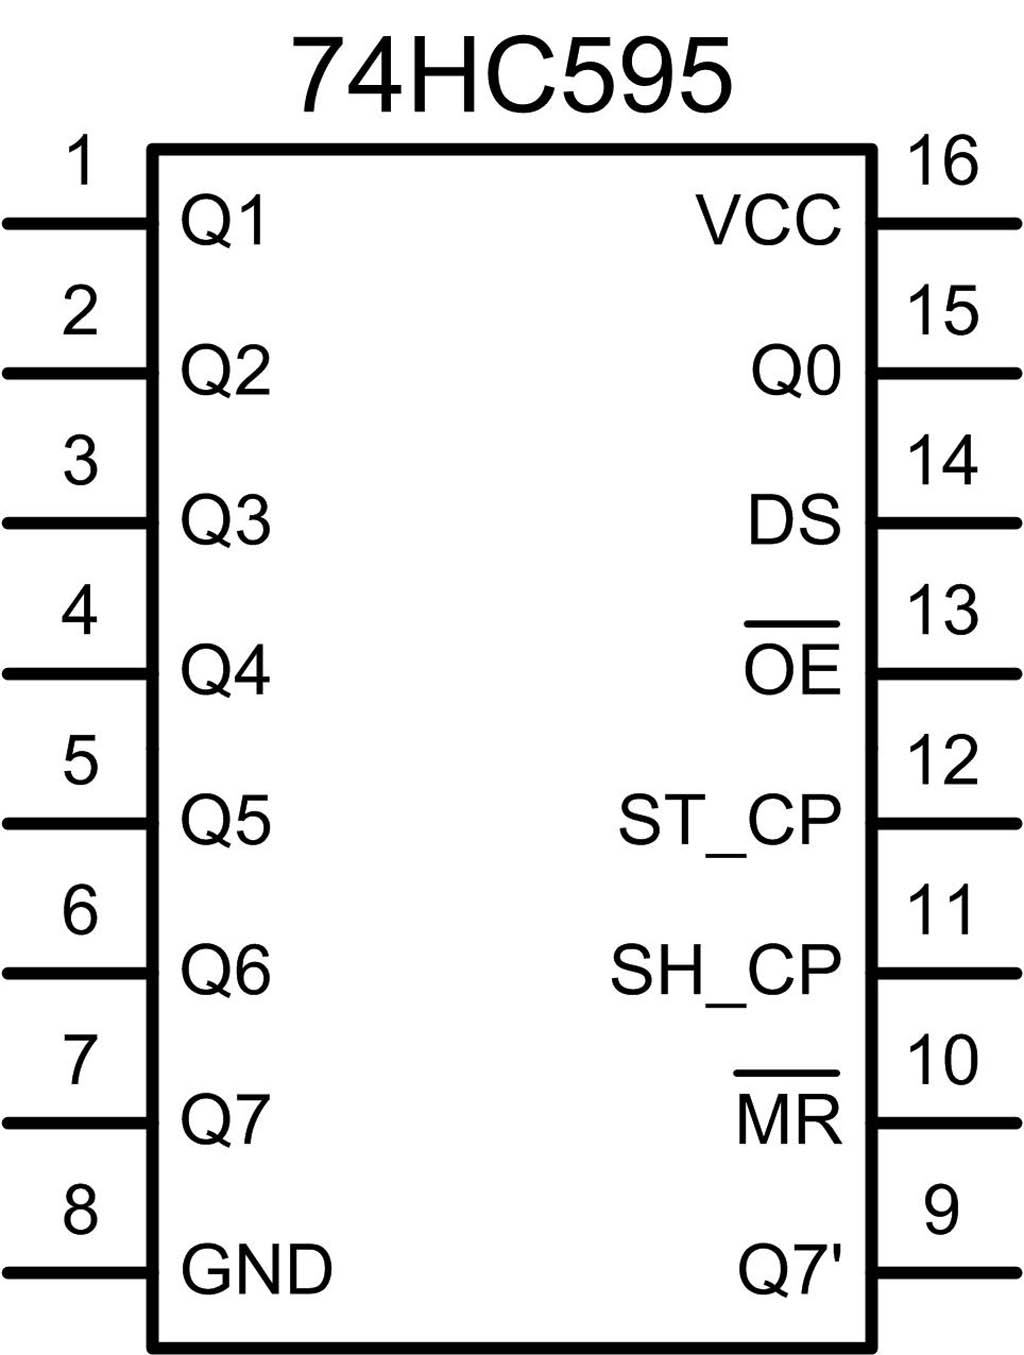
\includegraphics[scale=1.5]{phu-luc/image/74HC595}
\end{center}
\caption{Sơ đồ chân của IC ghi dịch 74HC595}\label{Fig:ngly-74hc595}
\end{figure}
Nguyên lý hoạt động của IC 74HC595:hình \ref{Fig:ngly-74hc595}
\begin{itemize}
\item Mô tả chức năng các chân:
\begin{itemize}
\item Input: chân $DS$: đầu vào dữ liệu nối tiếp. Tại mỗi thời điểm chỉ đưa vào 1 bit.
\item Output: từ chân $Q0 - Q7$. Xuất dữ liệu khi chân $\overline{OE}$ tích cực ở mức thấp và có một xung tích cực ở sườn âm tại chân chốt $ST\_CP$.
\item Output -- Enable: chân $\overline{OE}$: chân cho phép tích cực ở mức thấp. Khi nó ở mức cao thì không đầu ra nào được cho phép.
\item SQH: chân $Q7^\prime$: chân dữ liệu nối tiếp. Dùng để nối tiếp với IC 75HC595 khác, dữ liệu sẽ truyền cho IC tiếp theo khi nó đã nhận đủ được 8 bit.
\item Shift clock: chân $SH\_CP$: khi có một xung clock tích cực ở sườn dương thì 1 bit được dịch vào IC.
\item Latch clock: chân $ST\_CP$: xung chốt dữ liệu. Khi có một xung clock tích cực ở sườn dương thì cho phép xuất dữ liệu.
\item Chiều dịch bit: từ $Q0 \rightarrow Q7$.
\item Reset: chân $\overline{MR}$: chân này ở mức thấp thì dữ liệu sẽ bị xóa.
\end{itemize}
\item Nguyên lý hoạt động:
\begin{itemize}
\item Khi 1 bit được đưa vào chân $DS$, muốn đẩy bit này vào thanh ghi thì phải kích một xung vào chân $SH\_CP$ (xung sườn dương từ 0 lên 1). Làm như vậy, cho đến khi thanh ghi đủ 8 bit.
\item Dữ liệu 8 bit trong thanh ghi vẫn chưa thể xuất ra được, cần tạo một xung lên chân $ST\_CP$ (xung sườn dương từ 0 lên 1).
\item Khi dữ liệu quá 8 bit thì số bit còn dư sẽ đươc đưa đến chân $Q7^\prime$. Kết nối chân $Q7^\prime$ với chân $DS$ của IC tiếp theo để mở rộng chân.
\end{itemize}
\end{itemize}
\tocless \section{Phương pháp điều khiển}
Ta xét 2 phương pháp điều khiển: trực tiếp qua các chân \verb|I/O| và gián tiếp qua IC ghi dịch.
\begin{itemize}
\item Phương pháp điều khiển trực tiếp qua các chân \verb|I/O|:
\begin{itemize}
\item Ưu điểm: đơn giản.
\item Nhược điểm: tốn nhiều chân của vi điều khiển, không thể điều khiển số lượng lớn các LED 7 đoạn.
\end{itemize}
\item Phương pháp điều khiển gián tiếp qua IC ghi dịch:
\begin{itemize}
\item Ưu điểm: Dùng ít chân để điều khiển LED 7 đoạn (với IC 74HC595 chỉ dùng 3 chân của vi điều khiển có thể điều khiển được nhiều LED qua các IC ghi dịch này và có thể kết nối nhiều IC ghi dịch lại với nhau).
\item Khuyết điểm: phức tạp hơn phương pháp điều khển trực tiếp.
\end{itemize}
\end{itemize}
Khi sử dụng nhiều LED 7 đoạn được ghép chung với nhau, ta nên sử dụng phương pháp quét LED (bật tắt các LED một cách liên tục).
\tocless \section{Yêu cầu}
\paragraph{Yêu cầu 1}Sử dụng LED 7 đoạn đếm các số từ $0 - 9$ và từ $A-F$ bằng 2 phương pháp (điều khiển trực tiếp và điều khiển thông qua IC 74HC595).
\tocless \subsection{Phương pháp điều khiển trực tiếp}
\paragraph{Hướng giải quyết} Ta xuất giá trị của mã code ứng với loại LED 7 đoạn có Anode chung hay Kathode chung cho trong \textit{bảng \ref{Fig:led-7-seg-anode}} hoặc \textit{bảng \ref{Fig:led-7-seg-kathode}}.
\paragraph{Sơ đồ mạch}{~\\}
\begin{figure}[!h]
\begin{center}
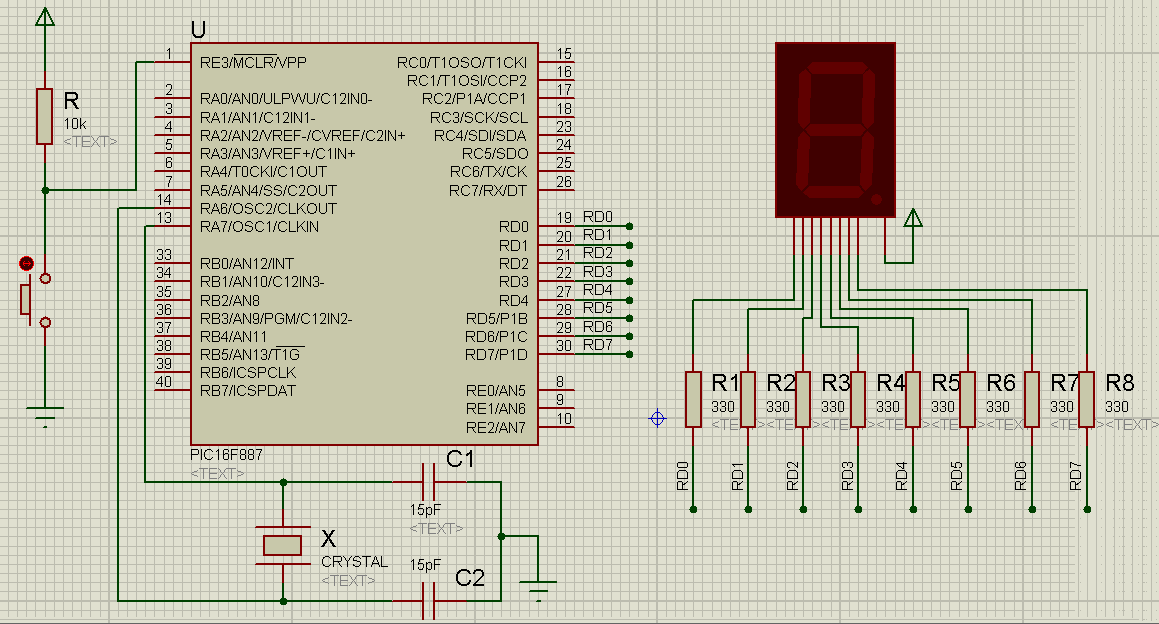
\includegraphics[scale=.5]{phu-luc/image/bai-2-phu-luc-led-7-seg}
\end{center}
\caption{Sơ đồ mạch điều khiển một LED 7 đoạn}
\end{figure}
\paragraph{Chương trình}{~\\}
\lstinputlisting[language=C]{BAI-2-PHU-LUC-LED-7-SEG-V1.C}
\newpage
\tocless \subsection{Phương pháp điều khiển thông qua IC ghi dịch 74HC595}
\paragraph{Sơ đồ mạch}{~\\}
\begin{figure}[!h]
\begin{center}
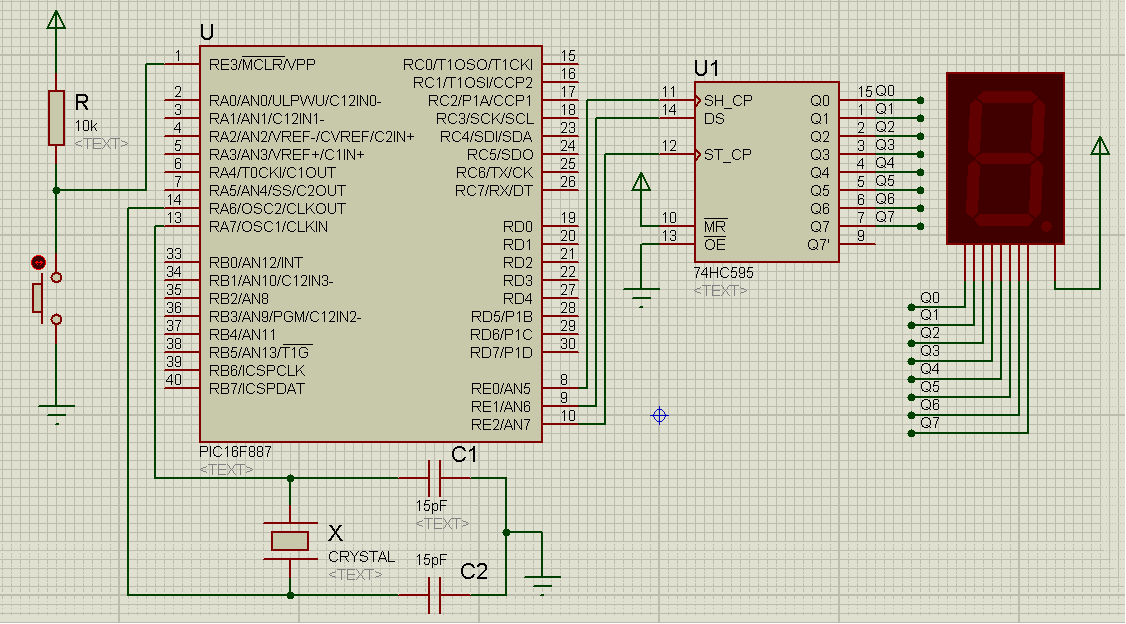
\includegraphics[scale=.5]{phu-luc/image/bai-2-phu-luc-led-7-seg-74hc595}
\end{center}
\caption{Sơ đồ mạch điều khiển một LED 7 đoạn qua IC 74HC595}
\end{figure}
\paragraph{Chương trình}{~\\}
\lstinputlisting[language=C]{BAI-2-PHU-LUC-LED-7-SEG-V2.C}
\paragraph{Yêu cầu 2}Sử dụng 4 LED 7 đoạn hiển thị các số từ $0 - 9999$ bằng 2 phương pháp (điều khiển trực tiếp bằng các chân và điều khiển thông qua IC 74HC595).
\tocless \subsection{Phương pháp quét LED -- Điều khiển trực tiếp qua các chân của vi điều khiển}
\paragraph{Sơ đồ mạch}{~\\}
\begin{figure}[!h]
\begin{center}
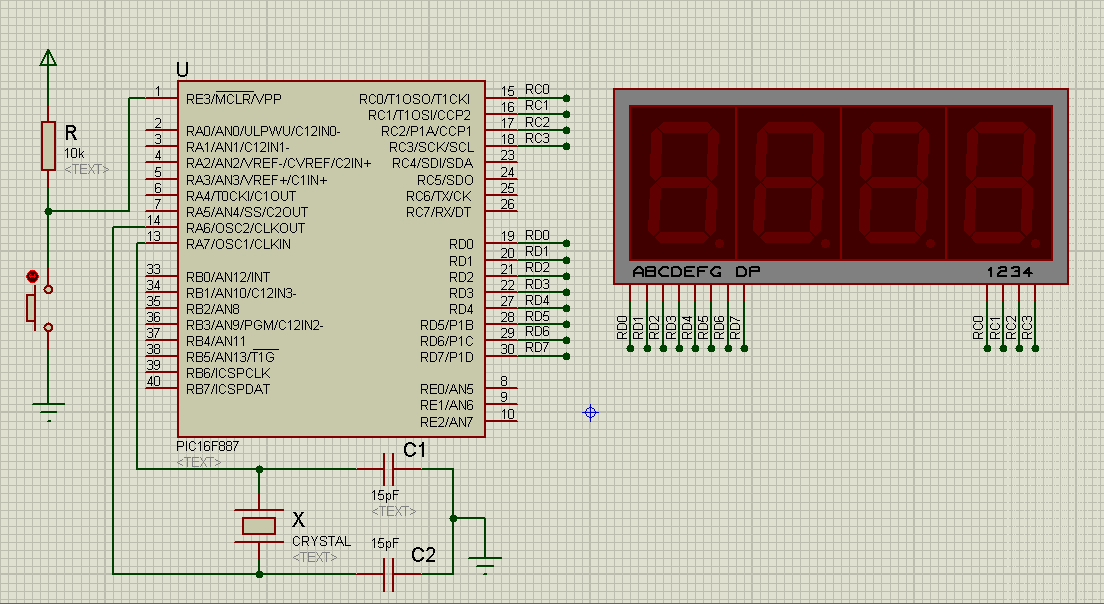
\includegraphics[scale=.5]{phu-luc/image/bai-2-phu-luc-4-led-7-seg}
\end{center}
\caption{Sơ đồ mạch điều khiển 4 LED 7 đoạn}
\end{figure}
\paragraph{Hướng giải quyết}
\begin{itemize}
\item Thường các LED loại này các thanh $a,b,c,d,e,f,g$ (có thể có $dp$) là chung với nhau, nó chỉ phân biệt nhau bằng số tự của LED 7 đoạn (mỗi LED 7 đoạn sẽ có một chân điều khiển).
\item Do đó, để hiển thị với nhiều LED 7 đoạn, ta dùng phương pháp quét LED: lặp lại quá trình bậc tắt các LED, khi đó sẽ đánh lừa được thị giác con người (do mắt người chỉ nhìn thấy được 24 điểm ảnh trên $1s$).
\item Với \textit{yêu cầu 2}, ta cần tách ra các chữ số riêng lẻ từ số ban đầu, rồi cho mỗi LED 7 đoạn hiển thị một số.
\end{itemize}
\paragraph{Chương trình}{~\\}
\lstinputlisting[language=C]{BAI-2-PHU-LUC-4-LED-7-SEG-V1.C}
\tocless \subsection{Phương pháp quét LED -- Điều khiển thông qua IC 74HC595}
\paragraph{Sơ đồ mạch}{~\\}
\begin{figure}[!h]
\begin{center}
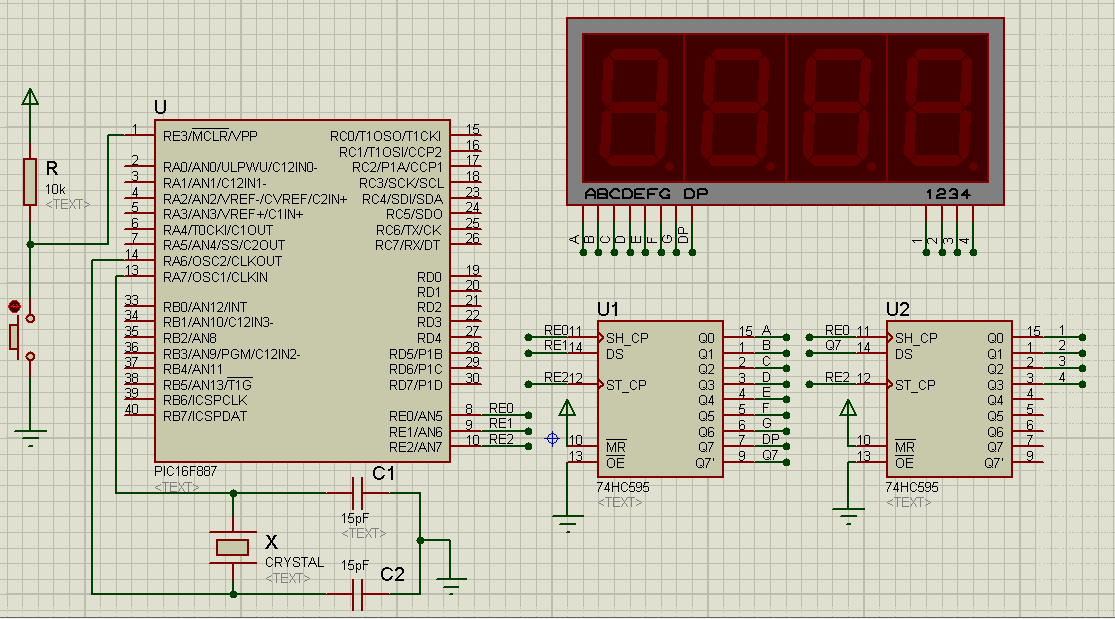
\includegraphics[scale=.5]{phu-luc/image/bai-2-phu-luc-4-led-7-seg-74hc595}
\end{center}
\caption{Sơ đồ mạch điều khiển 4 LED 7 đoạn qua IC 74HC595}
\end{figure}
\paragraph{Hướng giải quyết}
\begin{itemize}
\item Để tiết kiệm số chân điều khiển của vi điều khiển, ta dùng 2 IC 75HC595 để điều khiển 4 LED 7 đoạn.
\item Hoạt động theo nguyên tắc ngăn xếp: đưa vào sau sẽ lấy ra trước.
\item IC đầu tiên khi nhận đủ 8 bit, nếu tiếp tục gửi bit thì nó sẽ chuyển số bit dư sang chân $Q7^\prime$ để chuyển sang IC thứ 2.
\end{itemize}
\paragraph{Chương trình}{~\\}
\lstinputlisting[language=C]{BAI-2-PHU-LUC-4-LED-7-SEG-V2.C}

%\chapter{Đọc tín hiệu từ nút nhấn}\label{Code:Button 3-2}
%Nội dung file \verb|INPUT_BUTTON.C| (Một cách làm khác của \textit{bài tập 3.2} trang \pageref{Ex:3-2}).
%\lstinputlisting[language=C]{INPUT_BUTTON.C}
\chapter{Thư viện RTC DS3231} \label{def:DS3231}
Thư viện gồm 2 file \verb|DS3231.H| và \verb|DS3231.C| được viết bời tác giả \verb|sshahryiar| trên diễn đàn \verb|https://www.ccsinfo.com|\footnote{https://www.ccsinfo.com/forum/viewtopic.php?t=50256}
\section*{Nội dung file DS3231.H}
\lstinputlisting[language=C]{DS3231.H}
\section*{Nội dung file DS3231.C}
\lstinputlisting[language=C]{DS3231.C}
\begin{comment}
\chapter{Mô phỏng cảm biến nhiệt TC74 với Protues}\label{def:TC74}
Trong quá trình tìm hiểu, em thấy có nhiều bạn gặp vấn đề khi mô phỏng cảm biến nhiệt độ TC74 với phần mềm protues. Em kiểm thử, và phát hiện được là cảm biến nhiệt \verb|TC74| trong phần mềm mô phỏng \verb|Protues 7.8| nó tương thích với địa chỉ \verb|I2C| là \verb|0x9A| (đa phần các bạn làm trên địa chỉ \verb|0x90| nên khi mô phỏng thì ra giá trị nhiệt độ không mong muốn).

Về sơ đồ mạch và cách giải thích chương trình tương tự \textit{bài tập 6.1 trang \pageref{Ex:6-1}}.
\paragraph{Chương trình sau mô phỏng được với phần mềm Protues 7.8}{~\\}
\lstinputlisting[language=C]{BAI-6-1V2.C}
\end{comment}
\begin{comment}
\chapter{Điều khiển tốc độ động cơ với Transistor}
\paragraph{Sơ đồ mạch}{~\\}
\begin{figure}[!h]
\begin{center}
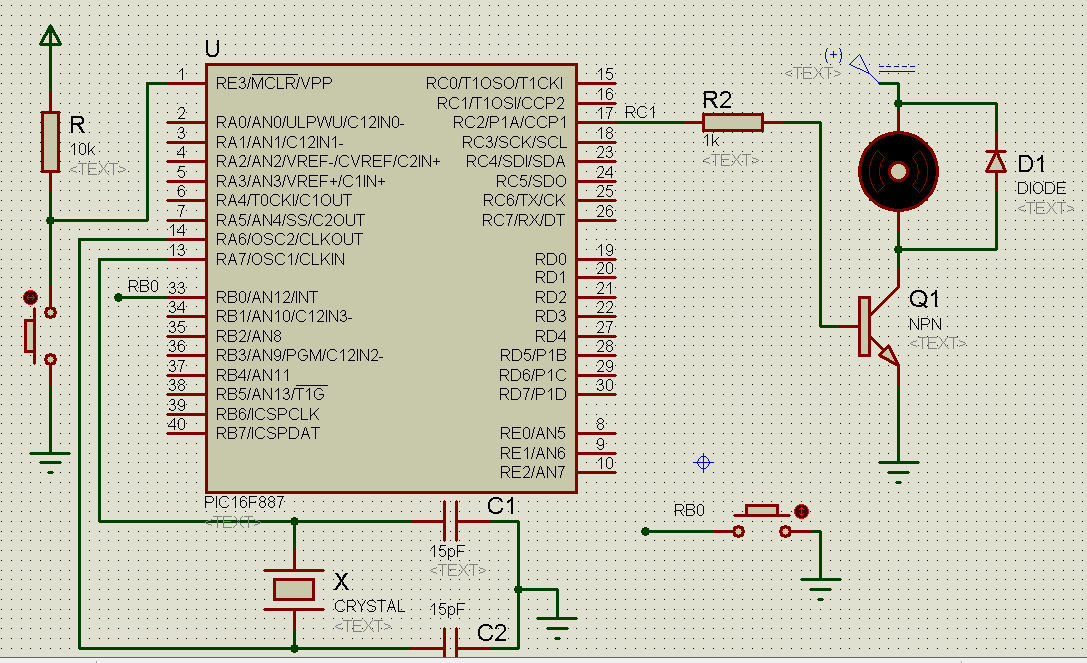
\includegraphics[scale=.5]{bai-8/image/BAI-8-2-2}
\end{center}
\caption{Điều khiển tốc độ động cơ bằng qua kích Transistor}
\end{figure}\\

Nội dung của chương trình: 
\lstinputlisting[language=C]{BAI-8-2-1.C}
\end{comment}
\chapter{Các khai báo sau \#FUSES}
%Trong phần đầu chương trình chúng ta có sử dụng các từ viết tắt khái báo sau \verb|#FUSES|, các từ này có ý nghĩa như sau:
\begin{table}[!h]
\vspace{-2cm}
\begin{center}
\begin{longtable}{|c|c|c|c|}\hline
\textit{STT} & \textit{Từ viết tắt} & \multicolumn{2}{|c|}{\textit{Ý nghĩa}} \\ \hline
\multicolumn{4}{|c|}{\textit{WATCH DOG TIMER}}\\ \hline
1 & \verb|NOWDT| & \multicolumn{2}{|l|}{Không sử dụng bộ Watch Dog Timer} \\ \hline
2 & \verb|WDT| & \multicolumn{2}{|l|}{Sử dụng bộ Watch Dog Timer} \\ \hline
\multicolumn{4}{|c|}{\textit{HIGH SPEED OSC}}\\ \hline
3 & \verb|LP| & \multicolumn{2}{|l|}{Sử dụng nguồn dao động tần số thấp $f<200kHz$} \\ \hline
4 & \verb|XT| & \multicolumn{2}{|l|}{Dao động thạch anh $f<4MHz$ với PCM/PCH} \\ \cline{3-4}
 &  & \multicolumn{2}{|l|}{Dao động thạch anh $f=3MHz-10MHz$ với PCD} \\ \hline
5 & \verb|RC| & \multicolumn{2}{|l|}{Dao động RC với CLKOUT} \\ \hline
6 & \verb|HS| & \multicolumn{2}{|l|}{Dao động tần số cao} \\ \cline{3-4}
 &  & \multicolumn{2}{|l|}{$f>4MHz$ với PCM/PCH hoặc $f>10MHz$ với PCD} \\ \hline
 \multicolumn{4}{|c|}{\textit{POWER UP TIMER}}\\ \hline
7 & \verb|NOPUT| & \multicolumn{2}{|l|}{Không sử dụng Power Up Timer} \\ \hline
8 & \verb|PUT| & \multicolumn{2}{|l|}{Sử dụng Power Up Timer} \\ \hline
\multicolumn{4}{|c|}{\textit{BROWN OUT}}\\ \hline
9 & \verb|NOBROWNOUT| & \multicolumn{2}{|l|}{Không reset chip khi BrownOut} \\ \hline
10 & \verb|BROWNOUT| & \multicolumn{2}{|l|}{Reset chip khi BrownOut} \\ \hline
\multicolumn{4}{|c|}{\textit{LOW VOLTAGE PROGRAM}}\\ \hline
11 & \verb|NOLVP| & \multicolumn{2}{|l|}{Không lập trình điện áp thấp, B3 (PIC16); B5 (PIC18) là I/O} \\ \hline
12 & \verb|LVP| & \multicolumn{2}{|l|}{Lập trình điện áp thấp trên B3 (PIC16); B5 (PIC18)} \\ \hline
\multicolumn{4}{|c|}{\textit{CODE PROTECED EEPROM}}\\ \hline
13 & \verb|NOCPD| & \multicolumn{2}{|l|}{Không bảo vệ dữ liệu EEPROM} \\ \hline
14 & \verb|CPD| & \multicolumn{2}{|l|}{Bảo vệ dữ liệu EEPROM} \\ \hline
\multicolumn{4}{|c|}{\textit{PROGRAM WRITE PROTECED}}\\ \hline
15 & \verb|WRT| & \multicolumn{2}{|l|}{Bộ nhớ chương trình viết được bảo vệ} \\ \hline
16 & \verb|WRT_50%| & \multicolumn{2}{|l|}{Nửa phần dưới của bộ nhớ chương trình viết được bảo vệ} \\ \hline
17 & \verb|WRT_5%| & \multicolumn{2}{|l|}{Bộ nhớ chương trình viết ít hơn 255 byte thì được bảo vệ} \\ \hline
18 & \verb|NOWRT| & \multicolumn{2}{|l|}{Bộ nhớ chương trình viết không được bảo vệ} \\ \hline
\multicolumn{4}{|c|}{\textit{DEBUG FOR ICD}}\\ \hline
19 & \verb|NODEBUG| & \multicolumn{2}{|l|}{Không sử dụng chế độ Debug với ICD} \\ \hline
20 & \verb|DEBUG| & \multicolumn{2}{|l|}{Sử dụng chế độ Debug với ICD} \\ \hline
\multicolumn{4}{|c|}{\textit{CODE PROTECED FROM READING}}\\ \hline
21 & \verb|NOPROTECT| & \multicolumn{2}{|l|}{Cho phép đọc lại code} \\ \hline
22 & \verb|PROTECT| & \multicolumn{2}{|l|}{Không cho phép đọc lại code} \\ \hline
\end{longtable}
\end{center}
\vspace{-.4cm}
\caption{Ý nghĩa của các khai báo trong \#FUSES}
\end{table}
\end{document}
